%%%%%%%%%%%%%%%%%%%%%%%%%%%%%%%%%%%%%%
% yale_thesis.tex
% Alexander Cerjan
% 2014/04/07
%
% A bare, sample template for a Yale PhD thesis using yalephd.cls
%%%%%%%%%%%%%%%%%%%%%%%%%%%%%%%%%%%%%%

\documentclass[letterpaper,11pt]{yalephd}
% remove draft option for final printing.
% font size must be between 10pt-12pt.

\usepackage{geometry} % you need this for yalephd.cls to work.
\usepackage{graphicx} % you probably want the rest of these.
\usepackage{dcolumn}
\usepackage{bm}
\usepackage{amsmath}
\usepackage{amsfonts}
\usepackage{amssymb}
\usepackage{appendix}
\usepackage{comment}
\usepackage{cite}
\usepackage{notoccite}
\usepackage{afterpage}
\usepackage{bibentry}
\usepackage{longtable}
\usepackage{supertabular}
\usepackage{lipsum}
\usepackage{cleveref}
\usepackage{indentfirst}
\usepackage{notoccite}

\nobibliography*

\bibliographystyle{abbrvunsrt}

\newcommand\textbox[1]{%
  \parbox{.5\textwidth}{#1}%
}

\begin{document}

% Need to define title before the abstract.
\title{Title goes here}
\author{John Gockley}
\advisor{James Noonan}
\date{May, 2017} % usually not \today.

% All the stuff at the front of your thesis.
\frontmatter

\begin{abstract}
\textbf{Part One:}\\
A 4:1 male to female sex bias has consistently been observed in autism spectrum disorder (ASD). Epidemiological and genetic studies suggest a female protective effect (FPE) may account for part of this bias; however, the mechanism of such protection is unknown. Quantitative assessment of ASD symptoms using the Social Responsiveness Scale (SRS) shows a bimodal distribution unique to females in multiplex families. This leads to the hypothesis that a single, common genetic locus on chromosome X might mediate the FPE and produce the ASD sex bias. Such a locus would represent a major therapeutic target and is likely to have been missed by conventional GWAS analysis. To explore this possibility an association study in affected versus unaffected females was preformed, considering three tiers of SNPs: 1) regions of chromosome X that escape X-inactivation; 2) all of chromosome X; and 3) genome-wide. No evidence of a SNP meeting the criteria for a single FPE locus was observed, despite the analysis being well powered to detect this effect. The results do not support the hypothesis that the FPE is mediated by a single genetic locus, however this does not exclude the possibility of multiple genetic loci playing a role in the FPE.\\ 
\textbf{Part Two:}\\
Noonan Abstract here 546 word limit

\end{abstract}

\maketitle
\makecopyright{2017} % change as needed.

\tableofcontents

\listoffigures % remove this if you have no figures.

\listoftables % remove this if you have no tables.

\chapter{Acknowledgements} % this needs to be before \mainmatter.
	People, GPSCY, Hockey, etc..

\chapter{Forward}
	Two Part Thesis Etc. 

\chapter{Communications from this PhD Candidacy}
\bigskip
\bibentry{Willsey:2013aa}\bigskip
 
\bibentry{Dong:2014aa}\bigskip

\bibentry{Gockley:2015aa}\bigskip

\bibentry{Emera:2016aa}

% Starts proper arabic numbering of pages and chapters.
\mainmatter

\chapter{Autism Spectrum Disorders}
	\section{Background}
    	\setlength{\parindent}{10ex}\par
        Autism Spectrum Disorders ASDs is characterized by deficits in language development, impairment of social reciprocity, and repetitive behaviors or restricted interests. ASDs are prevalent in society affecting one of every 68 children in the United States \cite{Developmental-Disabilities-Monitoring-Network-Surveillance-Year-2010-Principal-Investigators:2014aa}.  While global ASD prevalence has risen sharply since the 1960’s and 70’s, studies indicate this increase is most likely due to greater testing sensitivity, closer monitoring of child mental development, and increased cultural awareness of mental health as an entirety; not as a result of increased incidence \cite{Fombonne:2009aa}. Interestingly ASDs are not only highly heritable \cite{Ozonoff:2011aa} but also exhibit a surprisingly strong sex bias, presenting a 4.2:1 to 4.5:1 male to female sex bias \cite{Developmental-Disabilities-Monitoring-Network-Surveillance-Year-2010-Principal-Investigators:2014aa,Fombonne:2009aa}.\par
        
        Through studying ASD prevalence between dizygotic twins, ASD has been estimated to be up to 90\% heritable \cite{Bailey:1995aa,Muhle:2004aa,Rosenberg:2009aa}. Occurrence rates amongst siblings, with an affected older sibling, are 18.9\% higher than the general population. ASD sex bias is highly divergent in contributing to overall re-occurrence with a rate of 26.2\% male siblings and only 9.1\% observed in female siblings. When multiplex families (families with more than 1 affected child) are considered re-occurrence rate in a third sibling are even higher, 32.2\% for males and 20.1\% for females, signaling an probable enrichment of heritable risk factors is present in the parents of multiplex families. \cite{Ozonoff:2011aa}.  Despite instances of syndromic X-linked disorders which preferentially affect females; Turner Syndrome \cite{Marco:2006aa}, Rett Syndrome \cite{Hagberg:1983aa}, and males: Klinefelter Syndrome \cite{Tartaglia:2008aa},  Fragile X Syndrome \cite{Aziz:2003aa,Reddy:2005aa}, these syndromic cases are excluded in the ~4:1 sex bias estimate. Such a dramatic sex bias represents an advantageous research target to elucidate the underlying genetic risk factors contributing towards autism. \par  

		The theory of a Female Protective Effect in ASD, where females have a higher phenotypic threshold towards ASD risk factors than males has gained support with recent data. The previously mentioned re-occurrence rates within families that contain an affected child, lead the initial insight into a potential FPE. The Carter Effect, first defined in Pyloric Stenosis \cite{CARTER:1961aa}, is the phenomena of a disorder having greater recurrence in proceeding offspring based on the sex of the index case. If females are protected from ASD one might expect that if the index case in a family is female, then the second child would have a greater probability of having autism compared to families where the index case was male. The basis for this is that in order to overcome an FPE the parents of an affected female would have greater ASD risk than those of a male proband.\par

	Observing the Carter Effect in ASDs is difficult in part due to the low prevalence of autism in females, and also as a result of an increased probability of families with an affected child tend to halt reproduction (stoppage). The more severe a given phenotype is in the child, the greater the rate of stoppage is \cite{Jones:1988aa}.  This further complicates the study of the Carter Effect in ASDs as females with a clinically diagnosed ASD tend to have a greater burden of risk and more severe phenotype \cite{Jacquemont:2014aa}. With a spectrum disorder, such as autism this would potentially affect families with a greater amount of risk factors.  Therefore families where the first child is an affected female would be pre-disposed towards halting reproduction reducing the power of a study to detect the Carter Effect.  Currently, two studies have observed the presence of the Carter Effect \cite{Sumi:2006aa,Ritvo:1989ab} while another two studies failed to see a significant correlation \cite{Goin-Kochel:2007aa,Ozonoff:2011aa}.\par

	To identify risk loci in ASD, the Simons Simplex Collection (SSC), a cohort of over 2,500 families with at least 2 children and only one proband, was utilized as this familial structure enriches for \textit{de novo} mutations which are expected to contribute greater risk towards an ASD phenotype relative to inherited risk factors. While enrichment of \textit{de novo} risk over heritable risk in simplex families is moderate, with an estimated heritability of 40\% instead of 60\% in simplex families illustrating the significant heritable risk in these cohorts \cite{Klei:2012aa}, the male to female sex bias raises as high as 7:1 \cite{Iossifov:2014aa}. While the change in ratio reduces the power to detect the Carter effect utilizing probands, there is a statistically significant enrichment of females in the unaffected sibling population relative to males. This could result from the SSC having removed multiplex families (families with more than one affected child), in which a subset of families could harbor large amounts of heritable risk capable of overcoming an FPE.\par

	While simplex cohorts have not been able to thoroughly investigate the Carter Effect in ASD, they provide a cohort enriched it higher effect \textit{de novo} mutations conferring ASD risk.  A study finding that a recurrent \textit{de novo} duplication of 7q13.23 Williams syndrome was statistically associated with autism \cite{Sanders:2011aa} sparked interest in whether recurrent \textit{de novo} CNVs in probands of simplex quartets could be leveraged to find regions which harbor autism risk.  Characterization of \textit{de novo} CNVs in the SSC found \textit{de novo} copy number variation to have a 4-fold increase in probands versus unaffected siblings, moreover these events were 1.6 times more frequent in female than male probands \cite{Sanders:2011aa}. One SSC study found that larger CNVs, which are more likely to be deleterious, were more likely to be maternally transmitted inferring that an FPE may allow mothers may carry more risk than fathers \cite{Jacquemont:2014aa}. However, exonic SNV transmission did not yield a significant differential paternal contribution\cite{ORoak:2012ab}. \par

	In addition to the increase in the number of events, CNVs in probands contained significantly more genes, increasing the likelihood of being disruptive and contributing towards an ASD phenotype. Gene enrichment within CNVs was further enriched in female probands, which averaged 15.5 genes per CNV, than male probands, which averaged 2 \cite{Levy:2011aa}.  Exome sequencing of the SSC supported CNV studies, reveling both an enrichment of likely gene disrupting mutations (LGD) such as; nonsense, frame shift and splice site as well as a slight enrichment in missense mutations \cite{Iossifov:2012aa,Sanders:2012ab,Neale:2012aa}. These events were also enriched in female probands compared to male probands. Additionally, affected females were shown to harbor an enrichment of \textit{de novo} indels \cite{Dong:2014aa}. This indicates that females are protected from ASD risk and require a greater burden of risk factors to exhibit an ASD phenotype than males.\par  

	SSC exome and indel studies were of particularly insightful due to the fact that recurrent LGD mutations in a single gene in probands versus siblings identified specific genes involved in autism. Of the 27 recurrent LGD, 353 single LGD, and 145 recurrent missense targets in probands versus siblings there is a 90\%, 40\%, and 35\% chance, respectively, of being implicated in ASD \cite{Iossifov:2014aa}.  Supporting the concept that females are protected from risk factors is the observation that when stratified by IQ males with a LGD \textit{de novo} mutation have a 5 point drop in non-verbal IQ, and males with a recurrent LGD \textit{de novo} have a 20 point drop in non-verbal IQ \cite{Iossifov:2014aa}.  Both statistically significant observations, point to these \textit{de novo} events carrying greater risk towards ASD diagnosis as intellectual disability (ID) tracks with increasing ASD severity and vise-versa\cite{OBrien:2004aa}. This supports claims that these \textit{de novo} events carry significant ASD risk, and that there enrichment in female probands is indicative of an FPE. 

	Although these \textit{de novo} studies have identified the first clear genes harboring ASD risk the vast majority of risk lies in common variation.  Current estimations put common inherited variation as contributing 49-55\% of all ASD liability while \textit{de novo} and rare inherited are only 3 and 4 percent respectively \cite{Gaugler:2014aa,Klei:2012aa}. The current challenge is how to identify the vast amount of common risk when sequencing studies are largely under-powered due to a relatively low effect size of any given common variant. While the amount of sequencing to gain the necessary power to examine common risk across the entire genome is staggering there are several approaches in which currently known risk can be used to mine existing data or to create new data sets which, in turn, can be leveraged to find novel risk factors or increase confidence in suspected risk factors.

	Specific enrichment in three broad processes of high confidence and the combined high confidence and probable set of genes harboring ASD risk identified in SSC simplex families has identified specific cellular pathways more likely to harbor as yet undiscovered ASD risk. Broadly, these enriched processes are Chromatin Regulation, Cell Proliferation/Motility \& Axonogensis, and Cell Communication/Synaptic Signaling \cite{De-Rubeis:2014aa,Pinto:2014aa}. Orthogonal methodology has utilized protein-protein interactions to identify genes with missense mutations more likely to contain ASD risk as a result of interacting with known high confident ASD risk genes. Taking these data sets a step forward, human brain spatio-temporal gene expression from fetal development through adolescence was used to find the genes most likely to be interacting with known ASD rick factors by seeding co-expression networks nine high confidence ASD risk genes. These networks were not only enriched in probable ASD genes, but this enrichment was specific to individual periods during fetal development. In addition genes within these networks at this midfetal time point were specifically expressed in layer 5/6 cortical glutamatergic neurons \cite{Willsey:2013aa}. 

	The enrichment of ASD risk in chromatin remodeling processes \cite{De-Rubeis:2014aa,Pinto:2014aa}  allows high confidence networks to be constructed empirically through chromatin immunoprecipitation (ChIP-Seq) and corresponding RNA-Seq data sets. One such study by Cotney et. al, focused on the highest confidence ASD risk factor to date, CHD8 a chromatin helicase. Gene promoters targets by CHD8 in hNSCs and human mid-fetal brain were highly enriched in probable ASD risk genes \cite{Cotney:2015aa}.  Moreover CHD8 targets were highly enriched in co-expression networks seeded from CHD8 and 8 other high-risk ASD genes discussed above from Willsey, et al. Incorporation of this data set with other ChIP-Seq data sets such as H3K27Ac and RNA-Seq and co-expression networks allows for a more complete picture of how ASDs develop. A problem that arises is how to aggregate this data to enhance the confidence of predicting that gene harbors ASD risk based on nominal evidence as a result of incorporation into one or more than one of these lists. For instance if two genes have a single LOF \textit{de novo} mutation, but one has 2 missense mutations, and the other is co-expressed with a high confidence risk factor in developing brain, has its promoter bound by CHD8 in addition to being actively expressed; how differently should they be weighted?  Two studies from the Roeder group have created successive algorithms to estimate risk based on \textit{de novo} and additional rare variant transmissions \cite{He:2013aa} and to additionally account for gene co-expression in the relevant mid-fetal cortex tissue \cite{Liu:2014aa}.  Together these methods have been able to expand our power to discovered ASD risk within the exome beyond the limitations of the sequenced simplex cohorts size.

\section{Introduction}
\par While recent approaches have yielded new risk factors as well as increased evidence for an FPE, the actual underpinnings of the FPE remain unexplained. In fact just being male remains a large risk factors towards ASD \cite{Frazier:2014aa}.  Hence, this investigate sought to explore the molecular nature of the FPE. While the FPE is clearly discordant between sexes, other general sexual dimorphisms could confound discovery of FPE-specific mechanisms. One approach is to try to identify a subset of females in whom the FPE is absent, for example females with ASD.
	
    Epidemiological evidence suggests that a substantial portion of ASD risk is mediated by genetic risk factors acting in an additive manner \cite{Klei:2012aa}. Families with multiple children affected with ASD (multiplex) would be expected to have a higher burden of these genetic risk factors \cite{Klei:2012aa}, so that the majority of their children would be exposed to high ASD risk. Under this model, one would expect ASD risk to be normally distributed in these children, but with a mean risk closer to the ASD diagnostic threshold than in the general population. In females, the FPE results in a higher diagnostic threshold relative to the population mean than in males, leading to a lower female ASD incidence. 
    
    The Social Responsiveness Scale (SRS) is a quantitative measure of ASD behaviors in affected and unaffected individuals \cite{Constantino:2010aa}. Treating the SRS as a proxy for the underlying ASD risk, one would expect the SRS to be normally distributed in the children of multiplex families, with a higher diagnostic threshold relative to the population mean in females than in males. The observed distribution in males from multiplex families (Figure \ref{Figure1}A) approximates this expectation (Figure \ref{Figure1}C), however females in multiplex families show a bimodal distribution (Figure \ref{Figure1}B) that differs from expectation (Figure \ref{Figure1}D). This bimodal distribution has been reported in ASD cohorts from the Autism Genetic Resource Exchange (AGRE) and the Interactive Autism Network (IAN) \cite{Constantino:2010aa,Virkud:2009aa}. There is a substantial difference of about 90 SRS points (4.5 standard deviations) between the two peaks of the bimodal distribution in Figure \ref{Figure1}B, suggesting distinct subsets within the female cohort. In contrast, female SRS scores follow a unimodal distribution in the general population with a mean score 3 points (0.17 standard deviations) lower than for general population males \cite{Constantino:2003aa,Kamio:2013aa,Constantino:2012aa}. 
    
	Also considered, was whether this bimodal distribution could reflect the categorical presence (low score) or absence (high score) of a protective effect in females. If the FPE was, itself, mediated by multiple protective factors, one would still expect a normal distribution of SRS scores (Figure \ref{Figure1}E) with the mean shifted towards lower SRS scores compared with males (Figure \ref{Figure1}C and \ref{Figure1}D). As the number of protective factors decreases distinct distributions would be expected based on the presence or absence of the factors (Figure \ref{Figure1}F) with a single protective factor mediating FPE leading to a bimodal distribution (Figure \ref{Figure1}G), as observed (Figure \ref{Figure1}B). This leads to the hypothesis that a single common genetic variant is responsible for the FPE (Figure \ref{Figure2}).
    
    To estimate whether a genome-wide association study (GWAS) would detect such a protective factor a comprehensive power analysis was performed. It is expected that the protective factor will be enriched in female controls compared with female cases, but to have no effect in male subjects, therefore the presence of males adds ‘noise’ to a GWAS analysis (Figure \ref{Figure3}A). Under ‘ideal’ conditions, i.e. that the 4:1 sex bias was solely the consequence of the FPE and that the FPE was sufficient to prevent an ASD diagnosis, the largest GWAS to date (2,678 cases and 2,678 pseudocontrols \cite{Anney:2012aa}) would have 100\% power to detect such a protective allele. However, an assumption of ideal conditions is unlikely to be accurate. Therefore, power was estimated if the FPE was only responsible for 50\% of the observed 4:1 sex bias as a means to model deviation from ideal conditions (Figure \ref{Figure3}B). The power was reduced to 30\% (Figures \ref{Figure3}B and \ref{Figure4}). This power estimate was then repeated for a GWAS performed only on the females, who represented 16\% (5.25:1) of the cases \cite{Anney:2012aa}, and found that the power would increase from 30\% to 100\% (Figure \ref{Figure3}B). In fact, by varying the cohort size, a female subject GWAS was dramatically increased the power across a wide range of conditions (Figure \ref{Figure4}). Therefore the following was concluded: 1) That the GWAS conducted so far would probably have missed a single locus FPE; and 2) That a female only GWAS would be very well powered to find such an effect across a wide range of assumptions. 
    
    Based on these results a GWAS was preformed on the AGRE dataset, comparing 208 affected females with 151 unrelated unaffected females. To maximize statistical power SNPs were considered in three tiers: 1) SNPs unique to chromosome X that escape X-inactivation (Figure 3 and Table \ref{Table1A}), since the increased dosage in females provides a simple mechanism for female-specific protection; 2) All SNPs on chromosome X; and 3) All SNPs across the whole genome. 207 affected females and 676 unrelated unaffected females were used from the Simons Simplex Collection (SSC) as a replication set. The SSC was not used for discovery since affected status is less likely to be determined by FPE absence, due to the lower contribution of inherited risk \cite{Anney:2012aa} and higher contribution of \textit{de novo} risk \cite{Sanders:2012ab,Iossifov:2012aa,ORoak:2012aa,Sanders:2011aa,Levy:2011aa} in simplex families.\par
	
    While the presence of a single locus mediating the FPE may seem unlikely, the potential therapeutic implications of such a finding are so great that it was important to fully explore this possibility. No previous molecular genetic study of autism has reported the results of such an analysis.   
    
    
    
\afterpage{
    \begin{figure}[h!]
		\centering
		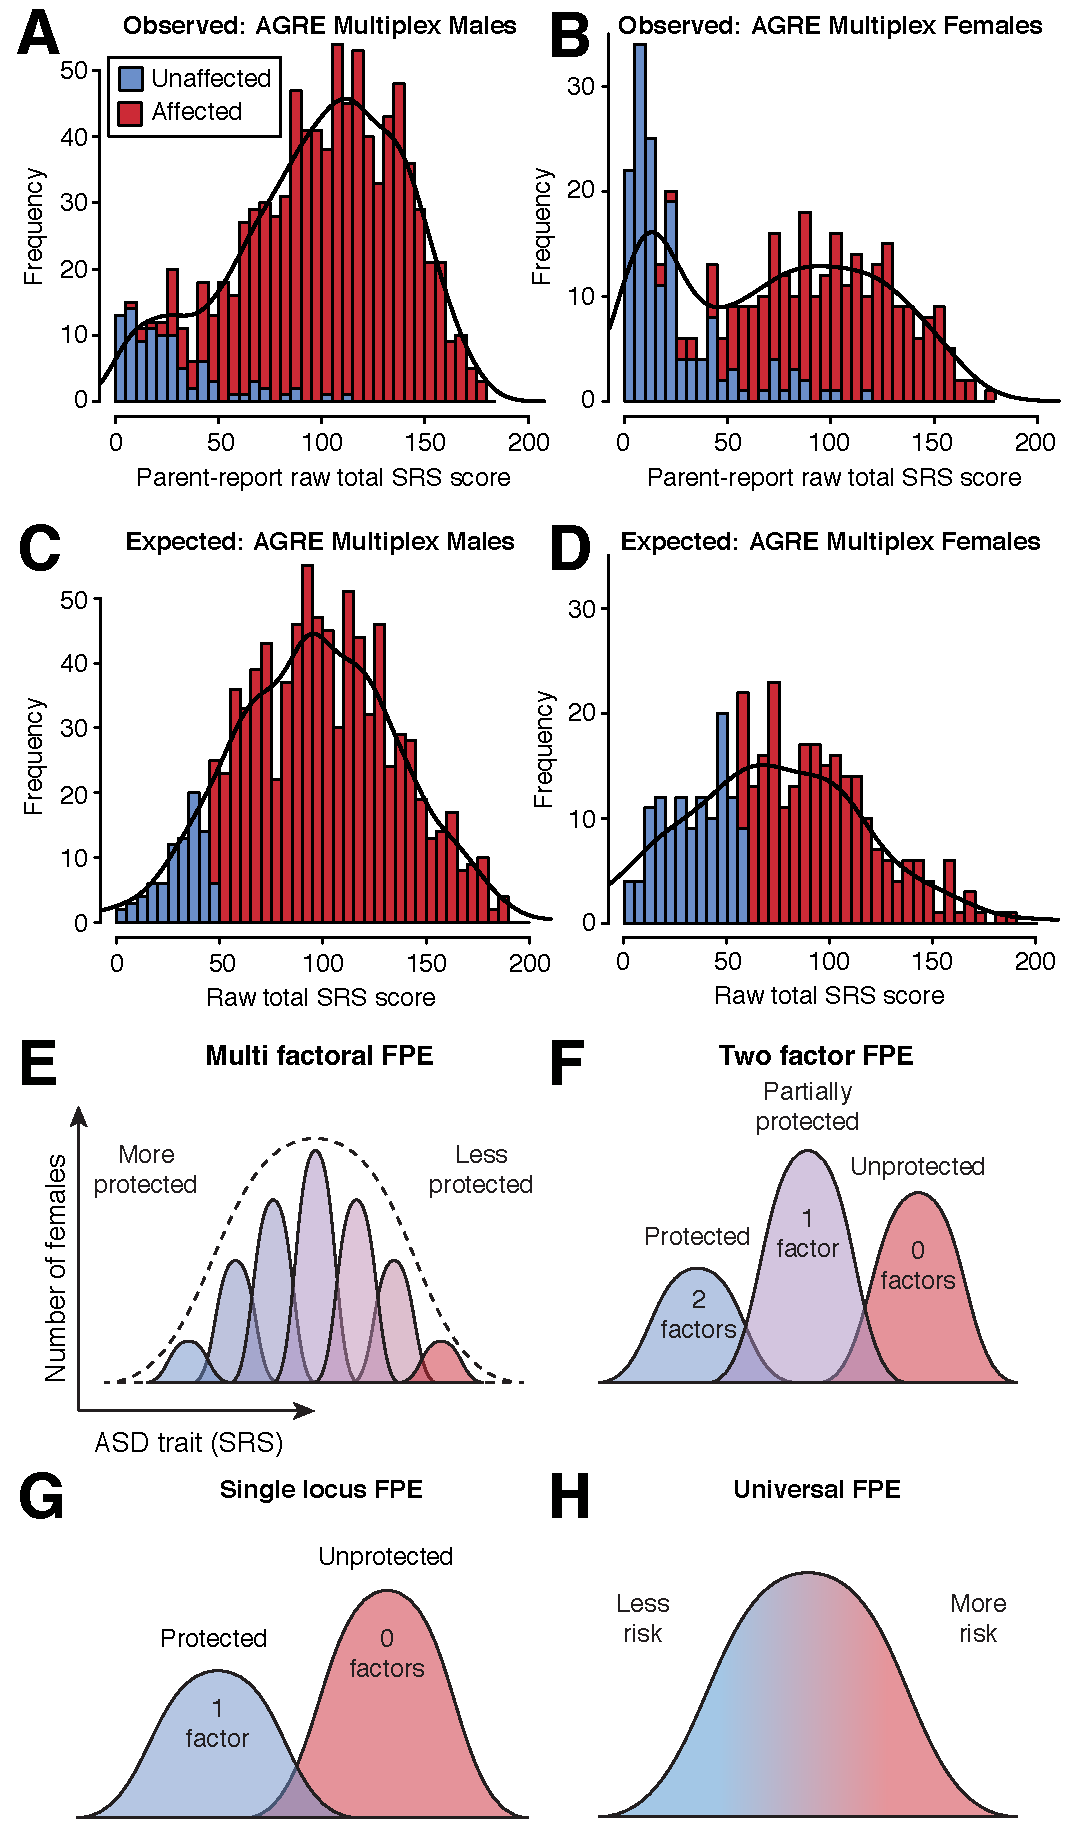
\includegraphics[width=.6\textwidth]{Figures/Figure_1_SRS_Gockley_Dec2014.pdf}
        \caption{\textbf{Expected and Observed Social Responsiveness Scale (SRS) Scores in Multiplex AGRE Families.}  			\label{Figure1}}     	
       		\scriptsize\begin{flushleft}Children in multiplex families are assumed to have inherited a high degree of ASD risk. Under a threshold model, a quantitative measure of ASD severity, such as the SRS, would be expected to follow a normal distribution with unaffected individuals at the lower end. \textbf{A)} The observed SRS scores for 927 male children (95 unaffected in blue, 832 affected in red) with each bar showing the sum of the number of unaffected and affected males. The black line shows the kernel density of the data, which approximates a normal distribution. \textbf{B)} The corresponding plot is shown for 394 female children (151 unaffected, 243 affected). The SRS scores produce a bimodal distribution, as noted previously \cite{Constantino:2010aa,Virkud:2009aa}. \textbf{C)} To assess the expected distribution under quantitative trait model the mean and standard deviation of the male observed data was estimated (A) and used these characteristics to simulate a normal distribution for the same number of individuals. The scores were sorted and a threshold for affected status was chosen to give the same number of affected and unaffected males as in ‘A’. Each bar shows the sum of the number of unaffected and affected simulated males, while the black line shows the kernel density. \textbf{D)} The expected distribution under quantitative trait model is shown using the same method as in ‘C’ but for 394 females based on the female data in ‘B’. The expected distribution differs markedly from the observed in females, but not in males. \textbf{E)} If multiple factors contribute to the presence of the FPE then their combined effect is likely to produce a unimodal distribution. \textbf{F)} As the number of factors contributing to the presence of the FPE decreases, the unimodal distribution in ‘E’ develops distinct distributions based on the number of factors present. \textbf{G)} If only one factor contributes, then a bimodal distribution should be observed. \textbf{H)} Finally, if there are no factors and the FPE is universally present in females a unimodal distribution will arise based on the distribution of risk rather than protection. 
       		\end{flushleft}
	\end{figure}
	\clearpage
}\normalsize
    
    \afterpage{
        \begin{figure}[h!]
			\centering
			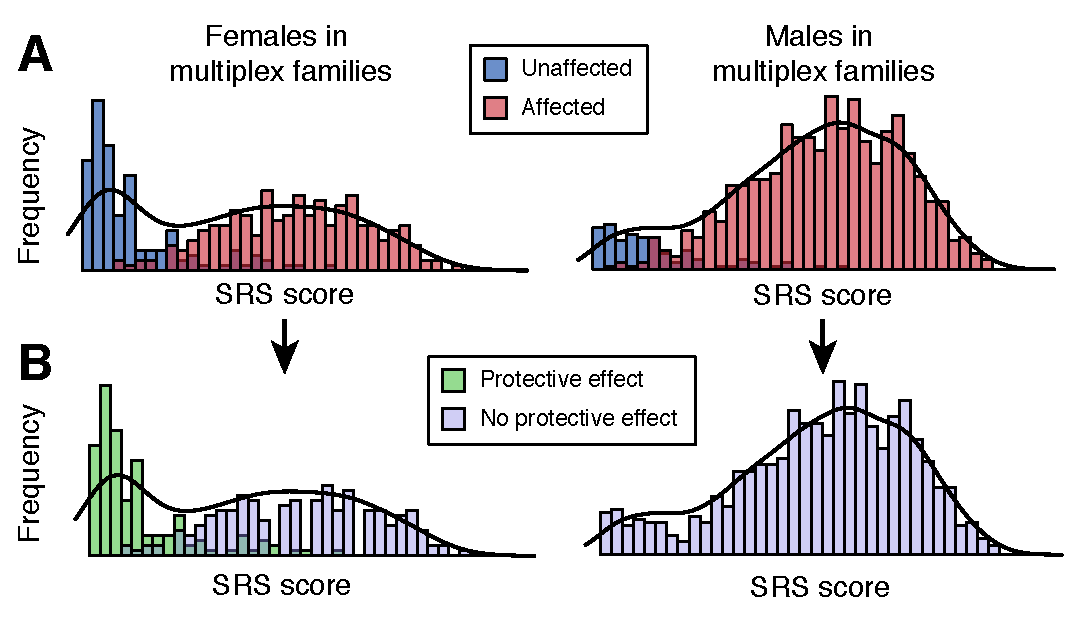
\includegraphics[width=\linewidth]{Figures/Sup_Hypothesis_v3.pdf}
			%\end{center}
			\caption{\textbf{A Single Locus Hypothesis for the Female Protective Effect.}}
			\label{Figure2}
       		\scriptsize\begin{flushleft}\textbf{A)} A bimodal distribution of ASD risk, measured with the SRS, is observed for females from multiplex families but is less distinct in males. \textbf{B)} This bimodal distribution may reflect females with a protective effect (in green) vs. females without such a protective effect (in purple). 
       		\end{flushleft}
	\end{figure}
    \clearpage
	}\normalsize
	
\afterpage{
	\begin{figure}[h!]
		\centering 
			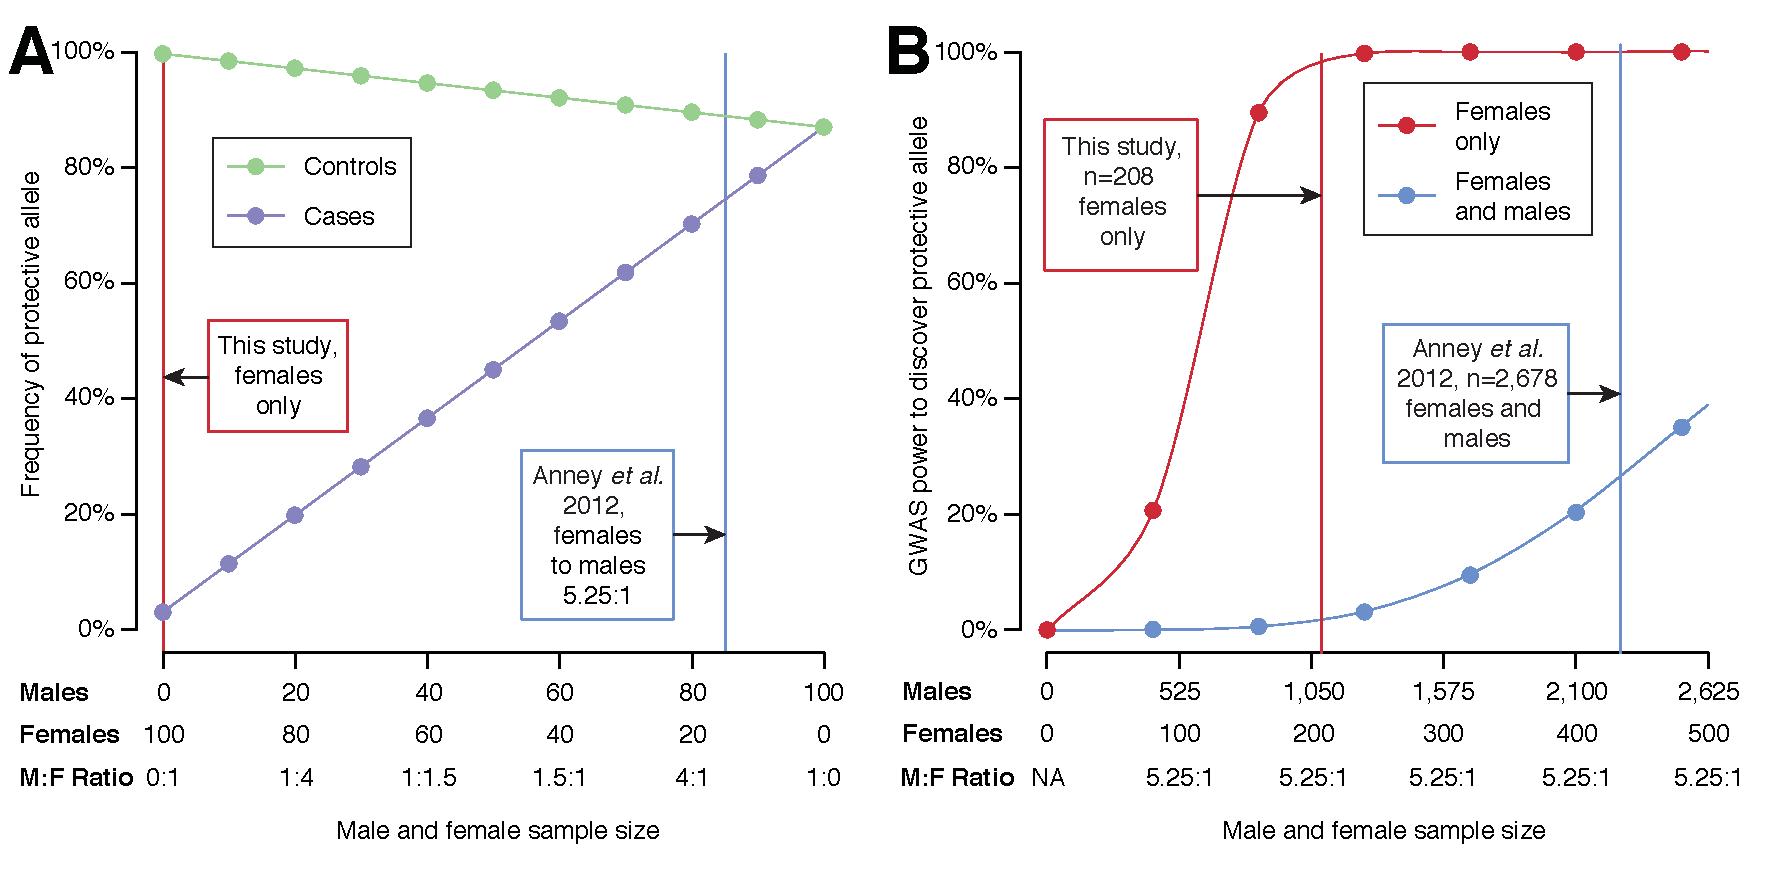
\includegraphics[width=\linewidth]{Figures/Figure_2_Power_Gockley_Dec2014.pdf}
		%\end{center}
		\caption{\textbf{GWAS Power Estimate for a Single Factor Mediating the FPE. }}
		\label{Figure3}
       		\scriptsize\begin{flushleft}\textbf{A)} In females exposed to high ASD risk the protective factor will be enriched in unaffected individuals (green) and largely absent in cases (purple). A distinct difference in the frequency of the protective allele in these two cohorts can be estimated for an analysis based only on females (red line). Conversely, the protective allele has no effect in males and will be observed at an equal frequency in male cases and controls. Including males in a GWAS analysis will therefore add noise (blue line, representing the observed 5.25:1 ratio of males to females in Anney et al. 2012) resulting in a reduction in power. \textbf{B)} An estimate of GWAS power to detect a single FPE allele in females only (red) and females and males (blue) under a model where protection contributes 50\% of the observed 5.25:1 sex bias. The vertical lines represent the sample size in this study (red) and the \cite{Anney:2012aa} GWAS study (blue).
       		\end{flushleft}
	\end{figure}
    \clearpage
}\normalsize

\afterpage{
        \begin{figure}[h!]
			\centering
			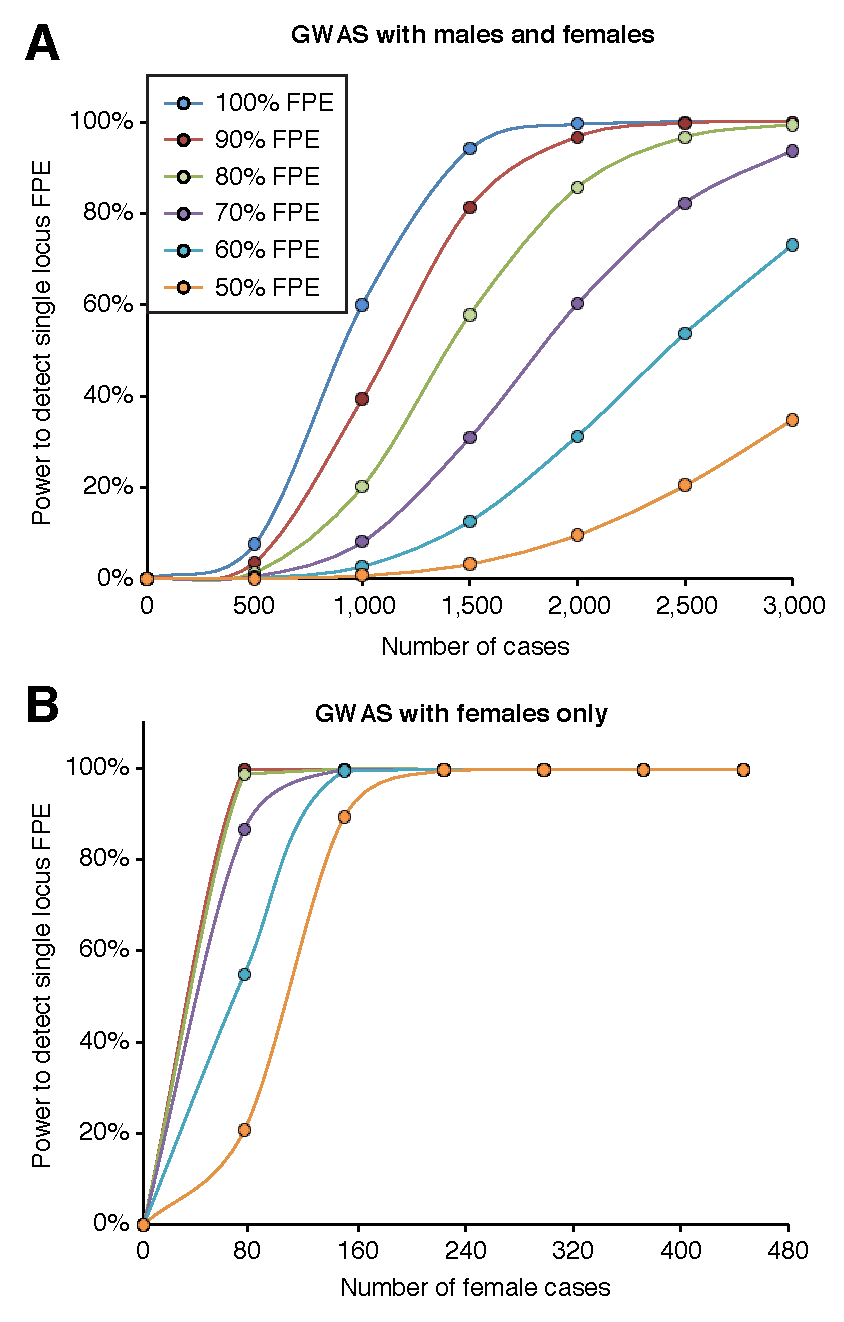
\includegraphics[width=.6\linewidth]{Figures/Power_Supp.pdf}
			%\end{center}
			\caption{\textbf{Power to Detect a Single Locus FPE.}}
			\label{Figure4}
       		\scriptsize\begin{flushleft}\textbf{A)} Power was estimated based of the predicated allele frequencies (Table \ref{Table1}) in affected females vs. population females. To model deviation from ideal conditions, the contribution of the FPE to ASD sex bias was decreased from 100\% to 50\%. For a given number of cases, and an equivalent number of controls, the estimated power is shown. For comparison, the largest GWAS in ASD used 2,678 cases and pseudo-controls \cite{Anney:2012aa}. \textbf{B)} The analysis is repeated for females only, based on the observed rate of 16\% \cite{Anney:2012aa}. The power is consistently greater in this female only analysis than in a conventional GWAS.
       		\end{flushleft}
	\end{figure}
    \clearpage
}\normalsize
    
\afterpage{    
  	\begin{table}[h!]
		\renewcommand{\arraystretch}{1.1}
		\centering
			\begin{tabular}{|l|c|c|c|c|c|}

			\hline 
			\textbf{Category} & \textbf{PP} & \textbf{Pp} & \textbf{pP} & \textbf{pp} \\ \hline 
			Frequency in females & 75.69\% & 11.31\% & 11.31\% & 1.69\% \\ \hline 
			Frequency in affected females & 3.02\% & 45.12\% & 45.12\% & 6.74\% \\ \hline 
			Frequency in unaffected females & 99.68\% & 0.15\% & 0.15\% & 0.02\% \\ \hline 
			\end{tabular}
	
		\caption{\textbf{Predicted Frequency of p Risk Allele Under a Dominant Model in Cases and Controls}}
		\label{Table1}
		%\end{center}
The ``Frequency in females'' of each genotype is estimated from a \textit{P} allele frequency of 87\% and a \textit{p} allele frequency of 13\%. Under a model where the FPE reduces the incidence of ASD by 100-fold, the \textit{PP} genotype is markedly reduced in affected females. Conversely, if all females have been exposed to risk, as expected in a multiplex family, the unaffected females should be depleted for non-protective genotypes. For power calculations (Figure \ref{Figure4}) the more conservative estimate of ``Frequency in females'' was used to estimate allele frequency in unaffected females, rather than the ``Frequency in unaffected females''.
	\end{table}  
	\clearpage
}\normalsize
        
\afterpage{
      \begin{figure}[h!]
			\centering 
			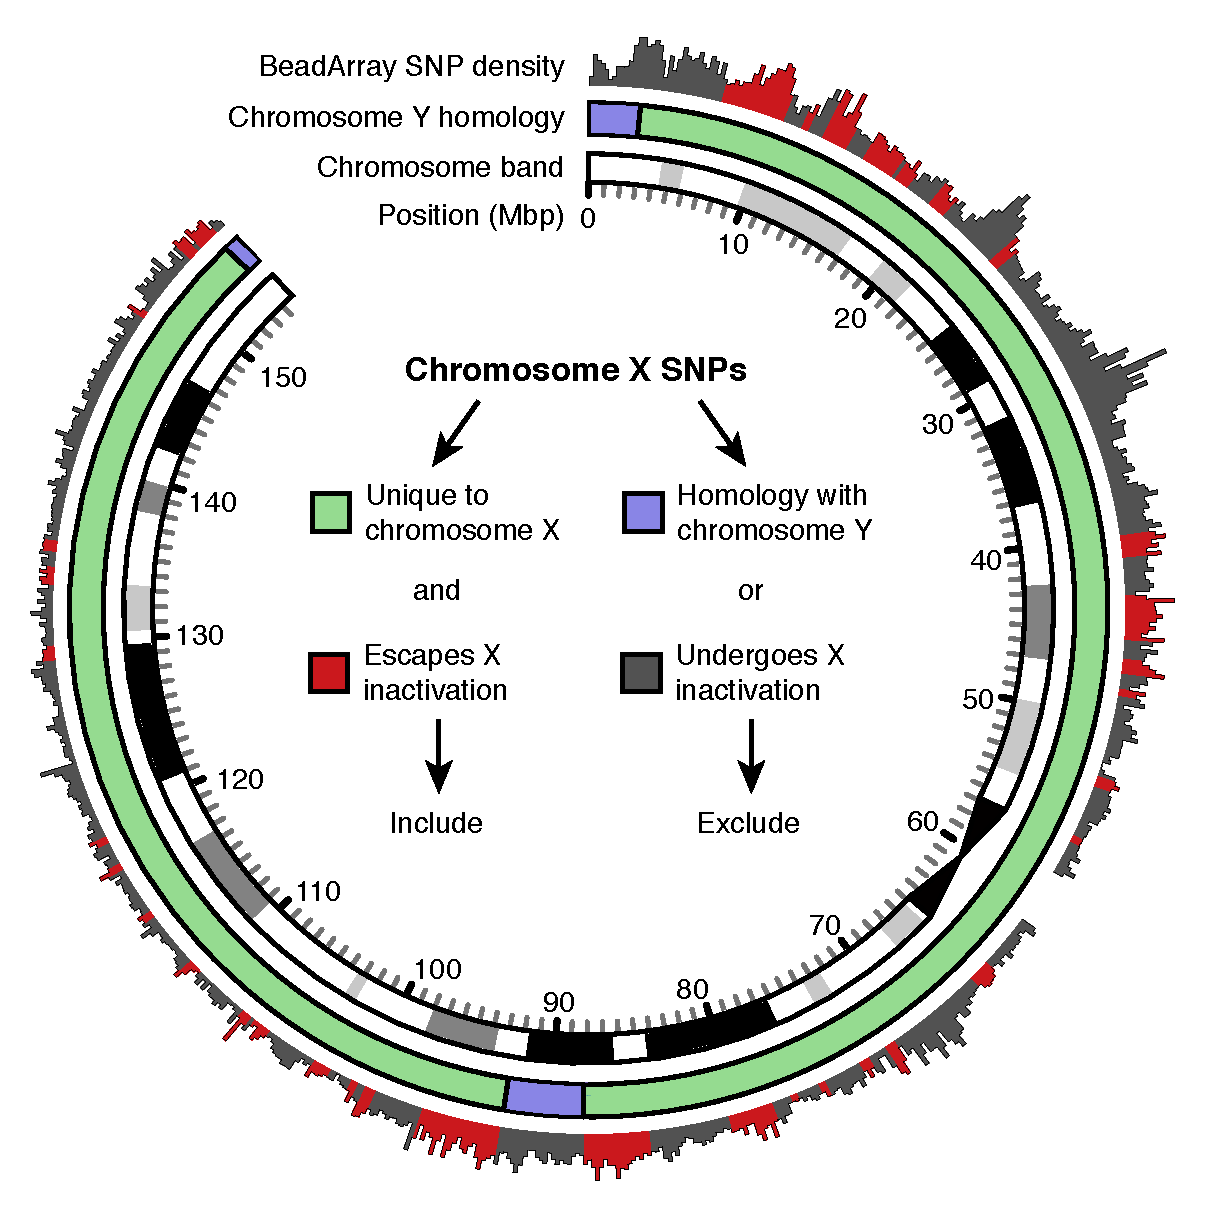
\includegraphics[width=1\linewidth]{Figures/Figure_3_Circos_Gockley_Dec2014.pdf}
			\caption{\textbf{Identification of Chromosome X SNPs that Escape X-Inactivation for Tier 1 Analysis.}}
			\label{Figure5}
       		\scriptsize\begin{flushleft}This Circos plot shows the length of chromosome X proceeding clockwise with position 0 on the short arm at twelve o’clock. Adjacent to the chromosome position, the innermost ring indicates chromosome banding by the depth of shading; two opposing black arrows indicate the centromere. Regions of chromosome Y homology are shown in purple in the middle ring; SNPs in these regions were excluded from the tier 1 analysis leaving the SNPs unique to chromosome X indicated in green. The outermost ring shows SNP density based on the genotyping array (See Methods) by the height of the bars. Regions that are inactivated on one copy of chromosome X are shown in grey \cite{Carrel:2005aa} and SNPs in these regions were excluded from the tier 1 analysis, leaving only SNPs that escape X-inactivation, shown in red (Table \ref{Table1A}). Of the 6,955 SNPs on chromosome X, 451 (6.5\%) were included in the tier 1 analysis.
       		\end{flushleft}
            %\end{center}
	\end{figure}
    \clearpage
}\normalsize    
    
	
    \section{Methods}
    	
        \subsection{Subjects and Genotyping}
			Genotyping data were collated from two independent large cohorts of ASD families: 1,976 families from the Autism Genome Resource Exchange (AGRE) \cite{Geschwind:2001aa} and 2,733 families from the Simons Simplex Collection (SSC) \cite{Fischbach:2010aa}. The AGRE data were generated on one of three Illumina Bead Arrays: 550v1 (421 families), 550v3 (1,277 families), and Omni 1M (278 families). Analysis was restricted to the 329,483 SNPs shared between all three arrays. The SSC data were generated on one of three Illumina Bead Arrays: 1Mv1 (421 families), 1Mv3 Duo (1,277 Families), and Omni 2.5M (1,035 Families). Analysis was restricted to the 493,924 SNPs shared between all three arrays.

	\subsection{Ancestry and data cleaning}
    	Ancestry was examined as described in \cite{Anderson:2010aa}. Briefly, founders from the HapMap CEU, CHB, JPT, and YRI ancestral populations were used to train the model \cite{Duan:2008aa}. Common SNPs between all four populations and the AGRE or SSC cohort were identified in plink. Alleles were forced to the same strand, A$\to$T and G$\to$C SNPs were excluded because of alignment concerns. The final dataset was analyzed utilizing EIGENSTRAT \cite{Price:2006aa}. Samples of European ancestry in the AGRE and SSC cohort were determined by deviation in PCA components 1 and 2 between the AGRE or SSC samples and the HapMap CEU individuals. In order to be classified as European, a cohort individual was required to have a PCA component 1 and PCA component 2 value within 1.5 standard deviations of the HapMap CEU PCA component 1 and 2 means (Figure \ref{Figure6}). 
       \par Data were restricted to families of European ancestry and standard GWAS data cleaning were performed. European ancestry was determined using Eigenstrat \cite{Li:2008aa} and the four core HapMap populations Figure \ref{Figure6} [30]. The resulting genomic inflation for European samples was 1.03 Figure \ref{Figure6}. SNP data were cleaned using PLINK \cite{Purcell:2007aa}, specifically: minor allele frequency ≥0.03 (Supplementary Methods); genotype rate of ≥0.95 per sample (minimum observed genotyping rate was 0.991); genotype missingness per SNP $\leq$ 0.1; Hardy-Weinberg Equilibrium $<$ 0.0001. After data cleaning there were 943 families and 317,574 SNPs for AGRE and 2,166 families and 440,778 SNPs for SSC.

\subsection{Identifying Unrelated Females Through Identity by Descent}
        Of the 943 remaining AGRE families, only 510 contained at least one female with genotyping data. Where a family had multiple females only one was selected, with a preference for unaffected females, since these are less frequent in the AGRE sample. From these, 151 unaffected females and 208 affected females (defined as “Autism” or “Broad Spectrum”) were identified and used for the analysis. Identity by descent demonstrated that these samples were all unrelated, Figure \ref{Figure7}.
\par A similar approach was applied to the 2,166 remaining SSC families, of which 883 had at least one female. In families with multiple females only one was selected, with a preference for affected females, since these are less frequent in the SSC sample. The analysis was therefore performed on 207 affected females and 676 unaffected females.

	\subsection{Defining Regions Which Escape X-inactivation \& SNPs of interest}
    	For the first tier of analysis, SNPs on chromosome X were selected if they lacked homology to chromosome Y and escaped X-inactivation (Figure \ref{Figure5}, \ref{Table1A})\cite{Carrel:2005aa}. These regions represent 14\% of chromosome X (21.8Mbp). This left 451 SNPs for analysis in the AGRE data and 720 SNPs in the SSC data. For the second tier analysis all of chromosome X was considered with 6,955 SNPs in AGRE and 10,269 SNPs in SSC. Finally, for the third tier of analysis all SNPs that remained after cleaning were included with 317,574 SNPs in AGRE and 440,778 SNPs in SSC.
        Regions that escape X inactivation were determined according to the results of a gene-based rodent/human somatic cell hybrid study \cite{Carrel:2005aa}. Nine hybridomas were assessed. If gene expression was observed from an inactivated human X chromosome in at least three hybridomas, that gene was considered to escape X-inactivation. To identify regions, rather than genes, regions between consecutive escaping genes were also defined as escaping X inactivation. The co-ordinates used were defined by the first gene start position and last gene stop position plus 1kbp at either end to include regulatory regions in close proximity. UCSC gene definitions and hg18 genomic co-ordinates were used throughout (Figure \ref{Figure5}, Table \ref{Table1A}).        
        
    \subsection{Hypothesized Allele Testing}
    	All analyses presented in this section are based on the hypothesis that a single common allele is responsible for a female protective effect (FPE) that produces a 4:1 sex bias in autism. There are three variables that constrain the allele frequency for such an allele: 1) The incidence of autism in the population, this assumes an estimate of 1\% \cite{Fombonne:2009aa}; 2) The observed sex bias, will use an estimate of 4:1 male to female \cite{Fombonne:2009aa}; and 3) the effect of the FPE on the incidence of ASD. The hypothesis states that the FPE is unevenly distributed between females, being present in some, but absent in others, however there is no known empirical evidence regarding how effective such protection might be under this hypothesis. Therefore, for the purposes of modeling, it is assumed that the FPE was highly effective in protecting against ASD, using an arbitrary estimate of a 100-fold reduction in risk. 

	For consistency across the different tiers of the analysis, a protective major allele (\textit{P}) and a non-protective minor allele (\textit{p}) was considered with \textit{p} acting in a dominant fashion to disrupt protection. Of note, the power calculations are unchanged if the non-protective allele acted in a recessive fashion, as the predicted difference in allele frequency between cases and controls is identical. 

	Under a dominant model, \textit{PP} confers protection, while \textit{Pp}, \textit{pP}, and \textit{pp} do not. To produce a 4:1 sex bias and 1\% ASD incidence, the \textit{P} allele must occur at a population frequency of 87\% (see Table \ref{Table2}). Under this hypothesis 76\% (87\% x 87\%) of females are protected, while the remaining 24\% lack protection.
    
	Under a model where the FPE reduces ASD incidence by 100-fold, affected females would be expected to be greatly depleted for the protective \textit{PP} genotype. Table \ref{Table3} shows the estimated percentage of females with two copies of the \textit{P} allele in the affected group and in the unaffected group, assuming all unaffected females were exposed to risk. Since only females are considered in all three tiers of the association analysis, these estimated frequencies will not change regardless of whether chromosome X or autosomes are considered.  
    
    Association tests were performed using PLINK\cite{Purcell:2007aa} under a dominant model. All p-values were corrected for multiple comparisons, using Bonferroni correction based on the number of SNPs analyzed in each tier. The cluster plots of all SNPs highlighted by the analysis are shown in Appendix \ref{AppendixC}.
    
    \subsection{Power Calculation}
 		Having estimated the frequency of the \textit{PP} genotype in affected females, the ability to detect these alleles in an association study was considered. The estimate of allele frequencies in unaffected females (Table \ref{Table3}) assumes that these subjects were exposed to risk, however this probably not the case for a subset of females due to \textit{de novo} mutations and rare inherited variants acting in a dominant manner. Therefore, the \textit{PP} genotype frequency in the population (Table \ref{Table3}, ``Frequency in females'') represents a worst case (no enrichment of unprotected females) while the \textit{PP} genotype frequency in unaffected females (Table \ref{Table3}, ``Frequency in unaffected females'') is a best case scenario. For the purposes of the power estimation, we used the population \textit{PP} genotype frequency as the more conservative approach.

		Power was estimated using G*Power3.1 \cite{Faul:2007aa} using the ``exact'' test family, ``Proportions: Inequality, two independent groups (Fisher's exact test)'', ``Post hoc: Compute achieved power - given $\alpha$, sample size, and effect size''. For power of a GWAS, two tailed analysis was selected, the frequency of the \textit{PP} genotype in affected females was entered as ``Proportion p1'' and the proportion of the \textit{PP} genotype in unaffected females was entered as ``Proportion p2''. The value used for ``$\alpha$ err prob'' was 1e-07. For sample size of each group, the number of cases and controls used was equal (in line with the pseudo-controls used)\cite{Anney:2012aa}. The results are shown in Figure \ref{Figure4}.

		This model assumes that: 1) The FPE is solely responsible for the 4:1 sex bias; 2) The hypothesized locus is solely responsible for the FPE; 3) ASD diagnosis is 100\% accurate in assessing cumulative ASD risk; and 4) The FPE reduces incidence by 100-fold. There is a high likelihood that the population effects differ from one or more of these assumptions; therefore how statistical power is affected by deviation from this model was assessed. To achieve this, the extent to which the FPE contributed to ASD sex bias was reduced. To consider a model where the FPE only contributed 50\% of sex bias, the difference between the frequency of the \textit{p} risk allele in affected and unaffected females (97\% - 24\% = 73\%) was halved (73\% / 2 = 36.5\%) and the new \textit{p} risk allele frequency in affected females was calculated by adding this difference to the \textit{p} risk allele frequency in unaffected females (24\% + 36.5\% = 60.5\%). The power calculation was repeated with this lower estimate of the \textit{p} risk allele in affected females. The results of reducing the FPE contribution are shown in Figure \ref{Figure4}.

		Reducing the contribution of the FPE to ASD sex bias is a method of testing the relative power of a conventional GWAS versus a sex-specific GWAS for this hypothesis. The decreasing contribution of the FPE can be considered as a proxy for adding noise or general deviation from the optimal predicted conditions. Of note, the sex-specific GWAS achieves considerably greater power for an equivalent sample size than a conventional GWAS (Figure \ref{Figure4}). 
 
	\subsection{SRS Based Subject Groupings of Females in Multiplex Autism Families}
 		
        It was considered that the possibility of females with and without protection may be best defined by considering SRS scores instead, or in combination, with ASD affected and unaffected diagnosis. The first exploratory analysis was based purely on parent SRS score and identified a high SRS `case' group and a low SRS `control' group (Figure \ref{Figure2}); sample sizes are based on females with high quality data and European ancestry who were used in the analysis (Table \ref{Appendix2FPEsamp}); \textbf{High SRS}: SRS $>$45, N=103 in AGRE; N=198 in SSC, \textbf{Low SRS} SRS: $\le$45, N=74 in AGRE; N=621 in SSC. No SNPs reached significance after correcting for multiple comparisons in this analysis (Figure \ref{Figure8}, \ref{Figure9}, \ref{Figure10}, \ref{Figure11}, \ref{Figure12}, \ref{Figure13} and Table \ref{Table4}).
 
 	Since AGRE is a multiplex collection, the majority of individuals are likely to carry a high burden of ASD genetic risk compared with the general population. To identify a subset of females likely to be enriched for the protective allele; first, females were classified as being affected or unaffected. Then females were further stratified within each diagnostic group by their SRS score to identify four cohorts (Figure \ref{Figure14}); sample sizes are based on samples with high quality data and European ancestry who were used in the analysis: \textbf{Affected, high SRS} (upper 50\% of all affected females; N=58 in AGRE), \textbf{Affected, low SRS} (lower 50\% of all affected females; N=51 in AGRE) \textbf{Unaffected, high SRS} (SRS $>$45; N=54 in AGRE) \textbf{Unaffected, low SRS} (SRS $\le$45; N=64 in AGRE). 
    
   Exploratory association analyses were performed with alternative definitions of the protected and unprotected groupings of females: Affected, high SRS (unprotected) vs Affected, low SRS (protected), Affected, high SRS (unprotected) vs Unaffected, high SRS (protected), Affected, high SRS (unprotected) vs Unaffected, low SRS (protected), Affected, low SRS (unprotected) vs Unaffected, high SRS (protected), Affected, low SRS (unprotected) vs Unaffected, low SRS (protected), Unaffected, high SRS (unprotected) vs Unaffected, low SRS (protected).  
 
	 None of these analyses produced SNPs with p-values exceeding the significance threshold after correction for multiple SNP comparisons (Table \ref{Table4}). Given the exploratory nature of this analysis data was not corrected for the multiple association tests.
     
     \subsection{Assessing the Impact of Ascertainment Bias on Liability}
     
     The multiplex families used in AGRE for the initial observation of a bimodal SRS distribution in females were selected on the basis of having two children affected with ASD. To assess the impact of this ascertainment bias on the distribution of ASD liability a simulation was developed.

	A male and female parent were assigned a random value for ASD liability based on a standard normal distribution (mean=0, SD=1). To model the female protective effect the mean liability in males was increased by 0.33 standard deviations and decreased by the same factor in females. These values produced a 4:1 sex bias. A diagnostic z-score threshold of 2.93 was set to produce an incidence of 1\%. 

	The mean liability of the two parents was estimated and this mean was used to estimate a random value for the ASD liability of two male children and two female children. As with the parents, the male mean was increased by 0.33, while the female mean was decreased by the same factor. If two children in the family exceeded the diagnostic threshold the family was included and the liability estimates returned.

	1 million families were simulated and the liability distribution of the male and female children were plotted (Figure \ref{Figure15}A and \ref{Figure15}B). The resulting distribution was made up of two overlapping distributions: 1) the tail end of the normal distribution cut-off at the diagnostic threshold representing the children that contributed to the ascertainment; and 2) a normal distribution with a mean above the population mean, but below the diagnostic threshold representing the children in ascertained families that did not contribute to ascertainment.

	With the addition of noise, as would be expected using a proxy measure such as the SRS, the female distribution is likely to appear bimodal while the male would be unimodal. However, this does not reproduce the initial observation of a bimodal SRS in multiplex females in two important respects: 

	\begin{enumerate}
	\item For the lower distribution in females the mean is at least one standard deviation above the population (\ref{Figure15}B), however for the SRS distribution in females the SRS scores were comparable to the normal population.

	\item The difference in male and female SRS distributions in the general population is 3 points, equivalent to 0.17 standard deviations. This is four-fold less than the difference in male and female mean used in the simulation shown in Figures \ref{Figure15}A and 	\ref{Figure15}B. Using the 0.17 standard deviation value results in the distributions shown in Figure \ref{Figure15}C and \ref{Figure15}D in which the distributions are similar between the sexes.
\end{enumerate}

	Therefore, while ascertainment bias may partially explain the bimodal SRS in multiplex females it is far from a complete explanation of this phenomena.
     
 %%Ancestry 
	\afterpage{
	\begin{figure}[h!]
		\begin{center}
			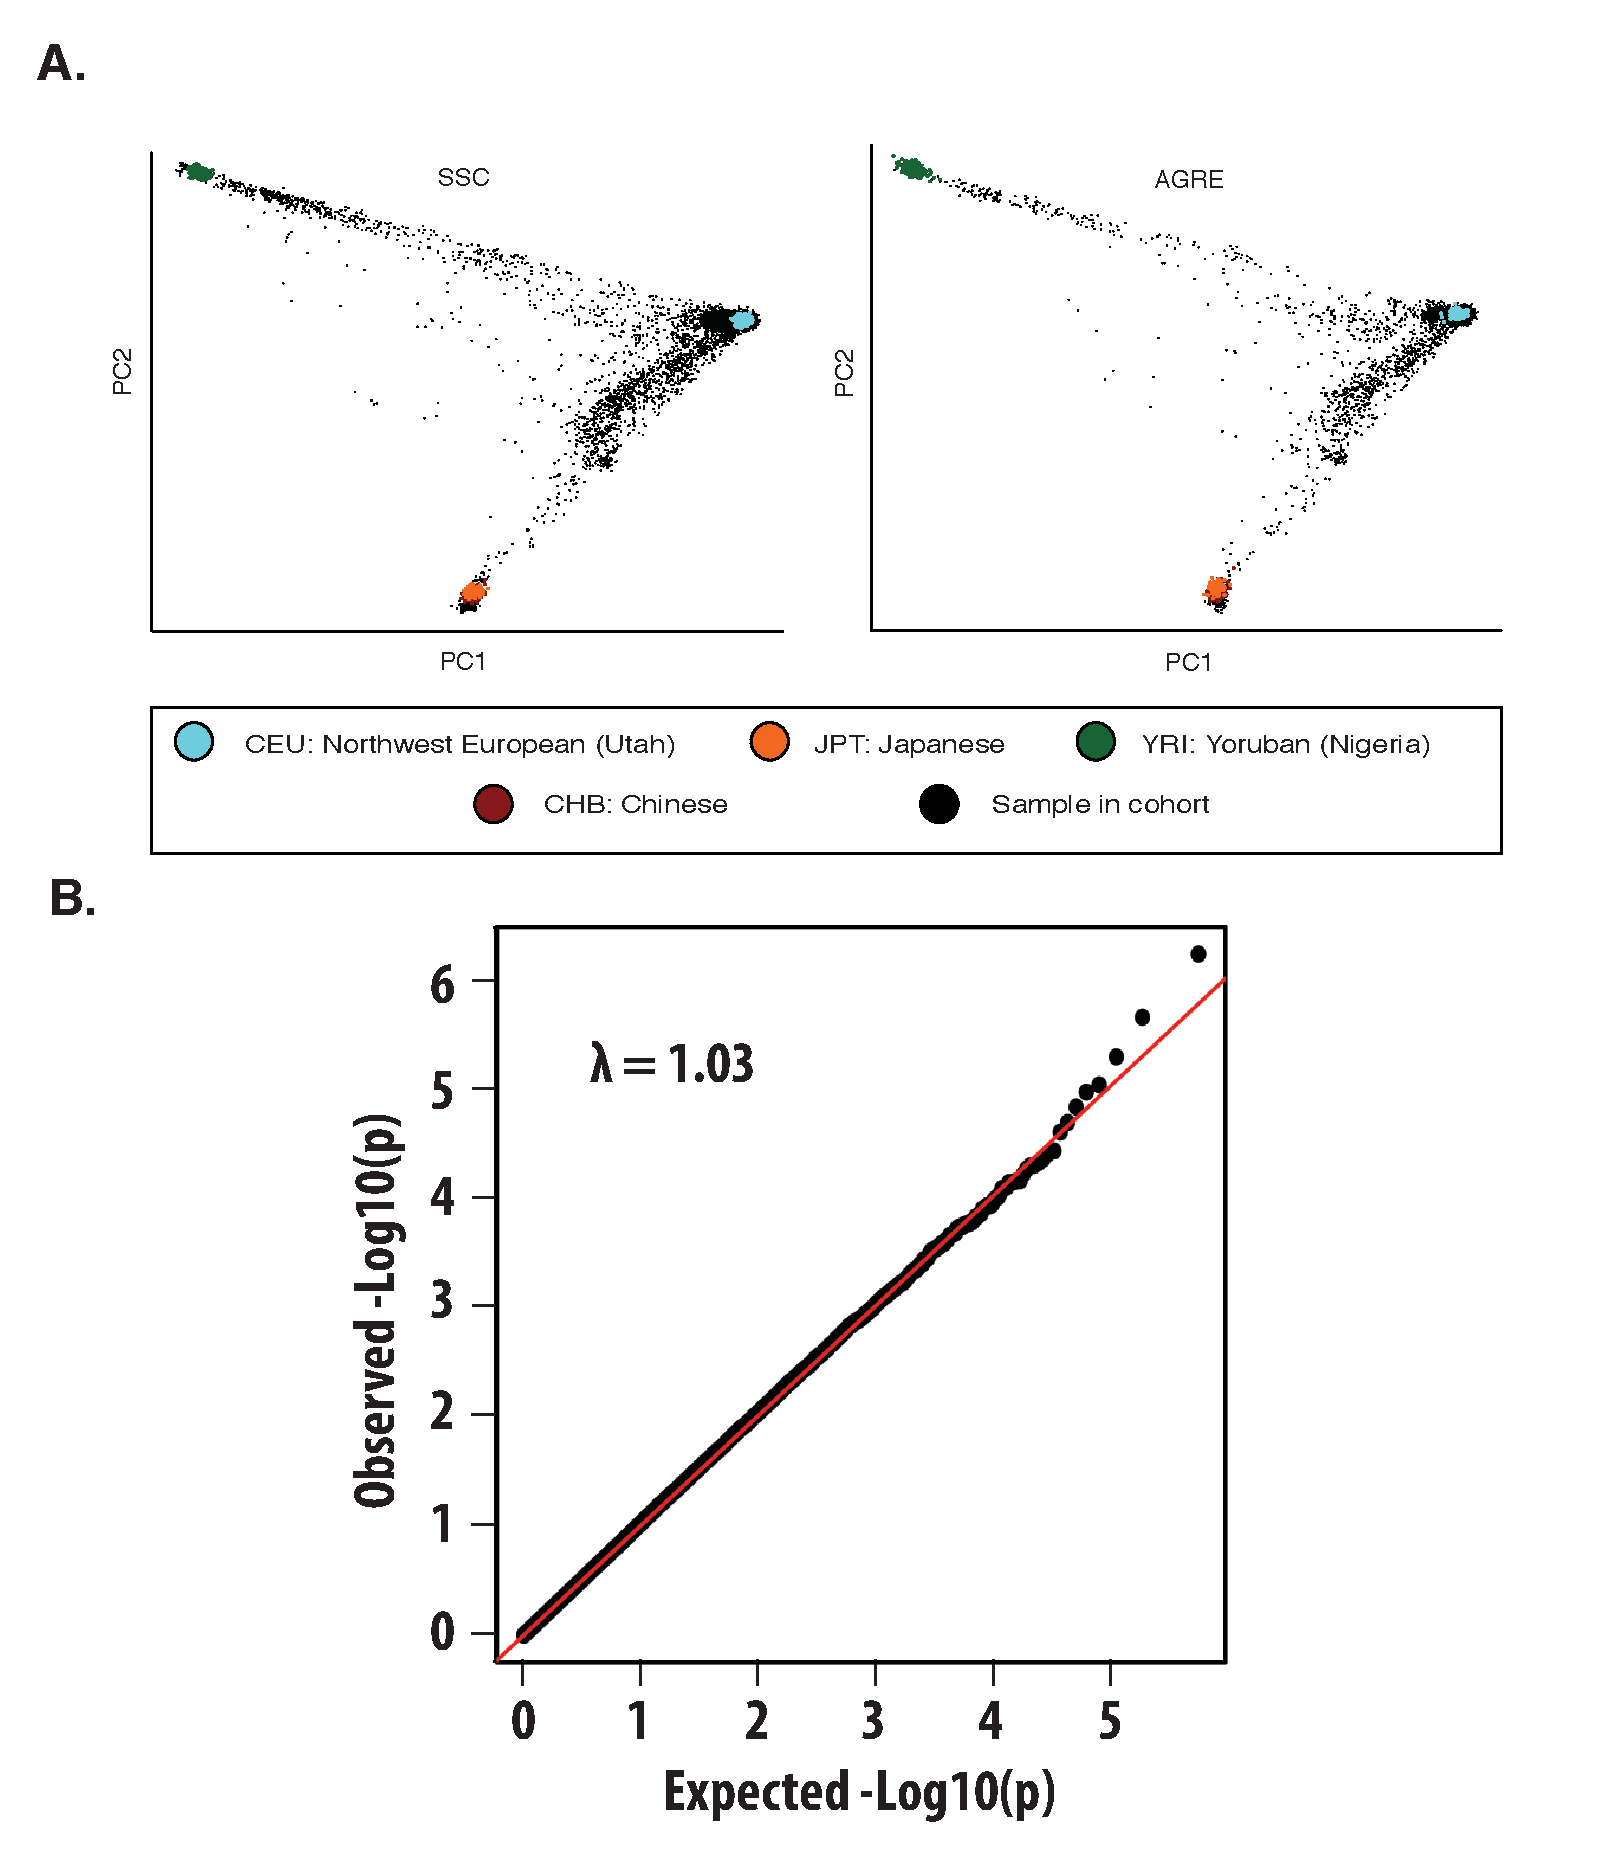
\includegraphics[width=0.9\linewidth, height=5.5in, keepaspectratio=TRUE]{Sup_Figure_2_v2.pdf}
		\end{center}
	\caption{\textbf{Ancestry Analysis.}}
	\label{Figure6}
	\textbf{A)} Population stratification was preformed in EIGENSTRAT. HapMap samples CEU (blue), YRI (green), JPT (Orange), and CHB (red) were used to stratify the AGRE  and SSC cohort. \textbf{B)} QQ-Plot analysis preformed on a GWAS of AGRE samples yielded a genomic inflation ($\lambda$) of 1.03.
	\end{figure}
	\clearpage
	}\normalsize



        
%%IBD
	\afterpage{
		\begin{figure}[h!]
			\begin{center}
				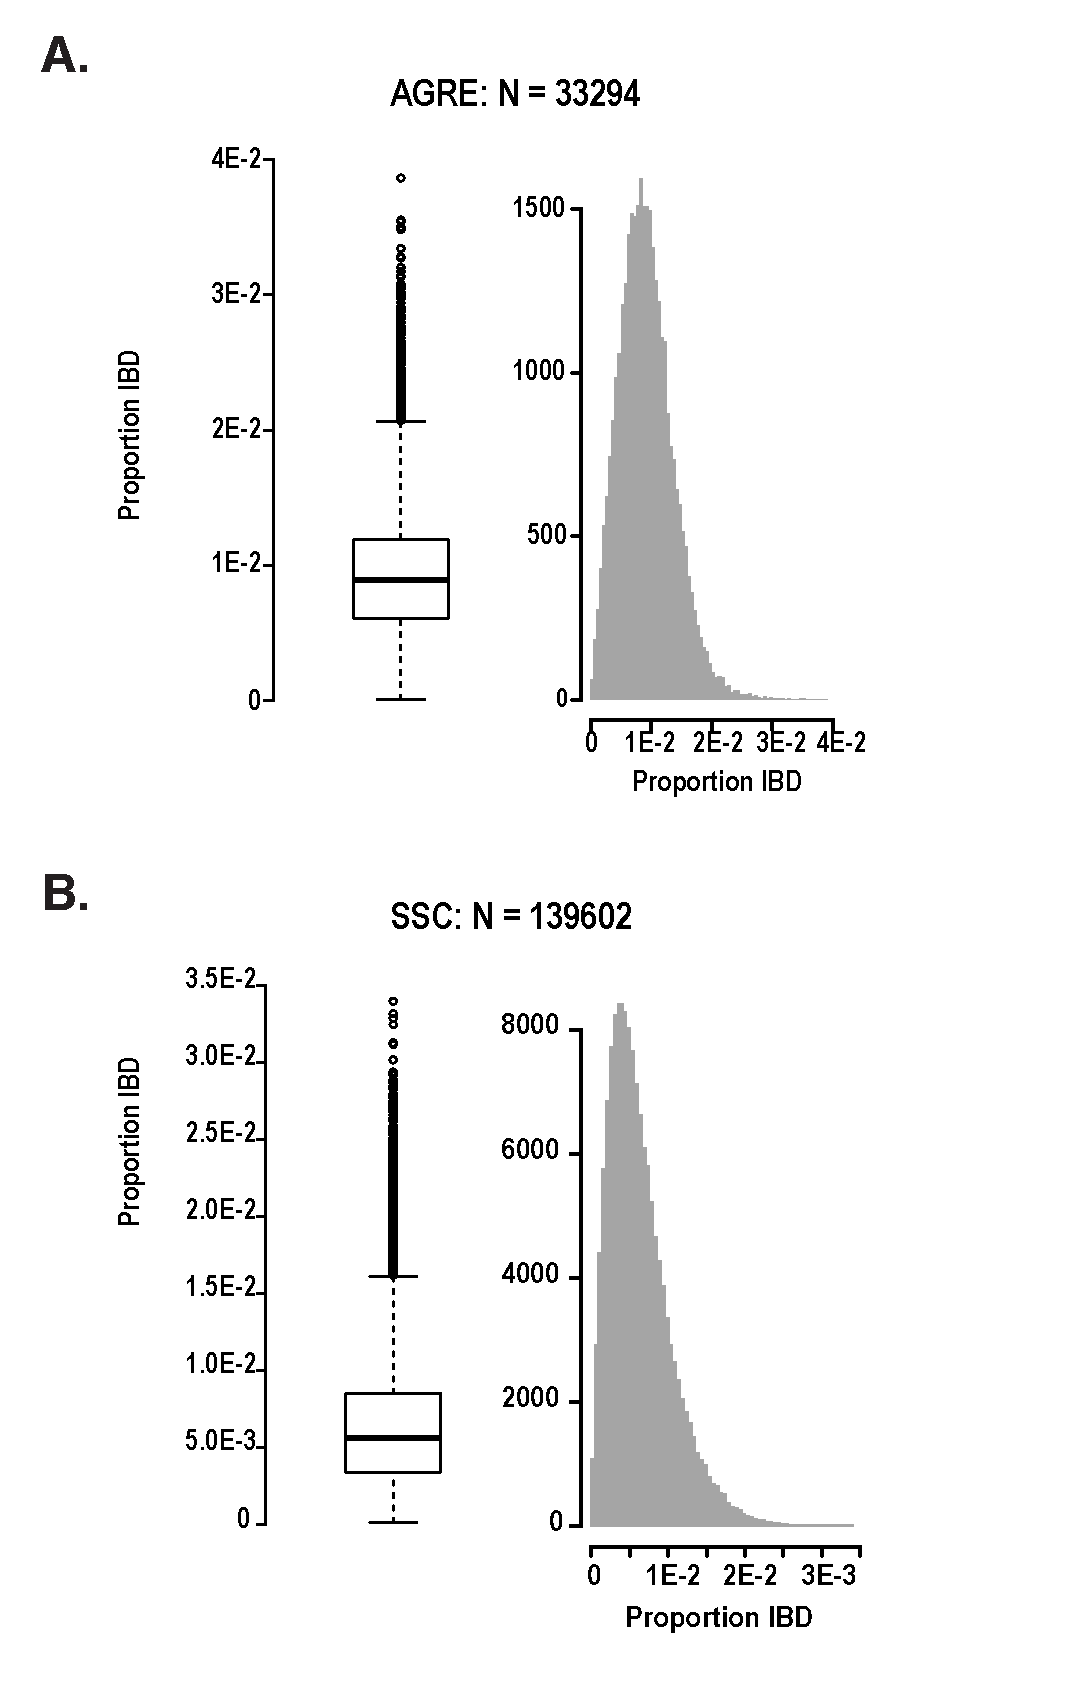
\includegraphics[width=.6\linewidth, keepaspectratio=TRUE]{Sup_Figure_3.pdf}
			\end{center}
			\caption{\textbf{Identity by Descent (IBD) Analysis.}}
			\label{Figure7}
			\textbf{A)} 33,294 (51.8\%) of the pairwise comparisons between samples in the AGRE cohort registered an IBD proportion greater than 0. All pairwise IBD comparisons yielded a value below 4\%. \textbf{B)} 139,602 (35.9\%) of the pairwise comparisons between samples in the SSC cohort registered an IBD proportion greater than 0. All pairwise IBD comparisons yielded a value below 3.5\%.
		\end{figure}       
    \clearpage
	}\normalsize
    
%%Table S2 from paper 
%%Predicted Allele Frequency - Single Locus
\afterpage{
	\begin{table}[h!]
		\renewcommand{\arraystretch}{1.1}
		\begin{center}
			\begin{tabular}{|l|c|c|c|c|c|c|}

				\hline 
				\textbf{Category} & \textbf{PP} & \textbf{Pp} & \textbf{pP} & \textbf{pp} & \textbf{P} & \textbf{p} \\ \hline 
Sex & \multicolumn{4}{|c|}{Female} & \multicolumn{2}{|c|}{Male}  \\ \hline 
Protective effect & Present & \multicolumn{3}{|c|}{Absent} & \multicolumn{2}{|c|}{Absent} \\ \hline 
Population Frequency & 37.8\% & 5.7\% & 5.7\% & 0.8\% & 43.5\% & 6.5\% \\ \hline 
ASD incidence & 0.016\% & 1.6\% & 1.6\% & 1.6\% & 1.6\% & 1.6\% \\ \hline 
Population ASD incidence & 0.006\% & 0.09\% & 0.09\% & 0.01\% & 0.70\% & 0.10\% \\ \hline 
Population ASD incidence & \multicolumn{4}{|c|}{0.20\%} & \multicolumn{2}{|c|}{0.80\%} \\ \hline 
Sex ratio & \multicolumn{4}{|c|}{1.0} & \multicolumn{2}{|c|}{4.0}  \\ \hline 
Total population incidence & \multicolumn{6}{|c|}{1.00\%}  \\ \hline 

			\end{tabular}
			\caption{\textbf{Predicted Allele Frequency of Single Locus FPE}}
			\label{Table2}
		\end{center}
The presence of a simple bimodal distribution raises the possibility that a protective allele (\textit{P}) at a single locus could produce the female protective effect; protection mediated by two copies of the allele (\textit{PP}) would be limited to females. Furthermore, a population allele frequency of 87\% for \textit{P}, and 13\% for the non-protective \textit{p} allele, leads to the observed ASD sex ratio of 4:1. ``Population frequency'' is calculated by: 50\% (percent of population of that sex) x allele 1 frequency x allele 2 frequency. ``ASD incidence'' is estimated based on a total ASD incidence of 1.0\% and an arbitrary 100x reduction in incidence when the female protective effect is present. ``Population ASD incidence'' is estimated by ``Population frequency'' multiplied by ``ASD incidence'' and these are summed to give ``ASD incidence'' by sex and ``Total population incidence''. The ratio of ``ASD incidence'' by sex gives the ``Sex ratio''. A \textit{P} allele frequency of 87\% is the only value to produce a 4:1 sex ratio and 1\% ASD incidence. Decreasing the effectiveness of the FPE from 100-fold requires the allele frequency of \textit{P} to increase.
	\end{table}
	\clearpage
}\normalsize

%%Predicted Allele Frequency - Dominant Model
\afterpage{
	\begin{table}[h!]
		\renewcommand{\arraystretch}{1.1}
		\begin{center}
		\begin{tabular}{|l|c|c|c|c|c|}
			\hline 
			\textbf{Category} & \textbf{PP} & \textbf{Pp} & \textbf{pP} & \textbf{pp} \\ \hline 
Frequency in females & 75.69\% & 11.31\% & 11.31\% & 1.69\% \\ \hline 
Frequency in affected females & 3.02\% & 45.12\% & 45.12\% & 6.74\% \\ \hline 
Frequency in unaffected females & 99.68\% & 0.15\% & 0.15\% & 0.02\% \\ \hline 
		\end{tabular}
		\caption{\textbf{Predicted Frequency of p Risk Allele Under a Dominant Model in Cases and Controls}}
		\label{Table3}
		\end{center}
The ``Frequency in females'' of each genotype is estimated from a \textit{P} allele frequency of 87\% and a \textit{p} allele frequency of 13\%. Under a model where the FPE reduces the incidence of ASD by 100-fold, the \textit{PP} genotype is markedly reduced in affected females. Conversely, if all females have been exposed to risk, as expected in a multiplex family, the unaffected females should be depleted for non-protective genotypes. For power calculations (Figure \ref{fig:power}) the more conservative estimate of ``Frequency in females'' was used to estimate allele frequency in unaffected females, rather than the ``Frequency in unaffected females''.
	\end{table}
    \clearpage
}\normalsize

%%Dominant Model
\afterpage{
	\begin{figure}[h!]
		\begin{center}
			%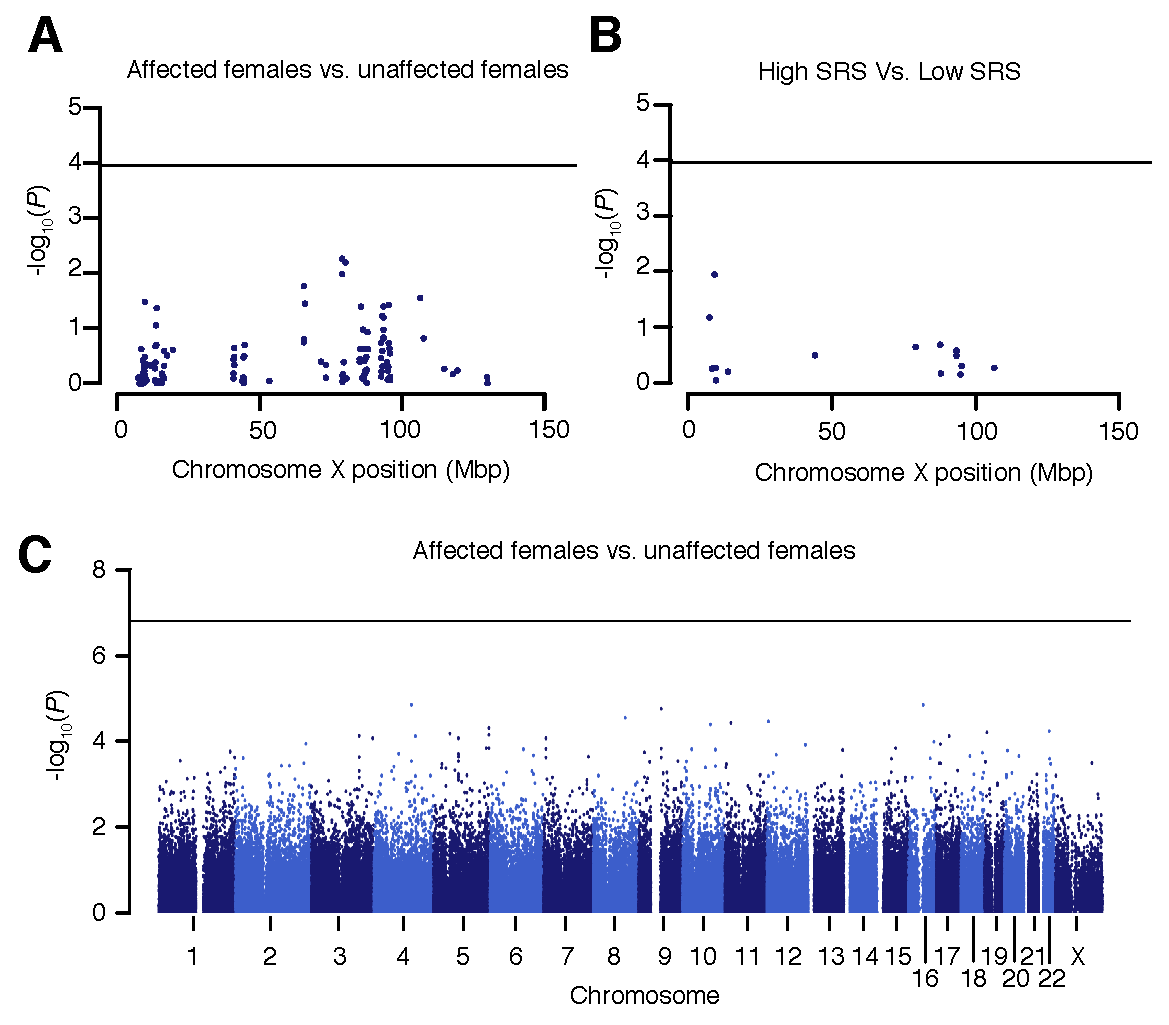
\includegraphics[width=\linewidth]{Sup_4_AGRE_Dom.pdf}
			\includegraphics[width=\linewidth]{Figures/ONE.png}
		\end{center}
		\caption{\textbf{Manhattan Plot of Association Results Under a Dominant Model in the AGRE Cohort. }}
		\label{Figure8}
		\textbf{A)} Loci on the X-Chromosome within regions shown to escape X-inactivation were examined between cases and controls in AGRE. The association test results under a dominant model are shown. \textbf{B)} The analysis was repeated using an SRS cut off value of 45 was used to distinguish cases (high SRS) from controls (low SRS), instead of ASD diagnostic status.  \textbf{C)} Using ASD diagnosis to identify cases and controls a genome-wide association analysis with a dominant model was performed. 
	\end{figure}
	\clearpage
}\normalsize

\afterpage{
	\begin{figure}[h!]
		\begin{center}
			%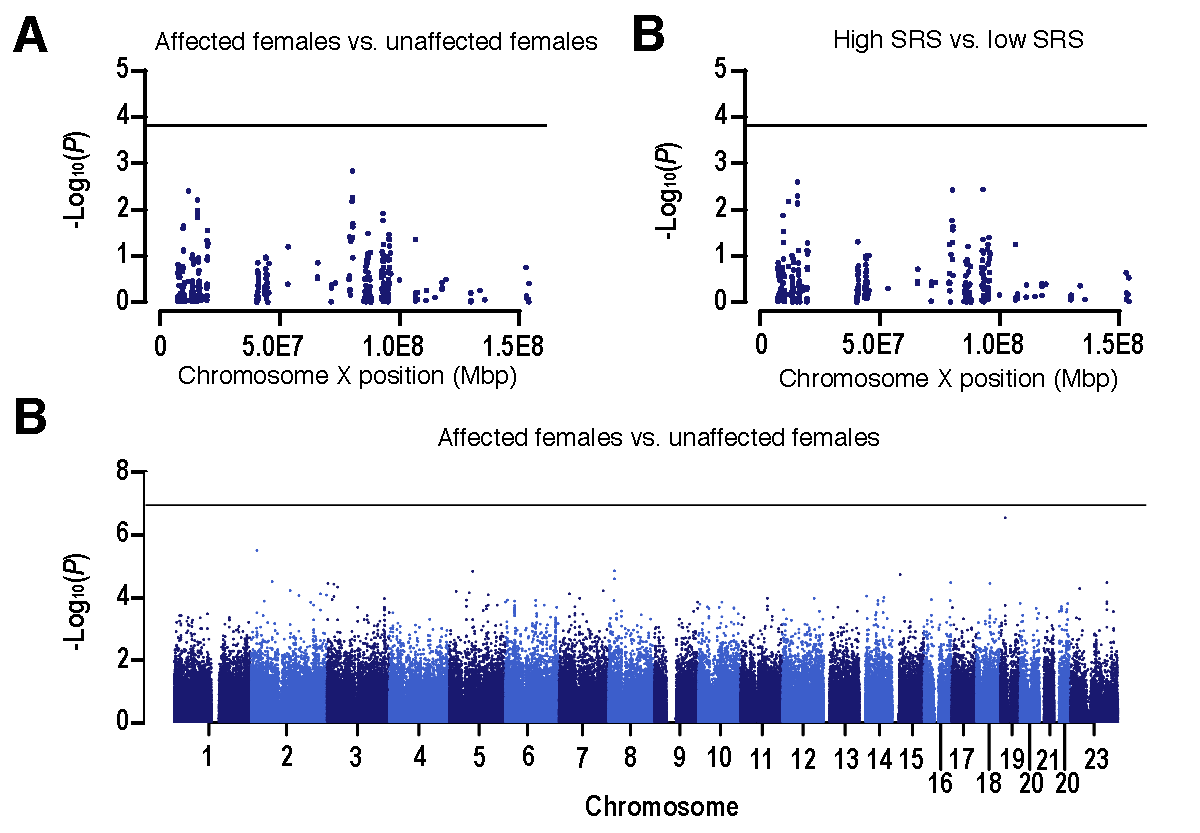
\includegraphics[width=\linewidth]{Sup_5_SSC_DomRast.pdf}
			\includegraphics[width=\linewidth]{Figures/TWO.png}
		\end{center}

		\caption{\textbf{Manhattan Plot of Association Results Under a Dominant Model in the SSC Cohort. }}
		\label{Figure9}
		\textbf{A)} Loci on the X-Chromosome within regions shown to escape X-inactivation were examined between cases and controls in SCC. The association test results under a dominant model are shown. \textbf{B)} The analysis was repeated using an SRS cut off value of 45 was used to distinguish cases (high SRS) from controls (low SRS), instead of ASD diagnostic status.  \textbf{C)} Using ASD diagnosis to identify cases and controls a genome-wide association analysis with a dominant model was performed. 
	\end{figure}
	\clearpage
}\normalsize

%%Recessive Model
\afterpage{
	\begin{figure}[h!]
		\begin{center}
			%\includegraphics[width=\linewidth]{Sup_6_AGRE_Rec.pdf}
			\includegraphics[width=\linewidth]{Figures/THREE.png}
		\end{center}
		\caption{\textbf{Manhattan Plot of Association Results Under a Recessive Model in the AGRE Cohort. }}
		\label{Figure10}
		\textbf{A)} Loci on the X-Chromosome within regions shown to escape X-inactivation were examined between cases and controls in AGRE. The association test results under a recessive model are shown. \textbf{B)} The analysis was repeated using an SRS cut off value of 45 was used to distinguish cases (high SRS) from controls (low SRS), instead of ASD diagnostic status.  \textbf{C)} Using ASD diagnosis to identify cases and controls a genome-wide association analysis with a recessive model was performed. 
	\end{figure}
	\clearpage
}\normalsize

\afterpage{
	\begin{figure}[h!]
	\begin{center}
			%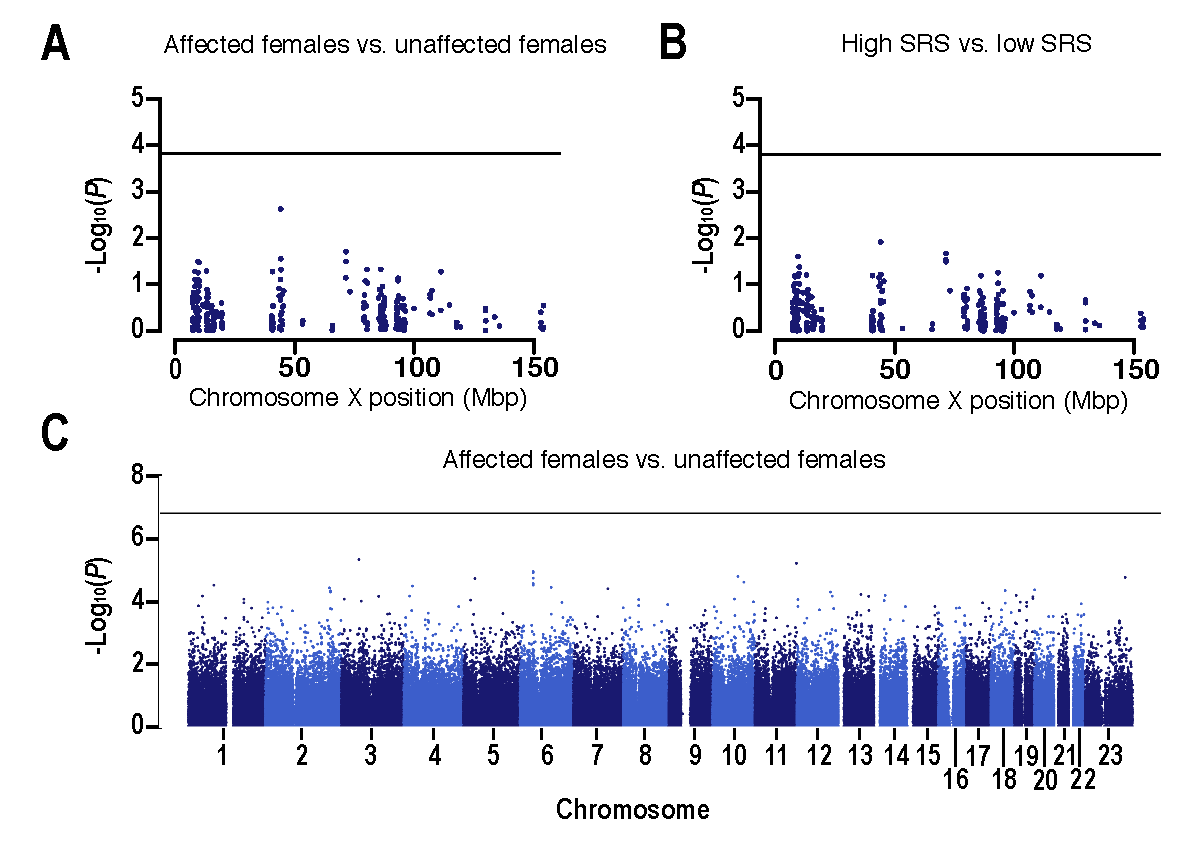
\includegraphics[width=\linewidth]{Sup_7_SSC_RecRast.pdf}
			\includegraphics[width=\linewidth]{Figures/FOUR.png}
		\end{center}
		\caption{\textbf{Manhattan Plot of Association Results Under a Recessive Model in the SSC Cohort. }}
		\label{Figure11}
		\textbf{A)} Loci on the X-Chromosome within regions shown to escape X-inactivation were examined between cases and controls in SSC. The association test results under a recessive model are shown. \textbf{B)} The analysis was repeated using an SRS cut off value of 45 was used to distinguish cases (high SRS) from controls (low SRS), instead of ASD diagnostic status. \textbf{C)} Using ASD diagnosis to identify cases and controls a genome-wide association analysis with a recessive model was performed. 
	\end{figure}
	\clearpage
}\normalsize

%%Additive Model
\afterpage{
	\begin{figure}[h!]
		\begin{center}
			%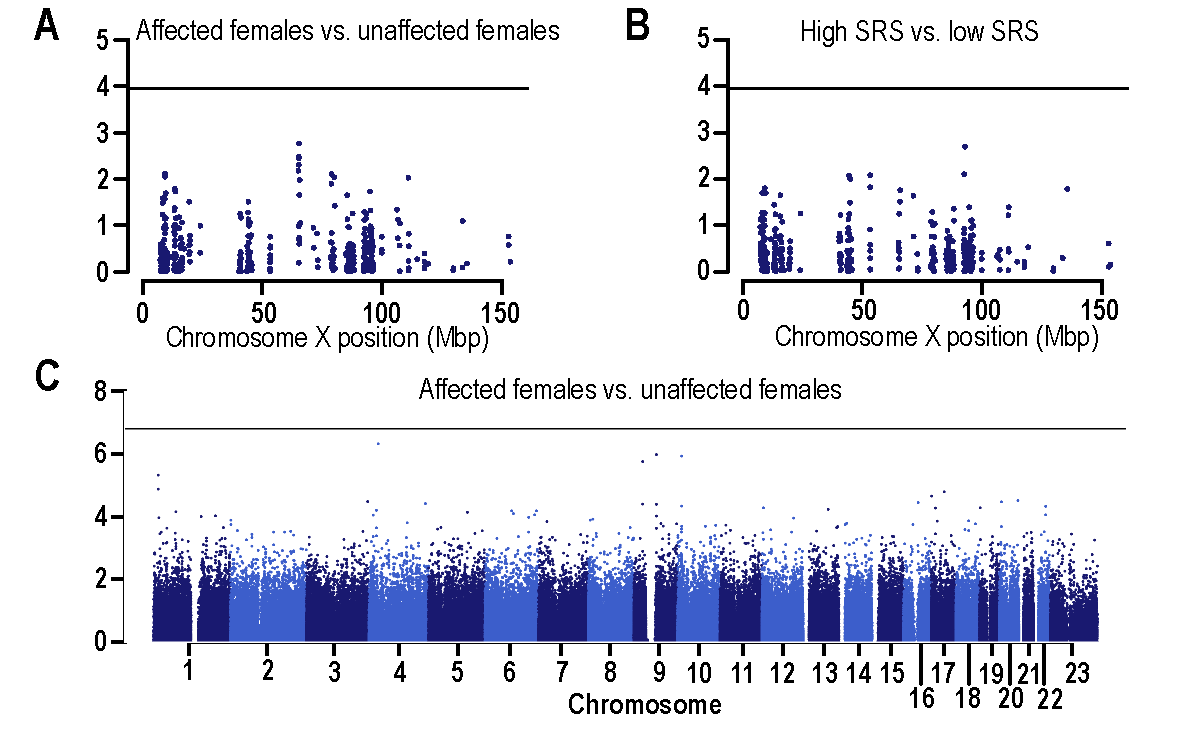
\includegraphics[width=\linewidth]{AGRE_Default_Rast.pdf}
			\includegraphics[width=\linewidth]{Figures/FIVE.png}
		\end{center}
		\caption{\textbf{Manhattan Plot of Association Results Under an Additive Model in the AGRE Cohort. }}
		\label{Figure12}
		\textbf{A)} Loci on the X-Chromosome within regions shown to escape X-inactivation were examined between cases and controls in SSC. The association test results under a recessive model are shown. \textbf{B)} The analysis was repeated using an SRS cut off value of 45 was used to distinguish cases (high SRS) from controls (low SRS), instead of ASD diagnostic status. \textbf{C)} Using ASD diagnosis to identify cases and controls a genome-wide association analysis with a recessive model was performed. 
	\end{figure}
	\clearpage
}\normalsize

\afterpage{
	\begin{figure}[h!]
		\begin{center}
			%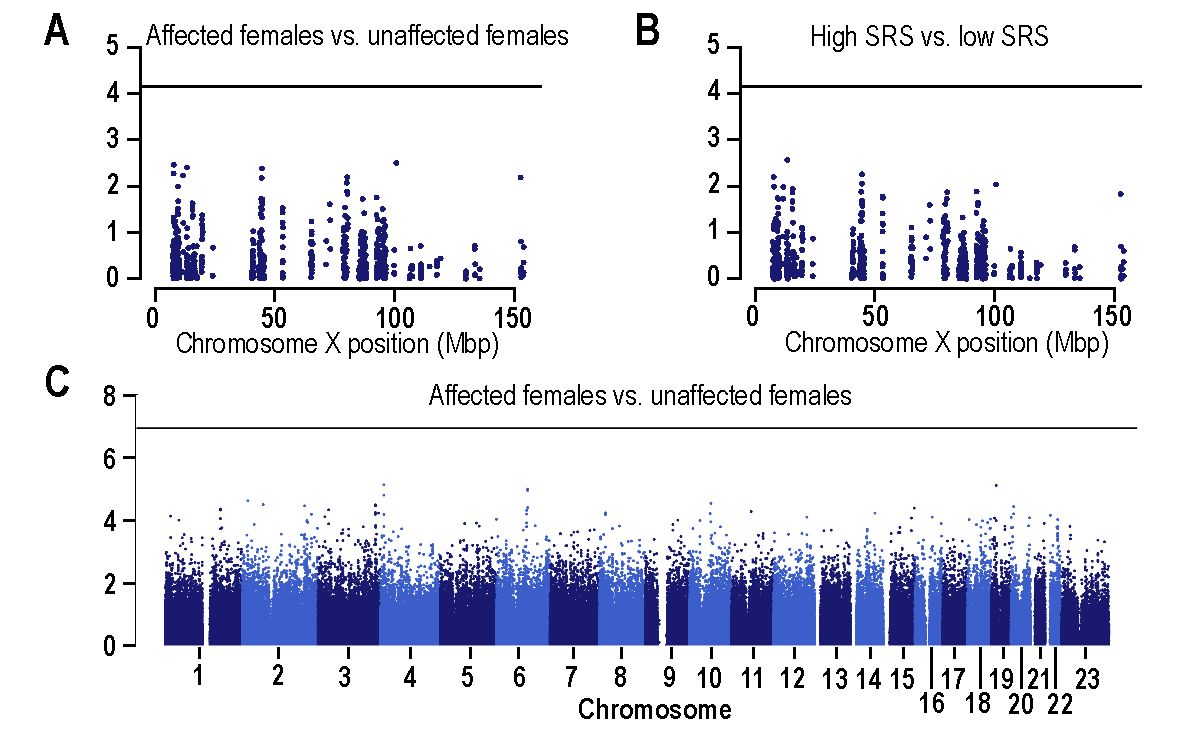
\includegraphics[width=\linewidth]{SSC_Default_Rast.pdf}
			\includegraphics[width=\linewidth]{Figures/SIX.png}
		\end{center}
		\caption{\textbf{Manhattan Plot of Association Results Under an Additive Model in the SSC Cohort. }}
		\label{Figure13}
		\textbf{A)} Loci on the X-Chromosome within regions shown to escape X-inactivation were examined between cases and controls in SSC. The association test results under a recessive model are shown. \textbf{B)} The analysis was repeated using an SRS cut off value of 45 was used to distinguish cases (high SRS) from controls (low SRS), instead of ASD diagnostic status. \textbf{C)} Using ASD diagnosis to identify cases and controls a genome-wide association analysis with a recessive model was performed. 
	\end{figure}
	\clearpage
}\normalsize

%%Alternate Anaylsis SNP table
\afterpage{
	\renewcommand{\arraystretch}{0.3}%
	\begin{table}[h!]
		\begin{center}
			\begin{tabular}{cccccc}

				Comparison&SNP&Chr&Position&P-Val&BF-Corrected\\		
				\hline													
				\\            

				 &rs7891218 & X & 92838948 & 2.0E-03 & 0.91 \\ 
				High SRS & rs5983514 & X & 92560942 & 7.9E-03 & 1 \\ 
				Versus & rs1409117 & X & 53319220 & 8.4E-03 & 1 \\ 
				Low SRS & rs2146335 & X & 44389803 & 8.6E-03 & 1 \\ 
				 & rs7050908 & X & 44918083 & 1.0E-02 & 1 \\ 

				\hline													
				\\

				 & rs6524008 & X & 107483616 & 4.4E-03 & 1 \\
				Affected, high SRS & rs6622146 & X & 106209321 & 4.6E-03 & 1 \\
				Versus & rs12014086 & X & 44065595 & 6.9E-03 & 1 \\
				Affected, low SRS & rs5990206 & X & 95558656 & 9.6E-03 & 1 \\
				 & rs10521610 & X & 10124322 & 1.0E-02 & 1 \\
				\hline													
				\\	

				 & rs12012307 & X & 19803729 & 3.4E-03 & 1 \\
				Affected, high SRS & rs4350137 & X & 93943526 & 4.2E-03 & 1 \\
				Versus & rs727090 & X & 13469667 & 4.6E-03 & 1 \\
				Unaffected, high SRS & rs1017874 & X & 19779567 & 5.7E-03 & 1 \\
				 & rs2285405 & X & 119262477 & 8.7E-03 & 1 \\
				\hline													
				\\	

				 & rs881599 & X & 9135603 & 2.7E-03 & 1 \\
				Affected, high SRS & rs2317959 & X & 94641848 & 3.9E-03 & 1 \\
				Versus & rs2074098 & X & 13735538 & 5.3E-03 & 1 \\
				Unaffected, low SRS & rs5978769 & X & 7808157 & 1.5E-02 & 1 \\
				 & rs12688370 & X & 13806166 & 1.6E-02 & 1 \\
				\hline													
				\\	

				 & rs5935671 & X & 13786582 & 2.0E-03 & 0.89 \\
				Affected, low SRS & rs5990206 & X & 95558656 & 2.9E-03 & 1 \\
				Versus & rs5936079 & X & 15867223 & 3.7E-03 & 1 \\
				Unaffected, high SRS & rs234495 & X & 15348936 & 7.1E-03 & 1 \\
				 & rs11796661 & X & 86749681 & 8.7E-03 & 1 \\
				\hline													
				\\	

				 & rs6622146 & X & 106209321 & 3.1E-03 & 1 \\
				Affected, low SRS & rs5949895 & X & 95725873 & 5.6E-03 & 1 \\
				Versus & rs1983481 & X & 8292613 & 7.0E-03 & 1 \\
				Unaffected, low SRS & rs5990153 & X	& 95028102 & 1.3E-02 & 1 \\
				 & rs12688370 & X & 13806166 & 1.3E-02 & 1 \\
				\hline													
				\\	

				& rs5949895 & X & 95725873 & 5.6E-04 & 0.25 \\
				Unaffected, high SRS & rs234495 & X & 15348936 & 2.9E-03 & 1 \\
				Versus & rs5936079 & X & 15867223 & 1.0E-02 & 1 \\
				Unaffected, low SRS & rs5913240 & X & 79384683 & 1.0E-02 & 1 \\
				& rs12834592 & X & 92669150 & 1.2E-02 & 1 \\
				\hline													
				\\	
				\end{tabular}
			\caption{\textbf{AGRE Association Test Results Based on SRS Defined Case/Control Definitions }}
			\label{Table4}
		\end{center}
		Considering the possibility that the protective status of the females may not correlate well with ASD diagnosis, we compared females in AGRE based on a combination of SRS and ASD categorical diagnosis (Figure \ref{fig:agresrs}). The top five SNPs in each analysis are shown.
	\end{table}
	\clearpage
}\normalsize

%%AGRE Stratification
\afterpage{
	\begin{figure}[h!]
		\begin{center}
			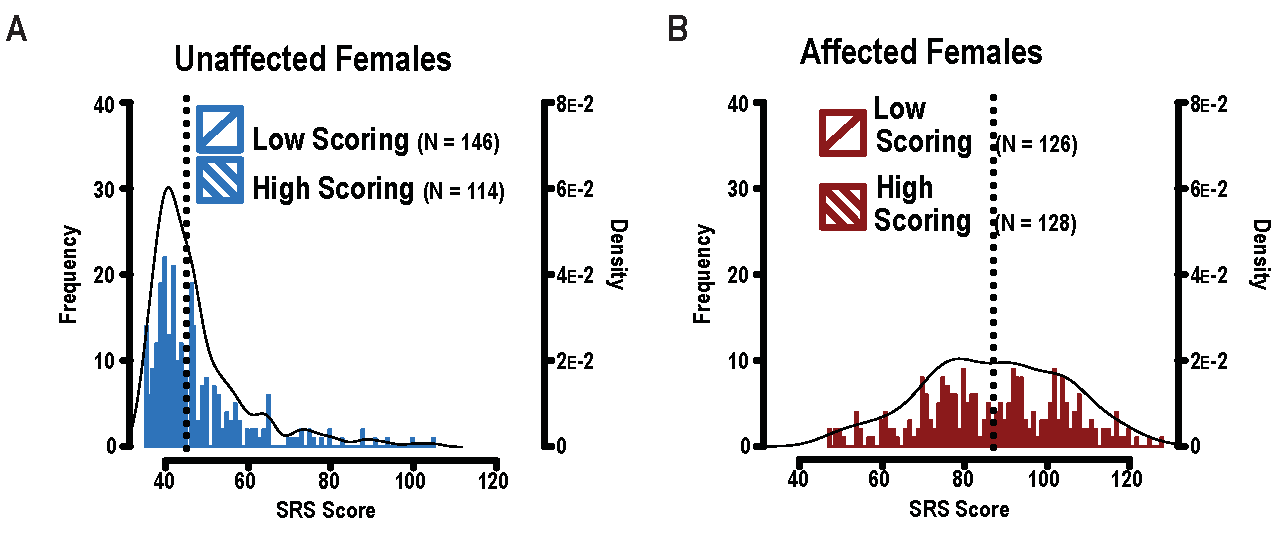
\includegraphics[width=\linewidth, height=6.5in, keepaspectratio=TRUE]{Figures/Sup_8.pdf}
		\end{center}
		\caption{\textbf{Stratification of AGRE Affected and Unaffected Females by SRS Score.}}
		\label{Figure14}
		\textbf{A)} Unaffected females were stratified into a higher scoring (N=114) and lower scoring (N=146) population based on an SRS score of 45. After data cleaning, and considering only unrelated samples of European ancestry, the samples sizes were 54 and 64 respectively. \textbf{B)} Affected females were stratified at the 50th percentile into higher scoring (N=128) and lower scoring (N=126) groups. After data cleaning, and considering only unrelated samples of European ancestry, the samples sizes were 58 and 51 respectively.
	\end{figure}
	\clearpage
}\normalsize


%%Ascertainment Bias
\afterpage{
	\begin{figure}[h!]
		\begin{center}
			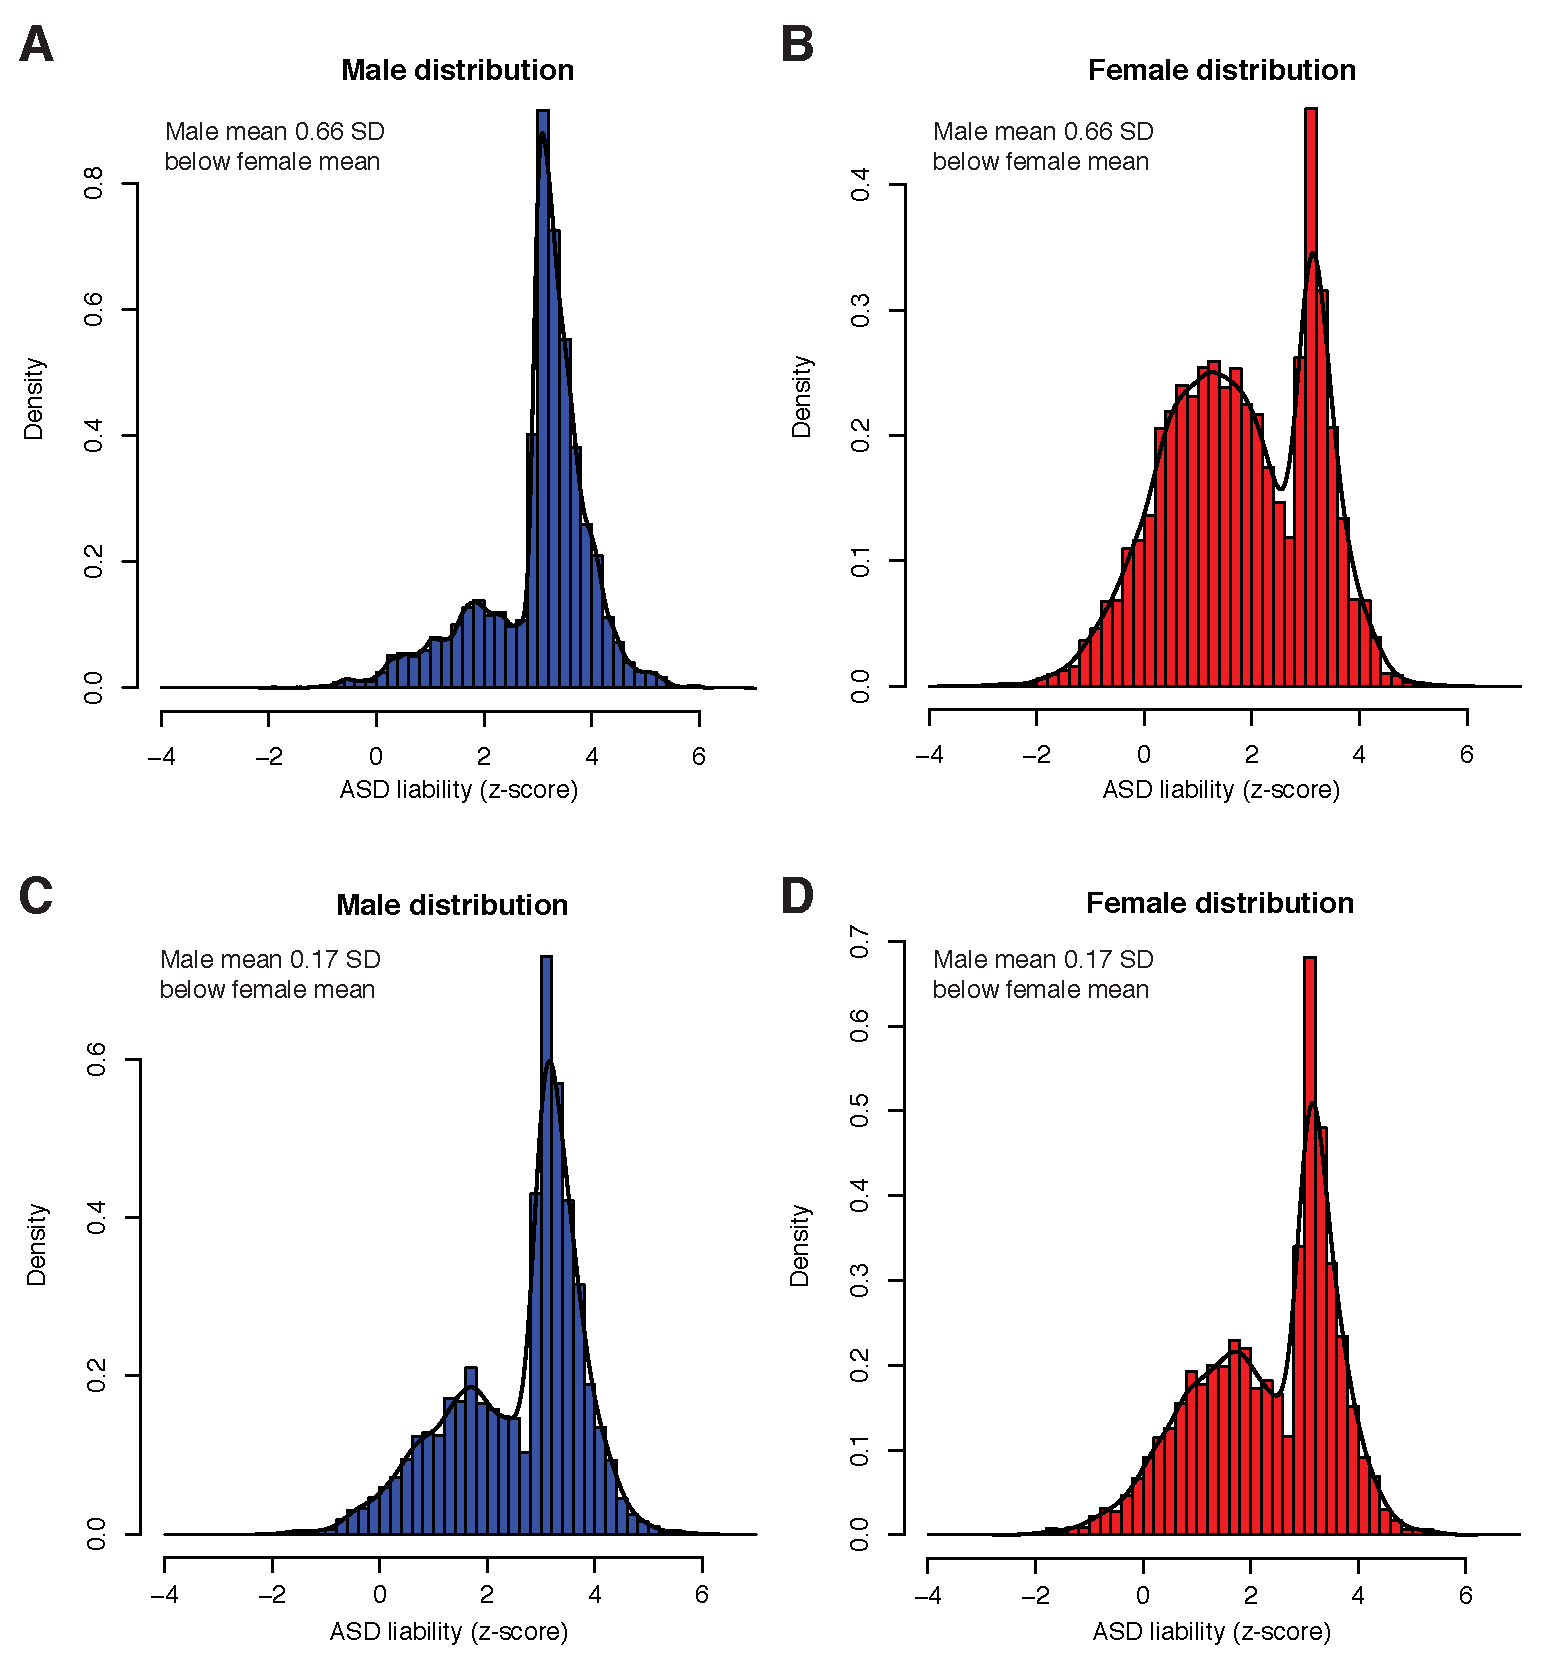
\includegraphics[width=.8\linewidth]{AscertainmentBias.pdf}
		\end{center}
		\caption{\textbf{Effect of Ascertainment Bias on ASD Liability}}
		\label{Figure15}
 		\textbf{A)} Distribution of ASD liability in males in simulated families selected using the ascertainment methods used in the AGRE collection (at least two affected children). The male and female mean liability was shifted by 0.66 standard deviations to give a 4:1 sex bias and the diagnostic threshold was selected to give an incidence of 1\%. \textbf{B)} The female liability distribution under the same model as `A'. \textbf{C)} The simulation was repeated using a shift of 0.17 standard deviations which is equivalent to the difference of 3 SRS points observed between male and female samples. \textbf{D)} The female liability distribution under the same model as `C'.
	\end{figure}
	\clearpage
}\normalsize

\section{Results}
	\subsection{Targeted Association Study: Tier 1 SNPs}
		To test the hypothesis that the FPE is mediated by a common variant at a single locus an association test comparing 208 affected females against 151 unrelated unaffected females was performed. Since the FPE is unique to females, it was reasoned that the region of the genome that has the greatest potential for sexual dimorphism would be the most likely location for such a locus, therefore the first tier of the analysis was performed on 451 SNPs that are unique to chromosome X and that escape X-inactivation (Figure \ref{Figure5} and Table \ref{Table1A}). No SNPs were significant after correcting for the 451 comparisons (Figure \ref{Figure16}). Of the top five SNPs (Table \ref{Table5}), only three had a dominant risk allele that was observed more frequently in the affected females (odds ratio $>$ 1) and none had allele frequencies close to the prediction in both the affected and unaffected groups. Only one of these five SNPs was represented on the microarrays used for the SSC replication cohort (207 affected females, 676 unaffected females); despite this SNP reaching nominal significance, the dominant risk allele was more frequent in the unaffected group, i.e. the opposite direction of effect observed in the discovery sample. Given the targeted nature of this analysis, the estimated power to discover a single locus meeting the hypothesis was 100\% even with modest enrichment of unprotected females in the affected group (Figure \ref{Figure2}).

	\subsection{Targeted Association Study: Tier 2 SNPs}
    
    	Since no clear candidates were observed in the tier 1 SNPs, the analysis was expanded to the whole of chromosome X to account for the possibility that that of regions escaping X-inactivation may not be complete. As with the tier 1 analysis, no SNPs showed significant association after correcting for the 6,955 comparisons (Figure \ref{Figure16}B). Considering the top SNPs (Table \ref{Table6}), all five showed a direction of effect that was the opposite of expectation given the allele frequencies (see Supplemental Methods). None of these SNPs were nominally significant in the SSC replication cohort. Of note, none of the top five SNPs from the tier 1 analysis were in the top five for the tier 2 analysis, despite all 451 tier 1 SNPs being included in this analysis. The statistical power to detect the hypothesized single FPE locus was still estimated to be 100\% for tier 2.
        
     \subsection{Genome Association Study: Tier 3 SNPs}
			
        Next, the possibility that the protective allele was not on chromosome X, (e.g. an autosomal gene that was only expressed in the presence of high estrogen levels) was considered. Therefore the analysis was repeated for all 317,574 SNPs in the AGRE group. Again there was no association after correction for multiple comparisons (Figure \ref{Figure16}C) and none of the top five SNPs were nominally significant in the replication group (Table \ref{Table7}). Of note, none of the top five SNPs were on chromosome X. Even with the larger number of SNPs, we estimated our power to detect the hypothesized single FPE locus to be 100\% (Figure \ref{Figure4}).
            
    \subsection{Exploratory Association Analyses}        
      	
        Finally, the possibility that our inability to detect the hypothesized single FPE locus was due to inaccurate differentiation of females with, and without, the FPE was considered . For instance, a female may be unaffected due to the absence of risk factors despite absent FPE. Therefore cases and controls were defined by their SRS score rather than by categorical ASD diagnoses. No SNPs were significant after multiple comparisons (Figures \ref{Figure8},\ref{Figure9},\ref{Figure10},\ref{Figure11}, and Table \ref{Table4}). Next, whether extremes of the affected and unaffected SRS distributions might be enriched for females in whom the FPE was present or absent was considered (Figure \ref{Figure14}). Again, no SNPs were significant after multiple comparisons (Table \ref{Table4}). In addition, all of the reported analyses were preformed under an additive model; no genome-wide significant SNPs were identified (Figure \ref{Figure12} and \ref{Figure13}, Table \ref{Table8} and \ref{Table9}).                 
            
            
\afterpage{
    \begin{figure}[h!]
		\centering
		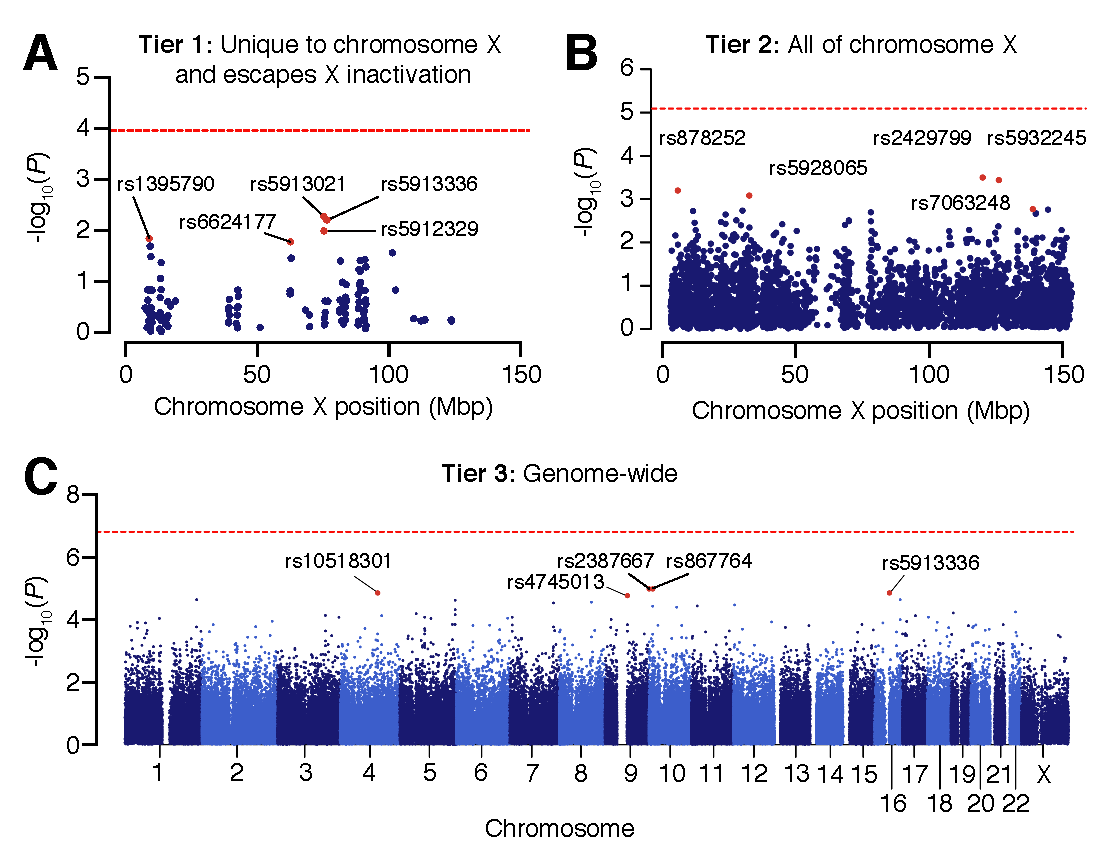
\includegraphics[width=1\textwidth]{Figures/Figure_4_GWAS_Gockley_Dec2014.pdf}
        		\caption{\textbf{Manhattan Plots of Association Study Results.}  \label{Figure16}}     	
       		\begin{flushleft}Results of association studies comparing 208 affected females and 151 unaffected females from AGRE. To maximize the ability to identify a candidate variant for the FPE the association test was performed on three tiers of SNPs, based on the a priori probability of mediating the FPE. A) Tier 1: 451 SNPs unique to chromosome X that escape X inactivation. No SNPs are significant after multiple comparisons (horizontal red line). The top five SNPs (red) are labeled (Table \ref{Table1}). B) Tier 2: all 6,955 SNPs on chromosome X. No SNPs are significant after multiple comparisons (horizontal red line). The top five SNPs (red) are labeled (Table \ref{Table2}). C) Tier 3: all 317,574 SNPs across the genome. No SNPs are significant after multiple comparisons (horizontal red line). The top five SNPs (red) are labeled (Table \ref{Table3}). 
       		\end{flushleft}
	\end{figure}
	\clearpage
	}
    \normalsize

\afterpage{
	\scriptsize 
    \begin{table}[h!]
		\renewcommand{\arraystretch}{.6}
        \centering
        	\resizebox{1.0\textwidth}{!}{%
			\begin{tabular}{ccccccccccc}
					 
				 & \multicolumn{6}{c}{\underline{AGRE Discovery (208 cases, 151 Controls)}} & \multicolumn{4}{c}{\underline{SSC Repplication (207 cases, 676 Controls)}} \\ 
 
\textbf{SNP} 	& Allele 1/ & Aff Allele  & UnAff Allele & Odds  &   P    & Corr P   & Aff Allele  & UnAff Allele & Odds  & P       \\ 
				& Allele 2 & 1 Freq (\%) & 1 Freq (\%)  & Ratio  & Value  & P-Value   & 1 Freq (\%) & 1 Freq (\%)  & Ratio & Value   \\ \hline
Predicted		&          &    97.0     &   $<$24.3    &   $>$88& $\leq1*10^{-8}$&  $\leq0.05$   & 97.0      &  $<$24.3     &$>$88  & $\leq1*10^{-8}$ \\ 
rs5913021 		&  G/A     &    71.5     &     57.3     &   1.25 & 0.005  &  1.0  &               &           &       &         \\ 
rs5913336 		&  A/G     &    49.0     &     63.6     &   0.77 & 0.006  &  1.0  &       69.9    & 60.9      &  1.14 &  0.007  \\ 
rs5912329 		&  A/G     &    71.4     &     58.2     &   1.23 &  0.01  &  1.0  &               &           &       &         \\ 
rs1395790 		&  G/A     &     2.4     &      7.9     &   0.30 &  0.01  &  1.0  &               &           &       &         \\ 
rs6624177 		&  A/G     &    60.0     &     72.2     &   0.83 &  0.02  &  1.0  &               &           &       &         \\ 
			\end{tabular}%
            }
			\caption{\textbf{Top Five SNPs from Tier 1 Analysis}}
			\label{Table5}
	\end{table}
	\clearpage
}\normalsize

\afterpage{
	\scriptsize 
    \begin{table}[h!]
		\renewcommand{\arraystretch}{.6}
        \centering
        	\resizebox{1.0\textwidth}{!}{%
			\begin{tabular}{ccccccccccc}
					 
				 & \multicolumn{6}{c}{\underline{AGRE Discovery (208 cases, 151 Controls)}} & \multicolumn{4}{c}{\underline{SSC Repplication (207 cases, 676 Controls)}} \\ 
 
\textbf{SNP} 	& Allele 1/ & Aff Allele  & UnAff Allele & Odds   & P      & Corr P   & Aff Allele  & UnAff Allele & Odds  & P       \\ 
				& Allele 2 & 1 Freq (\%) & 1 Freq (\%)  & Ratio  & Value  & P-Value  & 1 Freq (\%) & 1 Freq (\%)  & Ratio & Value   \\ \hline
Predicted		&          &    97.0     &   $<$24.3    &   $>$88& $\leq1*10^{-8}$&  $\leq0.05$   & 97.0      &  $<$24.3     &$>$88  & $\leq1*10^{-8}$ \\ 
rs2429799&  A/G     &    21.2     &      7.3     &   2.90 & 0.0003 & 1.0   &               &           &       &         \\ 
rs5932245&  A/G     &    97.1     &     87.4     &   1.11 & 0.0004 & 1.0   &     54.1      &   55.0    &  0.98 & 0.9645   \\ 
rs878252 &  G/A     &    31.7     &     15.9     &   2.00 & 0.0006 & 1.0   &     29.0      &   25.6    &  1.13 & 0.1699  \\ 
rs5928065&  G/A     &    94.7     &     84.1     &   1.13 & 0.0008 & 1.0   &     88.4      &   93.3    &  0.95 & 0.5674  \\ 
rs7063248&  G/A     &    73.4     &     57.6     &   1.27 & 0.0017 & 1.0   &     97.1      &   96.6    &  1.01 & 0.1885  \\ 									\end{tabular}%
            }
			\caption{\textbf{Top Five SNPs from Tier 2 Analysis}}
			\label{Table6}
	\end{table}
	\clearpage
}\normalsize

\afterpage{
	\scriptsize 
    \begin{table}[h!]
		\renewcommand{\arraystretch}{.6}
        \centering
        	\resizebox{1.0\textwidth}{!}{%
			\begin{tabular}{ccccccccccc}
					 
				 & \multicolumn{6}{c}{\underline{AGRE Discovery (208 cases, 151 Controls)}} & \multicolumn{4}{c}{\underline{SSC Repplication (207 cases, 676 Controls)}} \\ 
 
\textbf{SNP} 	& Allele 1/ & Aff Allele  & UnAff Allele & Odds   & P      & Corr P   & Aff Allele  & UnAff Allele & Odds  & P       \\ 
				& Allele 2 & 1 Freq (\%) & 1 Freq (\%)  & Ratio  & Value  & P-Value  & 1 Freq (\%) & 1 Freq (\%)  & Ratio & Value   \\ \hline
Predicted		&          &    97.0     &   $<$24.3    &   $>$88& $\leq1*10^{-8}$&  $\leq0.05$   & 97.0      &  $<$24.3     &$>$88  & $\leq1*10^{-8}$ \\ 
rs2387667 &  G/A     &    33.7     &     13.2     &   2.54 & $1.1*10^{-5}$ &  1.0  &    15.9       &   19.5    &  0.82 & 0.25    \\ 
rs867764  &  A/G     &    33.7     &     13.2     &   2.54 & $1.1*10^{-5}$ &  1.0  &    23.2       &   23.5    &  0.99 & 0.92    \\ 
rs10518301&  A/G     &    25.0     &     47.0     &   0.53 & $1.4*10^{-5}$ &  1.0  &    40.1       &   41.1    &  0.98 & 0.79    \\ 
rs9302760 &  A/G     &    75.0     &     53.0     &   1.42 & $1.4*10^{-5}$ &  1.0  &    60.4       &   56.4    &  1.07 & 0.31    \\ 
rs4745013 &  G/A     &    36.1     &     58.9     &   0.61 & $1.7*10^{-5}$ &  1.0  &    49.8       &   47.8    &  1.04 & 0.62    \\ 
			\end{tabular}%
            }
			\caption{\textbf{Top Five SNPs from Tier 3 Analysis}}
			\label{Table7}
	\end{table}
	\clearpage
}\normalsize

%%Additive Model SNP table - AGRE
\afterpage{
	\renewcommand{\arraystretch}{0.3}%
	\begin{table}[h!]
		\begin{center}
			\begin{tabular}{cccccc}

				Comparison&SNP&Chr&Position&P-Val&BF-Corrected\\		
				\hline													
				\\

				%%Afected vs Unaffected
				& rs1028348 & X & 65384163 & 1.7E-03 & 0.77 \\
				Affected & rs670546 & X & 65272116 & 3.3E-03 & 1 \\
				Versus & rs5965083 & X & 65230426 & 3.6E-03 & 1 \\
				Unaffected & rs5964488 & X & 65253769 & 4.9E-03 & 1 \\
				& rs6525038 & X & 65193018 & 6.7E-03 & 1 \\
				\hline													
				\\

				%%High low SRS
				& rs7891218 & X & 92952292 & 2.0E-03 & 0.91 \\
				High SRS & rs5983514 & X & 92674286 & 7.9E-03 & 1 \\
				Versus & rs1409117 & X & 53302495 & 8.4E-03 & 1 \\
				Low SRS & rs2146335 & X & 44504859 & 8.6E-03 & 1 \\
				 & rs7050908 & X & 45033139 & 1.0E-04 & 1 \\
				\hline													
				\\	

				%%GWAS
				& rs7668302 & 4 & 29852055 & 4.8E-07 & 0.15 \\
				& rs4745013 & 9 & 72277423 & 1.1E-06 & 0.34 \\
				GWAS & rs867764 & 10 & 12794868 & 1.2E-06 & 0.38 \\
				& rs7020846 & 9 & 28393443 & 1.8E-06 & 0.56 \\
				& rs9943244 & 1 & 15268468 & 4.8E-06 & 1 \\
				\hline													
				\\	

			\end{tabular}
			\caption{\textbf{Top SNPs from Additive Model Analysis of the AGRE Cohort}}
			\label{Table8}
		\end{center}
	\end{table}
	\clearpage
}\normalsize

%%Additive Model SNP table - SSC
\afterpage{
	\renewcommand{\arraystretch}{0.3}%
	\begin{table}[h!]
		\begin{center}
			\begin{tabular}{cccccc}

				Comparison&SNP&Chr&Position&P-Val&BF-Corrected\\		
				\hline													
				\\

				%%Afected vs Unaffected
				& rs6621080 & X & 100630202 & 3.2E-03 & 1 \\
				Affected & rs845127 & X & 7785325 & 3.4E-03 & 1 \\
				Versus & rs5979883 & X & 13390855 & 4.0E-03 & 1 \\
				Unaffected & rs7058967 & X & 44592534 & 4.1E-03 & 1 \\
				& rs16984793 & X & 7815994 & 5.3E-03 & 1 \\
				\hline													
				\\

				%%High low SRS

				& rs5979883 & X & 13390855 & 2.7E-03 & 0.91 \\
				High SRS & rs7058967 & X & 44592534 & 5.5E-03 & 1 \\
				Versus & rs845127 & X & 7785325 & 6.3E-03 & 1 \\
				Low SRS & rs12846943 & X & 44607553 & 8.9E-03 & 1 \\
				& rs6621080 & X & 100630202 & 9.2E-03 & 1 \\
				\hline													
				\\	

				%%GWAS
				& rs1454870 & 4 & 11884740 & 7.3E-06 & 1 \\
				& rs12462380 & 19 & 16298048 & 7.7E-06 & 1 \\
				GWAS & rs1054227 & 6 & 100097577 & 1.0E-05 & 1 \\
				& rs2296154 & 6 & 100099989 & 1.1E-05 & 1 \\
				& rs2124141 & 4 & 11851124 & 1.6E-06 & 1 \\
				\hline													
				\\	

				\end{tabular}
			\caption{\textbf{Top SNPs from Additive Model Analysis of the SSC Cohort}}
			\label{Table9}
		\end{center}
	\end{table}
	\clearpage
}\normalsize

	\section{Discussion}

	The observation of a bimodal SRS distribution in females, but not males, from multiplex families raised the possibility of a single genetic locus mediating a female protective effect and resulting in a 4:1 sex bias in ASD. Given the potential of such a locus as a therapeutic target, and the high likelihood that such a locus would be missed by a GWAS with mixed sexes, this association study, which was well powered to detect such an effect was preformed.
	\par Three tiers of SNPs were considered, these were based on the a priori probability that genomic regions might harbor a single locus for FPE. The first tier considered only SNPs unique to chromosome X that escaped X-inactivation, the second tier considered all SNPs on chromosome X, and the third tier was a full genome-wide association study. No SNPs reached significance after correcting for multiple comparisons in any of the three tiers (Figure \ref{Figure16}); furthermore there was no evidence of replication in the SSC cohort, nor of a SNP in one tier being present in the top five SNPs of the next tier. This result was unchanged by an additive model (Figure \ref{Figure12} and \ref{Figure13}), defining case/control status using the SRS score (Figures \ref{Figure14}, Table \ref{Table4}), or considering the extremes of the SRS distribution (\ref{Table4}). 
	\par The female-only GWAS achieved considerably higher power than a GWAS with both sexes and was extremely well powered to detect a single locus for the FPE even with marked deviation from the expected allele frequency (Figure \ref{Figure4}). Therefore it can be concluded that the FPE is unlikely to be mediated by a single genetic locus. This negative result does not reduce the likelihood of a female protective effect being responsible for the sex bias observed in ASD, nor does it reduce the likelihood of this protection being mediated by a polygenic effect. 
	\par There are several explanations for this negative result. First, there may be little variance in the FPE between females. For example, if the FPE was mediated by endogenous estrogen levels above a certain threshold, and all females exceeded this threshold, then the FPE would be constant without genetic or environmental risk factors having an effect.Recent evidence after this work was published points to a potential mechanism of estrogen mediated rescue of potential ASD behavior in zebra fish\cite{Hoffman:2016aa}. Alternatively, the FPE may vary between females, but this variance is determined by multiple genetic and/or environmental factors, for example if the extent of FPE was dependent on the degree of endogenous estrogen exposure. Finally, it is possible that a single environmental factor (e.g. exogenous estrogen exposure) determines the presence of the FPE, though such a factor would need to act in the majority of females, but not act in the majority of males.
	\par The first explanation (FPE in all females) would not lead to the bimodal SRS distribution that prompted this study (Figure \ref{Figure1}H), while the second (multifactorial FPE) could only produce a bimodal distribution if the majority of risk factors targeted a common biological pathway or neurological process (Figure \ref{Figure1}F). It is hard to reconcile the third explanation (a single environmental effect) with the consistent sex bias observed across so many studies. 
	\par This leads towards considering alternative explanations for the bimodal distribution. Firstly there's the consideration of ‘non-biological’ biases in the manner of data collection. One possibility is ascertainment bias, i.e. that unaffected males are rare in multiplex families, while unaffected females are detected comparatively frequently. Simulation of multiplex families shows that ascertainment bias and a 4:1 sex bias can induce a bimodal distribution in ASD liability that is more pronounced in females (Figure \ref{Figure15}A and \ref{Figure15}B). However, this is most likely not the complete explanation of the SRS distribution since the observed data differs from the expectation of this model in two important respects: 	
	\par First, the lower distribution in females (Figure \ref{Figure15}B) has a mean over one standard deviation above the general population (equivalent to an SRS score of over 40). However, in the multiplex females (Figure \ref{Figure1}B) the lower distribution females is the same as the general population (SRS of 18). 
	\par Second, the simulation required a difference in mean liability between males and females of 0.66 standard deviations (equivalent to an SRS of 12). However, the observed SRS difference between males and females is four-fold lower at 0.17 standard deviations (equivalent to an SRS of 3). If the simulation is repeated using a sex difference of 0.17 standard deviations we observe little distinction between the male and female distributions (Figure \ref{Figure15}C and \ref{Figure15}D). 
	\par Therefore, while ascertainment bias may partially explain the bimodal SRS in multiplex females, these analyses suggest it is not the complete explanation of this phenomenon. Similarly, the effect may be a consequence of the sex of the parent rating the child for the SRS score. However, no such rater bias was detected in epidemiologic sample of twins\cite{Constantino:2003aa,Constantino:2005aa} and the bimodal distribution has been observed for SRS scored by both parents and teachers\cite{Virkud:2009aa}. Finally, it was considered whether IQ could confound the SRS score, however, only a very weak correlation between the two measures with a similar slope in males and females was observed(Figure \ref{Figure17}).
	\par Next ‘biological’ explanations for the bimodal distribution were considered. The ‘single locus’ observed may represent a rare risk factor rather than a rare protective factor, e.g. inherited large copy number variation (CNV). The distribution may also be a consequence of more complex interactions between multiple factors mediating protection and risk. For example, a general population twin study\cite{Constantino:2003aa} observed that reciprocal social behavior in females, but not males, was influenced by rearing factors that operated in the direction of promoting social competency. Further exploration of the manner in which inherited liability to ASD might capitalize upon, or accentuate, developmental sexual dimorphisms in gene expression, neuroanatomy, or behavior are warranted. It is of note that a large family study\cite{Constantino:2010aa} observed that a high proportion of the unaffected sisters of ASD probands manifested histories of early language delay with autistic qualities of speech which later resolved. These observations offer potential clues to the manner in which FPE might offset risk in the setting of autism susceptibility early in life.
	\par Microarray and exome sequencing studies have observed an excess \textit{de novo} mutation burden in ASD affected females compared to ASD affected males\cite{Dong:2014aa,Jacquemont:2014aa,Sanders:2011aa,Levy:2011aa}; however a quantitative relationship was not observed between CNV trait burden and ASD symptom severity. This underscores the possibility that FPE operates in a dichotomous manner, either offering complete protection from ASD risk or being completely overwhelmed by an excess of ASD risk.
	\par In summary, the distribution of ASD severity in females raised the possibility of an ASD protective effect in females mediated by a single genetic locus. If present, such a locus is likely to have been missed by prior GWAS analyses and would have great potential as a therapeutic target. However, this study represents a well-powered targeted association that found no evidence of such a genetic locus. The FPE remains of great interest as a route to discovering therapeutic targets, however the mechanism of this protection remains unknown. 

\afterpage{
	%%IQ vs. SRS
	\begin{figure}[h!]
		\begin{center}
			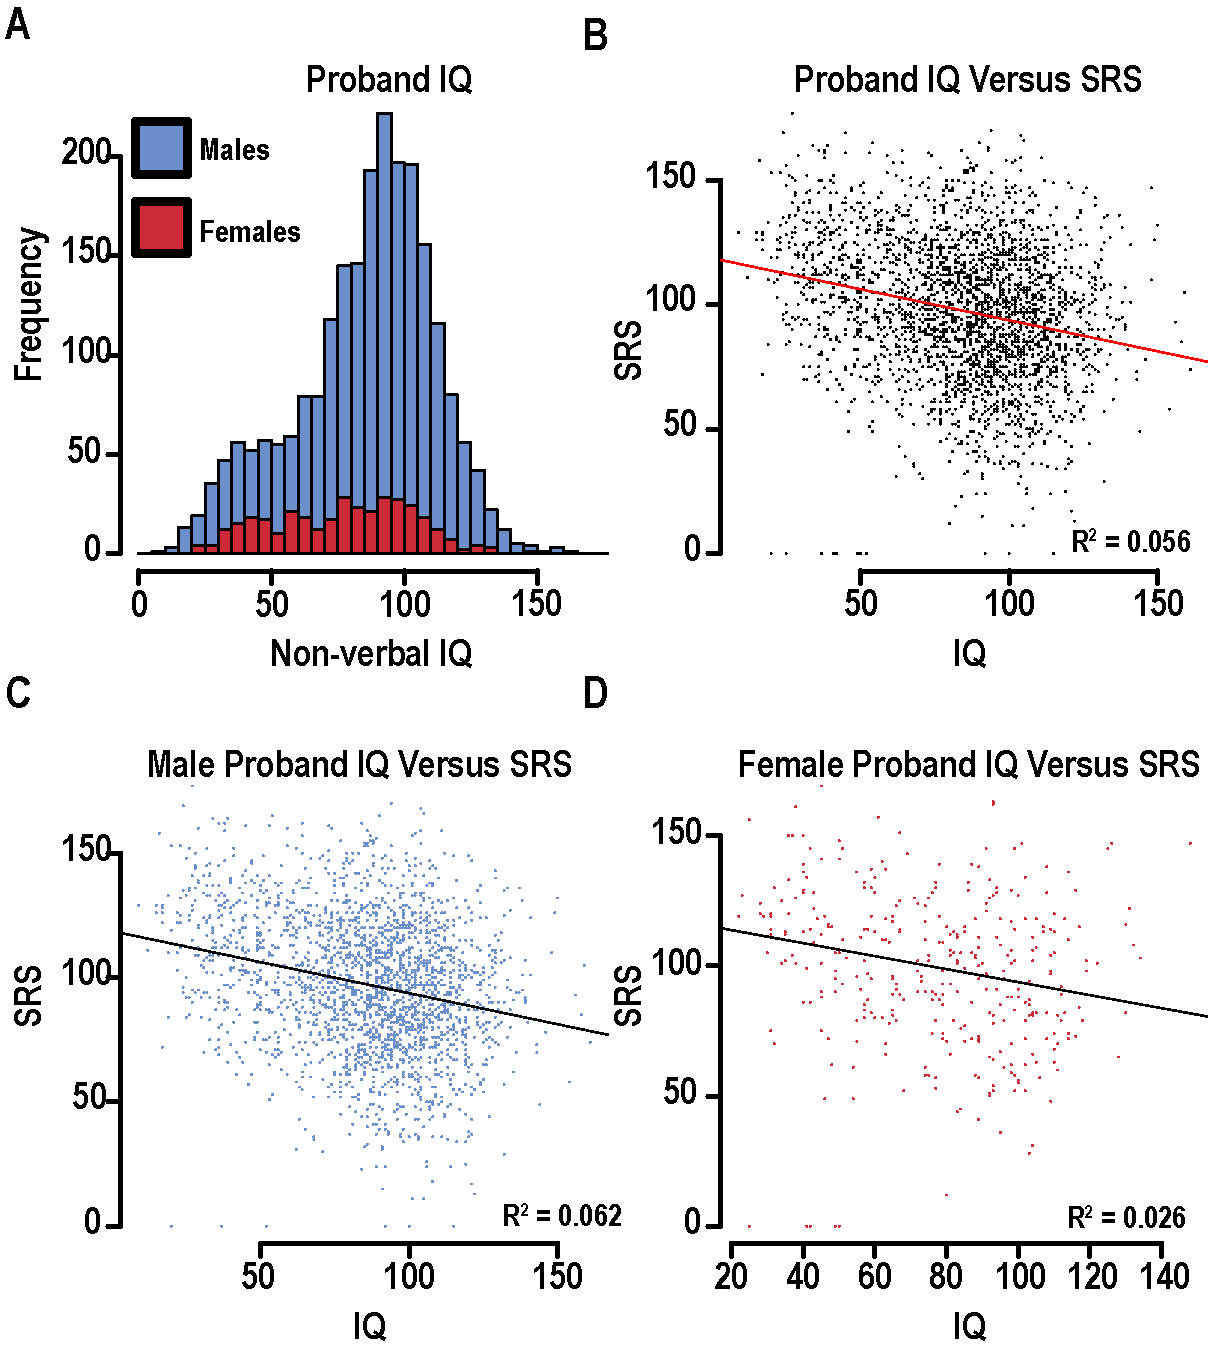
\includegraphics[width=.9\linewidth]{Figures/IQv2.pdf}
		\end{center}
		\caption{\textbf{IQ Distribution in SSC Probands}}
		\label{Figure17}
		\textbf{A)} Histogram of male (blue) and Female (red) IQ distributions in SSC probands.  \textbf{B)} Plot of SRS as a function of IQ in SSC probands. Linear regression model was used to generate the best fit line (red) and correlation value (R\textsuperscript{2}). \textbf{C)} Plot of SRS as a function of IQ in male SSC probands. Linear regression model was used to generate the best fit line (red) and correlation value (R\textsuperscript{2}). \textbf{D)} Plot of SRS as a function of IQ in female SSC probands. Linear regression model was used to generate the best fit line (red) and correlation value (R\textsuperscript{2}).
	\end{figure}
	\clearpage
}\normalsize

\chapter{Genomics, an Evolutionary Toolkit}
Your second chapter probably has novel material in it. hopefully.

% Add additional \chapter{}s as necessary.

% use \cite{} to cite a reference in your bibliography file.
% use \ref{} to reference a \label{} from an equation, figure, or table.

% for sets of equations use align or gather:
%\begin{align}
%\end{align}

% for long equations, use multline.

% for figures:
%\begin{figure}[ht]
%\centering
%\includegraphics[width=.45\textwidth]{name_of_figure.eps}
%\caption{A caption! \label{a_figure}}
%\end{figure}

% for tables:
%\begin{table}
%\begin{tabular}{c|c|c}
% 1 & 2 & 3 \\
%\hline
%\end{tabular}
%\caption{Another caption! \label{a_table}}
%\end{table}

% Only call appendix once, here.
\appendix

\chapter{Regions Escaping X-Inactivation}
\begin{table}[h!]
	\renewcommand{\arraystretch}{1.1}
		\begin{center}
			\scalebox{0.9}{
            \begin{tabular}{l|r|l|r|l|r}

Chr		&	Start (hg18)&	End (hg18)	&	Chr		&	Start (hg18)&	End (hg18)	\\\hline
chrX	&	7338277		&	9647777		&	chrX	&	10086327	&	10165697\\
chrX	&	10389255	&	10389585	&	chrX	&	11686269	&	11703791\\
chrX	&	12963672	&	13637683	&	chrX	&	13699070	&	13957932\\
chrX	&	15209753	&	15243667	&	chrX	&	15312846	&	16798358\\
chrX	&	17303463	&	17664032	&	chrX	&	19463440	&	19815640\\
chrX	&	20055778	&	20069848	&	chrX	&	23982985	&	24139738\\
chrX	&	40367930	&	40479727	&	chrX	&	40578339	&	41094385\\
chrX	&	43400512	&	45507076	&	chrX	&	46962575	&	46992294\\
chrX	&	47326680	&	47331131	&	chrX	&	48427152	&	48434759\\
chrX	&	53223479	&	53473501	&	chrX	&	56778505	&	56779118\\
chrX	&	64804651	&	65752598	&	chrX	&	71318250	&	71334665\\
chrX	&	71409178	&	71413866	&	chrX	&	72962004	&	73145576\\
chrX	&	75566367	&	75566719	&	chrX	&	77041633	&	77047536\\
chrX	&	77052879	&	77188867	&	chrX	&	78502538	&	80440698\\
chrX	&	85002841	&	88343459	&	chrX	&	92429752	&	96618600\\
chrX	&	99785880	&	99873154	&	chrX	&	100625452	&	100675102\\
chrX	&	102217407	&	102234671	&	chrX	&	102498078	&	102500037\\
chrX	&	102640713	&	102644459	&	chrX	&	102817083	&	102833349\\
chrX	&	106197024	&	106248690	&	chrX	&	106402337	&	106735135\\
chrX	&	107285501	&	107569367	&	chrX	&	110811068	&	111212660\\
chrX	&	114701745	&	114723613	&	chrX	&	117616060	&	117704130\\
chrX	&	119254338	&	119263116	&	chrX	&	129585039	&	129864889\\
chrX	&	133527538	&	133758376	&	chrX	&	134052962	&	134053205\\
chrX	&	135397790	&	135402264	&	chrX	&	135558028	&	135570214\\
chrX	&	148770653	&	148775266	&	chrX	&	152643516	&	152663410\\
chrX	&	152780580	&	152901838	&	chrX	&	153429255	&	153446454\\
chrX	&	153556723	&	153632526	&	chrX	&	153952994	&	154004542\\
chrX	&	154159649	&	154217151\\
		 
            \end{tabular}
            }
         \caption{\label{Table1A}\textbf{Regions of Chromosome X that Escape Inactivation.}}
       \end{center}
    \end{table}

\chapter{Sample Lists} \label{Appendix2FPEsamp}
	\begin{itemize} 
		
       
        
        \item \noindent\textbox{AGRE Samples and Diagnosis Designation\hfill}\textbox{\hfill \textbf{TABLE \ref{Table1B}}}
        
        \item \noindent\textbox{AGRE Samples With SRS Raw Parent Scores\hfill}\textbox{\hfill \textbf{TABLE \ref{Table2B}}}
        
        \item \noindent\textbox{AGRE Samples Stratified by SRS Cutoff\hfill}\textbox{\hfill \textbf{TABLE \ref{Table3B}}}
        
        \item \noindent\textbox{SSC Samples With SRS Raw Parent Scores\hfill}\textbox{\hfill \textbf{TABLE \ref{Table4B}}}
        
        \item \noindent\textbox{SSC SRS Scores Stratified by Cutoff\hfill}\textbox{\hfill \textbf{TABLE \ref{Table5B}}}

    \end{itemize}
    
	\newpage

	%%%%%%%Appendix 2 Table 1 AGRE Diagnosis 	 

    \subsection{AGRE Diagnosis}
    \scriptsize  % Switch from 12pt to 10pt; otherwise, table won't fit
	%\setlength\LTleft{-30pt}            % default: \fill
	%\setlength\LTright{-30pt}           % default: \fill
        \begin{longtable}{@{\extracolsep{\fill}}|ccc|ccc|ccc|@{}}
        
  			\hline\hline %inserts double horizontal lines
   Family & Affected & Unaffected &Family & Affected & Unaffected & Family & Affected & Unaffected \\ [0.5ex] 
    		
ID	&	Status	&	Status	&	ID	&	Status	&	Status	&	ID	&	Status	&	Status\\
\hline % inserts single horizontal line
AU0005	&	AU000503	&	0	&	AU0662	&	AU066204	&	0	&	AU1265	&	0	&	AU1265301\\
AU0007	&	AU000704	&	0	&	AU0672	&	0	&	AU067204	&	AU1270	&	0	&	AU1270303\\
AU0017	&	0	&	AU001705	&	AU0676	&	0	&	AU067604	&	AU1271	&	AU1271303	&	0\\
AU0021	&	0	&	AU002104	&	AU0677	&	0	&	AU067704	&	AU1272	&	0	&	AU1272303\\
AU0022	&	0	&	AU002203	&	AU0680	&	0	&	AU068006	&	AU1274	&	0	&	AU1274305\\
AU0025	&	0	&	AU002501	&	AU0681	&	0	&	AU0681302	&	AU1282	&	0	&	AU1282303\\
AU0029	&	AU002905	&	0	&	AU0684	&	AU068406	&	0	&	AU1286	&	AU1286302	&	0\\
AU0033	&	AU003304	&	0	&	AU0686	&	0	&	AU068603	&	AU1292	&	0	&	AU1292301\\
AU0034	&	AU003404	&	0	&	AU0687	&	AU068703	&	0	&	AU1298	&	AU1298302	&	0\\
AU0037	&	0	&	AU003703	&	AU0689	&	AU068907	&	0	&	AU1300	&	AU1300302	&	0\\
AU0039	&	AU0039303	&	0	&	AU0692	&	0	&	AU0692301	&	AU1312	&	AU1312302	&	0\\
AU0041	&	AU004105	&	0	&	AU0698	&	0	&	AU069808	&	AU1314	&	AU1314302	&	0\\
AU0045	&	AU0045301	&	0	&	AU0700	&	AU070003	&	0	&	AU1315	&	0	&	AU1315302\\
AU0049	&	AU004903	&	0	&	AU0707	&	0	&	AU070704	&	AU1322	&	AU1322302	&	0\\
AU0051	&	0	&	AU0051301	&	AU0709	&	0	&	AU070904	&	AU1326	&	AU1326301	&	0\\
AU0055	&	0	&	AU005503	&	AU0717	&	AU071703	&	0	&	AU1332	&	AU1332301	&	0\\
AU0056	&	0	&	AU005607	&	AU0718	&	AU071803	&	0	&	AU1340	&	0	&	AU1340305\\
AU0063	&	0	&	AU006303	&	AU0725	&	0	&	AU072503	&	AU1346	&	0	&	AU1346303\\
AU0065	&	AU006503	&	0	&	AU0731	&	0	&	AU073103	&	AU1347	&	AU1347303	&	0\\
AU0066	&	AU006604	&	0	&	AU0733	&	AU073307	&	0	&	AU1348	&	AU1348304	&	0\\
AU0068	&	AU006804	&	0	&	AU0738	&	0	&	AU073803	&	AU1350	&	AU1350303	&	0\\
AU0081	&	0	&	AU008101	&	AU0742	&	0	&	AU074205	&	AU1357	&	0	&	AU1357302\\
AU0088	&	AU008803	&	0	&	AU0745	&	0	&	AU0745302	&	AU1359	&	AU1359304	&	0\\
AU0093	&	0	&	AU0093301	&	AU0755	&	0	&	AU075504	&	AU1364	&	0	&	AU1364303\\
AU0098	&	AU009804	&	0	&	AU0756	&	AU075604	&	0	&	AU1368	&	AU1368302	&	0\\
AU0102	&	0	&	AU010212	&	AU0757	&	AU075703	&	0	&	AU1390	&	AU1390302	&	0\\
AU0110	&	0	&	AU011018	&	AU0763	&	AU076304	&	0	&	AU1392	&	0	&	AU1392303\\
AU0111	&	AU011105	&	0	&	AU0765	&	AU076509	&	0	&	AU1393	&	0	&	AU1393302\\
AU0121	&	AU012104	&	0	&	AU0767	&	AU076705	&	0	&	AU1399	&	AU1399302	&	0\\
AU0122	&	0	&	AU012203	&	AU0768	&	0	&	AU076803	&	AU1400	&	AU1400301	&	0\\
AU0123	&	AU012305	&	0	&	AU0772	&	AU077205	&	0	&	AU1414	&	0	&	AU1414301\\
AU0125	&	AU012504	&	0	&	AU0777	&	AU077705	&	0	&	AU1424	&	0	&	AU1424305\\
AU0127	&	AU012705	&	0	&	AU0780	&	0	&	AU0780303	&	AU1427	&	0	&	AU1427304\\
AU0128	&	AU012803	&	0	&	AU0785	&	AU078503	&	0	&	AU1428	&	0	&	AU1428304\\
AU0133	&	AU013303	&	0	&	AU0786	&	0	&	AU0786302	&	AU1436	&	AU1436301	&	0\\
AU0137	&	AU013705	&	0	&	AU0787	&	AU078703	&	0	&	AU1437	&	AU1437302	&	0\\
AU0148	&	0	&	AU014804	&	AU0794	&	AU079403	&	0	&	AU1443	&	0	&	AU1443306\\
AU0149	&	0	&	AU014903	&	AU0795	&	AU079505	&	0	&	AU1444	&	0	&	AU1444303\\
AU0152	&	AU015204	&	0	&	AU0798	&	AU079803	&	0	&	AU1445	&	AU1445301	&	0\\
AU0158	&	AU015805	&	0	&	AU0800	&	AU080004	&	0	&	AU1448	&	0	&	AU1448302\\
AU0159	&	AU015904	&	0	&	AU0801	&	AU080104	&	0	&	AU1449	&	0	&	AU1449305\\
AU0175	&	0	&	AU017503	&	AU0803	&	AU0803301	&	0	&	AU1453	&	AU1453303	&	0\\
AU0180	&	0	&	AU018007	&	AU0809	&	AU080905	&	0	&	AU1462	&	AU1462302	&	0\\
AU0187	&	AU018704	&	0	&	AU0814	&	AU081404	&	0	&	AU1465	&	0	&	AU1465304\\
AU0188	&	0	&	AU018805	&	AU0819	&	AU081904	&	0	&	AU1466	&	0	&	AU1466303\\
AU0197	&	AU019706	&	0	&	AU0821	&	AU082104	&	0	&	AU1470	&	AU1470302	&	0\\
AU0204	&	AU020403	&	0	&	AU0822	&	AU082204	&	0	&	AU1481	&	AU1481301	&	0\\
AU0206	&	AU020604	&	0	&	AU0823	&	AU082304	&	0	&	AU1482	&	0	&	AU1482301\\
AU0226	&	0	&	AU0226303	&	AU0831	&	AU083103	&	0	&	AU1483	&	0	&	AU1483301\\
AU0227	&	0	&	AU022701	&	AU0832	&	AU083203	&	0	&	AU1493	&	0	&	AU1493303\\
AU0230	&	0	&	AU023010	&	AU0842	&	AU084203	&	0	&	AU1496	&	0	&	AU1496301\\
AU0233	&	AU023303	&	0	&	AU0845	&	AU084505	&	0	&	AU1497	&	0	&	AU1497303\\
AU0235	&	AU023505	&	0	&	AU0852	&	0	&	AU0852301	&	AU1508	&	AU1508301	&	0\\
AU0236	&	AU023605	&	0	&	AU0862	&	AU0862303	&	0	&	AU1510	&	0	&	AU1510303\\
AU0240	&	0	&	AU024005	&	AU0866	&	AU0866302	&	0	&	AU1512	&	0	&	AU1512302\\
AU0246	&	0	&	AU024604	&	AU0868	&	0	&	AU086805	&	AU1515	&	AU1515301	&	0\\
AU0255	&	AU025506	&	0	&	AU0880	&	AU088004	&	0	&	AU1522	&	0	&	AU1522304\\
AU0257	&	AU025704	&	0	&	AU0883	&	0	&	AU0883303	&	AU1524	&	AU1524302	&	0\\
AU0262	&	AU026204	&	0	&	AU0895	&	0	&	AU0895304	&	AU1533	&	AU1533301	&	0\\
AU0264	&	0	&	AU026403	&	AU0897	&	AU0897301	&	0	&	AU1536	&	0	&	AU1536303\\
AU0266	&	0	&	AU026603	&	AU0901	&	0	&	AU0901304	&	AU1545	&	AU1545301	&	0\\
AU0268	&	AU026804	&	0	&	AU0906	&	0	&	AU0906301	&	AU1549	&	AU1549302	&	0\\
AU0275	&	0	&	AU027503	&	AU0907	&	AU0907301	&	0	&	AU1558	&	AU1558301	&	0\\
AU0276	&	AU027604	&	0	&	AU0914	&	AU0914301	&	0	&	AU1559	&	AU1559303	&	0\\
AU0282	&	AU028204	&	0	&	AU0915	&	AU0915301	&	0	&	AU1563	&	AU1563302	&	0\\
AU0285	&	AU028503	&	0	&	AU0916	&	AU0916302	&	0	&	AU1587	&	AU1587301	&	0\\
AU0288	&	AU028804	&	0	&	AU0931	&	0	&	AU0931304	&	AU1614	&	0	&	AU1614303\\
AU0290	&	AU029003	&	0	&	AU0932	&	0	&	AU0932212	&	AU1616	&	0	&	AU1616202\\
AU0307	&	AU030703	&	0	&	AU0937	&	0	&	AU0937302	&	AU1619	&	AU1619304	&	0\\
AU0310	&	AU031003	&	0	&	AU0941	&	AU0941302	&	0	&	AU1625	&	AU1625301	&	0\\
AU0327	&	0	&	AU032703	&	AU0944	&	AU0944301	&	0	&	AU1631	&	0	&	AU1631302\\
AU0329	&	AU032904	&	0	&	AU0947	&	AU0947303	&	0	&	AU1632	&	AU1632302	&	0\\
AU0338	&	AU033803	&	0	&	AU0950	&	0	&	AU0950303	&	AU1638	&	0	&	AU1638303\\
AU0340	&	AU034004	&	0	&	AU0958	&	0	&	AU0958302	&	AU1642	&	AU1642301	&	0\\
AU0346	&	0	&	AU034605	&	AU0965	&	AU0965302	&	0	&	AU1644	&	AU1644302	&	0\\
AU0347	&	AU0347301	&	0	&	AU0971	&	AU0971302	&	0	&	AU1647	&	AU1647302	&	0\\
AU0350	&	AU035003	&	0	&	AU0974	&	AU0974301	&	0	&	AU1652	&	AU1652302	&	0\\
AU0356	&	AU035604	&	0	&	AU0980	&	0	&	AU0980301	&	AU1668	&	0	&	AU1668301\\
AU0358	&	0	&	AU035804	&	AU0985	&	0	&	AU0985304	&	AU1679	&	0	&	AU1679304\\
AU0364	&	AU036405	&	0	&	AU0994	&	AU0994301	&	0	&	AU1686	&	AU1686302	&	0\\
AU0379	&	AU037904	&	0	&	AU1024	&	0	&	AU1024302	&	AU1699	&	AU1699301	&	0\\
AU0382	&	AU038203	&	0	&	AU1033	&	AU1033301	&	0	&	AU1720	&	0	&	AU1720202\\
AU0387	&	AU038703	&	0	&	AU1039	&	0	&	AU1039301	&	AU1739	&	AU1739301	&	0\\
AU0411	&	AU041105	&	0	&	AU1042	&	0	&	AU1042304	&	AU1741	&	0	&	AU1741302\\
AU0412	&	AU0412301	&	0	&	AU1043	&	AU1043301	&	0	&	AU1746	&	0	&	AU1746301\\
AU0419	&	0	&	AU041903	&	AU1056	&	0	&	AU1056302	&	AU1753	&	AU1753301	&	0\\
AU0432	&	0	&	AU043204	&	AU1067	&	0	&	AU1067303	&	AU1762	&	AU1762301	&	0\\
AU0439	&	AU043904	&	0	&	AU1075	&	AU1075302	&	0	&	AU1778	&	0	&	AU1778302\\
AU0440	&	AU044004	&	0	&	AU1076	&	0	&	AU1076301	&	AU1781	&	AU1781302	&	0\\
AU0450	&	0	&	AU045001	&	AU1085	&	0	&	AU1085303	&	AU1802	&	AU1802303	&	0\\
AU0455	&	0	&	AU045508	&	AU1086	&	AU1086302	&	0	&	AU1809	&	0	&	AU1809301\\
AU0459	&	AU045905	&	0	&	AU1088	&	0	&	AU1088303	&	AU1813	&	AU1813302	&	0\\
AU0461	&	0	&	AU046104	&	AU1089	&	0	&	AU1089301	&	AU1820	&	0	&	AU1820212\\
AU0469	&	AU046905	&	0	&	AU1091	&	0	&	AU1091302	&	AU1858	&	AU1858301	&	0\\
AU0480	&	AU048004	&	0	&	AU1094	&	AU1094302	&	0	&	AU1873	&	AU1873303	&	0\\
AU0481	&	AU048106	&	0	&	AU1099	&	0	&	AU1099301	&	AU1887	&	AU1887301	&	0\\
AU0482	&	0	&	AU048203	&	AU1105	&	0	&	AU1105301	&	AU1921	&	0	&	AU1921202\\
AU0487	&	AU048704	&	0	&	AU1107	&	AU1107302	&	0	&	AU1923	&	0	&	AU1923303\\
AU0504	&	0	&	AU050404	&	AU1145	&	0	&	AU1145303	&	AU1924	&	0	&	AU1924301\\
AU0506	&	AU050604	&	0	&	AU1153	&	AU1153302	&	0	&	AU1941	&	AU1941302	&	0\\
AU0515	&	AU051503	&	0	&	AU1164	&	AU1164303	&	0	&	AU1942	&	AU1942301	&	0\\
AU0540	&	0	&	AU0540304	&	AU1181	&	AU1181301	&	0	&	AU1967	&	0	&	AU1967301\\
AU0548	&	AU054805	&	0	&	AU1184	&	0	&	AU1184301	&	AU1997	&	AU1997302	&	0\\
AU0555	&	0	&	AU055505	&	AU1188	&	0	&	AU1188303	&	AU1999	&	0	&	AU1999303\\
AU0562	&	AU056204	&	0	&	AU1190	&	0	&	AU1190303	&	AU2004	&	AU2004303	&	0\\
AU0563	&	AU056305	&	0	&	AU1198	&	0	&	AU1198304	&	AU2050	&	0	&	AU2050303\\
AU0567	&	0	&	AU056704	&	AU1207	&	AU1207301	&	0	&	AU2052	&	0	&	AU2052302\\
AU0575	&	AU057503	&	0	&	AU1212	&	AU1212301	&	0	&	AU2081	&	0	&	AU2081303\\
AU0596	&	AU059604	&	0	&	AU1215	&	AU1215302	&	0	&	AU2094	&	AU2094302	&	0\\
AU0597	&	0	&	AU0597301	&	AU1220	&	AU1220301	&	0	&	AU2157	&	AU2157301	&	0\\
AU0604	&	AU060403	&	0	&	AU1224	&	AU1224301	&	0	&	AU2171	&	AU2171301	&	0\\
AU0614	&	0	&	AU0614312	&	AU1228	&	0	&	AU1228301	&	AU2282	&	AU2282303	&	0\\
AU0626	&	0	&	AU062605	&	AU1230	&	AU1230303	&	0	&	AU2332	&	AU2332302	&	0\\
AU0627	&	AU062705	&	0	&	AU1232	&	AU1232302	&	0	&	AU2479	&	AU2479301	&	0\\
AU0640	&	AU064004	&	0	&	AU1242	&	0	&	AU1242301	&	AU2525	&	AU2525301	&	0\\
AU0647	&	AU064703	&	0	&	AU1245	&	0	&	AU1245202	&	AU2554	&	AU2554301	&	0\\
AU0654	&	0	&	AU065403	&	AU1249	&	AU1249303	&	0	&	AU2557	&	0	&	AU2557303\\
AU0658	&	0	&	AU065803	&	AU1251	&	AU1251302	&	0	&	AU2863	&	AU2863302	&	0\\
AU0660	&	AU066005	&	0	&	AU1257	&	AU1257302	&	0	&	AU2882	&	AU2882303	&	0\\
AU0662	&	AU066204	&	0	&	AU1260	&	AU1260302	&	0	&	AU2963	&	0	&	AU2963301\\
\hline
\caption{\label{Table1B}\textbf{AGRE Sample Diagnosis.}}
\end{longtable}


\newpage
 
 
 %%%%%%%Appendix 2 Table 2 AGRE SRS Scores 	 

\subsection{AGRE SRS Scores}
    \scriptsize  % Switch from 12pt to 10pt; otherwise, table won't fit
	%\setlength\LTleft{-30pt}            % default: \fill
	%\setlength\LTright{-30pt}           % default: \fill
        \begin{longtable}{@{\extracolsep{\fill}}|cccc|cccc|@{}}
        
  			\hline\hline %inserts double horizontal lines
  Family	&	Affected High &	Unaffected	&	SRS Parent	&	Family	&	Affected High	&	Unaffected Low	&	SRS Parent \\
ID	&	Scoring ($>$45)	&	Scoring ($<$45)	&	Raw Score	&	ID	&	Scoring ($>$45)	&	 Scoring ($<$45)	&	Raw Score\\
			\hline % inserts single horizontal line
 AU0005	&	AU000503	&	0	&	126	&	AU1347	&	AU1347303	&	0	&	61\\
AU0007	&	AU000704	&	0	&	79	&	AU1357	&	0	&	AU1357302	&	10\\
AU0021	&	0	&	AU002104	&	22	&	AU1390	&	AU1390302	&	0	&	75\\
AU0033	&	AU003304	&	0	&	162	&	AU1399	&	AU1399302	&	0	&	64\\
AU0034	&	AU003404	&	0	&	153	&	AU1400	&	AU1400301	&	0	&	72\\
AU0037	&	0	&	AU003703	&	16	&	AU1424	&	0	&	AU1424301	&	35\\
AU0041	&	AU004105	&	0	&	108	&	AU1428	&	0	&	AU1428304	&	21\\
AU0045	&	AU0045301	&	0	&	125	&	AU1436	&	AU1436302	&	0	&	78\\
AU0051	&	0	&	AU0051301	&	3	&	AU1437	&	AU1437302	&	0	&	90\\
AU0102	&	0	&	AU010210	&	1	&	AU1443	&	0	&	AU1443301	&	9\\
AU0115	&	AU011504	&	0	&	98	&	AU1445	&	AU1445302	&	0	&	87\\
AU0127	&	AU012705	&	0	&	98	&	AU1449	&	0	&	AU1449305	&	14\\
AU0128	&	AU012803	&	0	&	154	&	AU1453	&	AU1453303	&	0	&	66\\
AU0133	&	AU013303	&	0	&	55	&	AU1465	&	0	&	AU1465304	&	8\\
AU0158	&	AU015805	&	0	&	146	&	AU1466	&	0	&	AU1466303	&	4\\
AU0159	&	AU015904	&	0	&	86	&	AU1470	&	AU1470302	&	0	&	94\\
AU0197	&	AU019706	&	0	&	108	&	AU1481	&	AU1481301	&	0	&	77\\
AU0236	&	AU023605	&	0	&	72	&	AU1483	&	0	&	AU1483301	&	20\\
AU0240	&	0	&	AU024005	&	14	&	AU1496	&	0	&	AU1496301	&	11\\
AU0255	&	AU025506	&	0	&	151	&	AU1497	&	0	&	AU1497303	&	23\\
AU0257	&	AU025704	&	0	&	160	&	AU1512	&	0	&	AU1512302	&	9\\
AU0301	&	0	&	AU030105	&	12	&	AU1524	&	AU1524302	&	0	&	120\\
AU0310	&	AU031003	&	0	&	151	&	AU1536	&	0	&	AU1536303	&	26\\
AU0340	&	AU034004	&	0	&	128	&	AU1545	&	AU1545301	&	0	&	107\\
AU0347	&	AU0347302	&	0	&	52	&	AU1558	&	AU1558301	&	0	&	108\\
AU0350	&	AU035003	&	0	&	78	&	AU1559	&	AU1559303	&	0	&	92\\
AU0382	&	AU038203	&	0	&	99	&	AU1565	&	0	&	AU1565301	&	0\\
AU0419	&	0	&	AU041903	&	7	&	AU1587	&	AU1587301	&	0	&	106\\
AU0450	&	0	&	AU045011	&	34	&	AU1593	&	0	&	AU1593301	&	2\\
AU0459	&	AU045905	&	0	&	86	&	AU1614	&	0	&	AU1614303	&	19\\
AU0480	&	AU048004	&	0	&	79	&	AU1616	&	AU1616301	&	0	&	103\\
AU0482	&	0	&	AU048205	&	5	&	AU1619	&	AU1619304	&	0	&	64\\
AU0506	&	AU050604	&	0	&	111	&	AU1625	&	AU1625301	&	0	&	109\\
AU0548	&	AU054805	&	0	&	114	&	AU1631	&	0	&	AU1631302	&	11\\
AU0593	&	0	&	AU059303	&	13	&	AU1632	&	AU1632302	&	0	&	56\\
AU0596	&	AU059604	&	0	&	156	&	AU1638	&	0	&	AU1638303	&	34\\
AU0614	&	0	&	AU061403	&	15	&	AU1644	&	AU1644303	&	0	&	144\\
AU0626	&	0	&	AU062605	&	0	&	AU1666	&	0	&	AU1666301	&	10\\
AU0640	&	AU064004	&	0	&	57	&	AU1668	&	0	&	AU1668301	&	39\\
AU0658	&	0	&	AU065803	&	12	&	AU1679	&	0	&	AU1679304	&	40\\
AU0662	&	AU066204	&	0	&	170	&	AU1695	&	0	&	AU1695301	&	0\\
AU0725	&	0	&	AU072503	&	8	&	AU1699	&	AU1699302	&	0	&	128\\
AU0738	&	0	&	AU073803	&	23	&	AU1739	&	AU1739301	&	0	&	118\\
AU0777	&	AU077705	&	0	&	117	&	AU1741	&	0	&	AU1741302	&	6\\
AU0780	&	0	&	AU0780303	&	7	&	AU1746	&	0	&	AU1746301	&	4\\
AU0798	&	AU079803	&	0	&	95	&	AU1753	&	AU1753301	&	0	&	103\\
AU0800	&	AU080005	&	0	&	126	&	AU1762	&	AU1762301	&	0	&	70\\
AU0822	&	AU082204	&	0	&	97	&	AU1763	&	AU1763301	&	0	&	70\\
AU0823	&	AU082304	&	0	&	180	&	AU1778	&	0	&	AU1778302	&	13\\
AU0852	&	0	&	AU0852301	&	7	&	AU1798	&	AU1798301	&	0	&	126\\
AU0866	&	AU0866302	&	0	&	138	&	AU1809	&	0	&	AU1809301	&	16\\
AU0897	&	AU0897301	&	0	&	136	&	AU1813	&	AU1813302	&	0	&	86\\
AU0901	&	0	&	AU0901304	&	14	&	AU1820	&	AU1820312	&	0	&	135\\
AU0910	&	AU0910301	&	0	&	132	&	AU1833	&	0	&	AU1833301	&	23\\
AU0915	&	AU0915301	&	0	&	125	&	AU1848	&	AU1848302	&	0	&	81\\
AU0944	&	AU0944301	&	0	&	94	&	AU1858	&	AU1858302	&	0	&	121\\
AU0950	&	0	&	AU0950303	&	7	&	AU1873	&	AU1873303	&	0	&	138\\
AU0958	&	AU0958304	&	0	&	71	&	AU1887	&	AU1887301	&	0	&	131\\
AU0994	&	AU0994301	&	0	&	154	&	AU1900	&	0	&	AU1900301	&	1\\
AU1039	&	AU1039302	&	0	&	122	&	AU1923	&	0	&	AU1923303	&	9\\
AU1043	&	AU1043304	&	0	&	126	&	AU1924	&	0	&	AU1924301	&	3\\
AU1076	&	0	&	AU1076302	&	9	&	AU1941	&	AU1941302	&	0	&	86\\
AU1086	&	AU1086302	&	0	&	136	&	AU1957	&	0	&	AU1957301	&	28\\
AU1094	&	AU1094302	&	0	&	116	&	AU1967	&	0	&	AU1967301	&	28\\
AU1107	&	AU1107302	&	0	&	139	&	AU1997	&	AU1997302	&	0	&	122\\
AU1164	&	AU1164303	&	0	&	151	&	AU1999	&	0	&	AU1999303	&	20\\
AU1181	&	AU1181301	&	0	&	78	&	AU2004	&	AU2004303	&	0	&	99\\
AU1184	&	AU1184302	&	0	&	146	&	AU2050	&	0	&	AU2050303	&	7\\
AU1188	&	0	&	AU1188303	&	10	&	AU2052	&	0	&	AU2052302	&	26\\
AU1212	&	AU1212301	&	0	&	82	&	AU2081	&	0	&	AU2081303	&	21\\
AU1215	&	AU1215302	&	0	&	76	&	AU2171	&	AU2171301	&	0	&	111\\
AU1220	&	AU1220301	&	0	&	75	&	AU2382	&	0	&	AU2382302	&	6\\
AU1230	&	AU1230303	&	0	&	145	&	AU2479	&	AU2479301	&	0	&	84\\
AU1232	&	AU1232302	&	0	&	79	&	AU2487	&	0	&	AU2487301	&	22\\
AU1251	&	AU1251302	&	0	&	123	&	AU2525	&	AU2525301	&	0	&	85\\
AU1257	&	AU1257302	&	0	&	101	&	AU2581	&	0	&	AU2581301	&	13\\
AU1270	&	0	&	AU1270303	&	5	&	AU2606	&	0	&	AU2606303	&	13\\
AU1271	&	AU1271303	&	0	&	112	&	AU2619	&	0	&	AU2619303	&	23\\
AU1274	&	AU1274302	&	0	&	114	&	AU2643	&	0	&	AU2643301	&	9\\
AU1283	&	0	&	AU1283303	&	8	&	AU2689	&	0	&	AU2689303	&	0\\
AU1286	&	AU1286302	&	0	&	144	&	AU2774	&	0	&	AU2774302	&	37\\
AU1292	&	0	&	AU1292301	&	8	&	AU2842	&	0	&	AU2842301	&	5\\
AU1298	&	AU1298302	&	0	&	64	&	AU2863	&	AU2863302	&	0	&	140\\
AU1300	&	AU1300302	&	0	&	138	&	AU2891	&	0	&	AU2891302	&	13\\
AU1314	&	AU1314302	&	0	&	109	&	AU2963	&	0	&	AU2963301	&	10\\
AU1322	&	AU1322301	&	0	&	164	&	AU2994	&	0	&	AU2994301	&	13\\
AU1326	&	AU1326301	&	0	&	77	&	AU3106	&	0	&	AU3106301	&	21\\
AU1332	&	AU1332301	&	0	&	100	&	AU3187	&	0	&	AU3187301	&	16\\
AU1346	&	0	&	AU1346303	&	18	&		&		&		&       \\
		\hline
		\caption{\label{Table2B}\textbf{AGRE SRS Scores.}}
	\end{longtable}

  
  %%%%%%%Appendix 2 Table 3 AGRE Diagnosis SRS  	 
  	\newpage
   
	\subsection{AGRE Diagnosis SRS}
   	\tiny 
    
     % Switch from 12pt to 10pt; otherwise, table won't fit
	%\setlength\LTleft{-60pt}            % default: \fill
	%\setlength\LTright{-30pt}           % default: \fill
        \begin{longtable}{@{\extracolsep{\fill}}|ccccc|ccccc|@{}}
        
  			\hline\hline %inserts double horizontal lines
   Family	&	Affected	&	Affected	&	Unaffected	&	Unaffected	&	Family	&	Affected	&	Affected	&	Unaffected	&	Unaffected	\\ [0.5ex] 
    		
 ID	&	High SRS	&	Low SRS	&	High SRS	&	Low SRS	&	ID	&	High SRS	&	Low SRS	&	High SRS	&	Low SRS\\
\hline % inserts single horizontal line

AU0005	&	AU000503	&	0	&	0	&	0	&	AU1322	&	0	&	AU1322301	&	0	&	0\\
AU0007	&	0	&	AU000704	&	0	&	0	&	AU1326	&	0	&	AU1326301	&	0	&	0\\
AU0028	&	0	&	0	&	AU002805	&	0	&	AU1332	&	AU1332301	&	0	&	0	&	0\\
AU0033	&	AU003304	&	0	&	0	&	0	&	AU1346	&	0	&	0	&	0	&	AU1346303\\
AU0034	&	0	&	0	&	AU003403	&	0	&	AU1347	&	0	&	AU1347303	&	0	&	0\\
AU0037	&	0	&	0	&	0	&	AU003703	&	AU1357	&	0	&	0	&	AU1357302	&	0\\
AU0039	&	0	&	AU0039302	&	0	&	0	&	AU1390	&	0	&	AU1390302	&	0	&	0\\
AU0041	&	0	&	0	&	0	&	AU004104	&	AU1399	&	0	&	AU1399302	&	0	&	0\\
AU0045	&	AU0045301	&	0	&	0	&	0	&	AU1400	&	0	&	AU1400302	&	0	&	0\\
AU0051	&	0	&	0	&	0	&	AU0051301	&	AU1424	&	0	&	0	&	AU1424301	&	0\\
AU0102	&	0	&	0	&	0	&	AU010210	&	AU1427	&	0	&	0	&	AU1427301	&	0\\
AU0115	&	0	&	0	&	AU011505	&	0	&	AU1428	&	0	&	0	&	AU1428305	&	0\\
AU0127	&	AU012705	&	0	&	0	&	0	&	AU1436	&	0	&	AU1436301	&	0	&	0\\
AU0128	&	0	&	0	&	AU012803	&	0	&	AU1437	&	0	&	AU1437302	&	0	&	0\\
AU0133	&	0	&	AU013303	&	0	&	0	&	AU1443	&	0	&	0	&	0	&	AU1443301\\
AU0158	&	AU015805	&	0	&	0	&	0	&	AU1445	&	0	&	AU1445301	&	0	&	0\\
AU0159	&	0	&	AU015904	&	0	&	0	&	AU1449	&	0	&	0	&	0	&	AU1449305\\
AU0186	&	0	&	0	&	0	&	AU018604	&	AU1453	&	0	&	AU1453303	&	0	&	0\\
AU0197	&	0	&	AU019706	&	0	&	0	&	AU1465	&	0	&	0	&	AU1465304	&	0\\
AU0236	&	0	&	0	&	AU023604	&	0	&	AU1466	&	0	&	0	&	0	&	AU1466304\\
AU0240	&	0	&	0	&	AU024005	&	0	&	AU1470	&	0	&	AU1470302	&	0	&	0\\
AU0255	&	AU025506	&	0	&	0	&	0	&	AU1481	&	0	&	AU1481301	&	0	&	0\\
AU0257	&	AU025704	&	0	&	0	&	0	&	AU1482	&	0	&	0	&	AU1482302	&	0\\
AU0285	&	0	&	0	&	0	&	AU028506	&	AU1483	&	0	&	0	&	AU1483301	&	0\\
AU0301	&	0	&	0	&	0	&	AU030105	&	AU1494	&	0	&	AU1494301	&	0	&	0\\
AU0310	&	AU031003	&	0	&	0	&	0	&	AU1496	&	0	&	0	&	0	&	AU1496301\\
AU0327	&	0	&	0	&	AU032703	&	0	&	AU1497	&	0	&	0	&	AU1497303	&	0\\
AU0340	&	AU034004	&	0	&	0	&	0	&	AU1512	&	0	&	0	&	0	&	AU1512302\\
AU0347	&	0	&	AU0347301	&	0	&	0	&	AU1514	&	0	&	AU1514302	&	0	&	0\\
AU0350	&	0	&	AU035003	&	0	&	0	&	AU1524	&	AU1524302	&	0	&	0	&	0\\
AU0358	&	0	&	0	&	0	&	AU035811	&	AU1536	&	0	&	0	&	AU1536303	&	0\\
AU0364	&	AU036405	&	0	&	0	&	0	&	AU1545	&	AU1545301	&	0	&	0	&	0\\
AU0382	&	0	&	AU038203	&	0	&	0	&	AU1558	&	AU1558301	&	0	&	0	&	0\\
AU0419	&	0	&	0	&	0	&	AU041903	&	AU1559	&	0	&	AU1559303	&	0	&	0\\
AU0439	&	0	&	AU043904	&	0	&	0	&	AU1565	&	0	&	0	&	0	&	AU1565301\\
AU0440	&	0	&	AU044003	&	0	&	0	&	AU1587	&	AU1587301	&	0	&	0	&	0\\
AU0450	&	0	&	0	&	AU045011	&	0	&	AU1593	&	0	&	0	&	0	&	AU1593301\\
AU0459	&	0	&	AU045904	&	0	&	0	&	AU1594	&	AU1594303	&	0	&	0	&	0\\
AU0469	&	0	&	AU046903	&	0	&	0	&	AU1614	&	0	&	0	&	0	&	AU1614303\\
AU0480	&	0	&	AU048004	&	0	&	0	&	AU1616	&	AU1616301	&	0	&	0	&	0\\
AU0482	&	0	&	0	&	AU048203	&	0	&	AU1619	&	0	&	0	&	0	&	AU1619303\\
AU0504	&	0	&	0	&	AU050404	&	0	&	AU1625	&	AU1625301	&	0	&	0	&	0\\
AU0506	&	0	&	AU050604	&	0	&	0	&	AU1631	&	0	&	0	&	AU1631302	&	0\\
AU0548	&	0	&	0	&	0	&	AU054805	&	AU1632	&	AU1632301	&	0	&	0	&	0\\
AU0555	&	0	&	0	&	AU055505	&	0	&	AU1638	&	0	&	0	&	AU1638303	&	0\\
AU0567	&	0	&	AU056708	&	0	&	0	&	AU1644	&	0	&	0	&	AU1644303	&	0\\
AU0593	&	0	&	0	&	0	&	AU059303	&	AU1666	&	0	&	0	&	0	&	AU1666301\\
AU0596	&	AU059604	&	0	&	0	&	0	&	AU1668	&	AU1668303	&	0	&	0	&	0\\
AU0597	&	0	&	0	&	AU0597301	&	0	&	AU1679	&	0	&	0	&	AU1679301	&	0\\
AU0614	&	0	&	0	&	0	&	AU061403	&	AU1695	&	0	&	0	&	0	&	AU1695301\\
AU0626	&	0	&	0	&	0	&	AU062605	&	AU1699	&	0	&	AU1699302	&	0	&	0\\
AU0640	&	0	&	AU064004	&	0	&	0	&	AU1739	&	AU1739301	&	0	&	0	&	0\\
AU0658	&	0	&	0	&	0	&	AU065806	&	AU1741	&	0	&	0	&	0	&	AU1741302\\
AU0662	&	0	&	0	&	0	&	AU066204	&	AU1746	&	0	&	0	&	0	&	AU1746301\\
AU0698	&	0	&	0	&	AU069808	&	0	&	AU1753	&	AU1753301	&	0	&	0	&	0\\
AU0718	&	0	&	AU071803	&	0	&	0	&	AU1762	&	0	&	AU1762301	&	0	&	0\\
AU0725	&	0	&	0	&	0	&	AU072503	&	AU1763	&	0	&	0	&	AU1763301	&	0\\
AU0738	&	0	&	0	&	AU073803	&	0	&	AU1778	&	0	&	0	&	0	&	AU1778302\\
AU0756	&	0	&	AU075604	&	0	&	0	&	AU1798	&	AU1798301	&	0	&	0	&	0\\
AU0763	&	0	&	AU076304	&	0	&	0	&	AU1802	&	0	&	AU1802303	&	0	&	0\\
AU0777	&	0	&	AU077705	&	0	&	0	&	AU1809	&	0	&	0	&	0	&	AU1809301\\
AU0780	&	0	&	0	&	0	&	AU0780303	&	AU1813	&	0	&	AU1813302	&	0	&	0\\
AU0781	&	0	&	0	&	AU078103	&	0	&	AU1820	&	AU1820312	&	0	&	0	&	0\\
AU0787	&	0	&	AU078703	&	0	&	0	&	AU1833	&	0	&	0	&	AU1833303	&	0\\
AU0798	&	AU079803	&	0	&	0	&	0	&	AU1848	&	0	&	AU1848301	&	0	&	0\\
AU0800	&	0	&	AU080004	&	0	&	0	&	AU1849	&	0	&	0	&	0	&	AU1849302\\
AU0812	&	0	&	0	&	AU081204	&	0	&	AU1858	&	0	&	0	&	AU1858301	&	0\\
AU0820	&	0	&	0	&	AU082003	&	0	&	AU1873	&	AU1873303	&	0	&	0	&	0\\
AU0821	&	0	&	0	&	AU082104	&	0	&	AU1887	&	AU1887301	&	0	&	0	&	0\\
AU0822	&	0	&	AU082204	&	0	&	0	&	AU1900	&	0	&	0	&	0	&	AU1900301\\
AU0823	&	0	&	0	&	0	&	AU082304	&	AU1923	&	0	&	0	&	0	&	AU1923303\\
AU0852	&	0	&	0	&	AU0852301	&	0	&	AU1924	&	0	&	0	&	0	&	AU1924301\\
AU0866	&	AU0866302	&	0	&	0	&	0	&	AU1941	&	0	&	AU1941303	&	0	&	0\\
AU0897	&	AU0897301	&	0	&	0	&	0	&	AU1942	&	0	&	AU1942301	&	0	&	0\\
AU0901	&	0	&	0	&	0	&	AU0901304	&	AU1957	&	0	&	0	&	AU1957303	&	0\\
AU0910	&	AU0910301	&	0	&	0	&	0	&	AU1967	&	0	&	0	&	AU1967304	&	0\\
AU0915	&	0	&	AU0915301	&	0	&	0	&	AU1997	&	AU1997302	&	0	&	0	&	0\\
AU0944	&	AU0944301	&	0	&	0	&	0	&	AU1999	&	0	&	0	&	AU1999303	&	0\\
AU0950	&	0	&	0	&	0	&	AU0950303	&	AU2004	&	AU2004303	&	0	&	0	&	0\\
AU0958	&	0	&	0	&	AU0958304	&	0	&	AU2050	&	0	&	AU2050303	&	0	&	0\\
AU0994	&	AU0994301	&	0	&	0	&	0	&	AU2052	&	0	&	0	&	0	&	AU2052303\\
AU1039	&	0	&	0	&	AU1039302	&	0	&	AU2065	&	0	&	AU2065301	&	0	&	0\\
AU1042	&	0	&	0	&	0	&	AU1042304	&	AU2081	&	0	&	0	&	AU2081302	&	0\\
AU1043	&	0	&	0	&	0	&	AU1043304	&	AU2087	&	0	&	0	&	0	&	AU2087301\\
AU1053	&	0	&	0	&	AU1053301	&	0	&	AU2124	&	0	&	0	&	0	&	AU2124301\\
AU1075	&	AU1075302	&	0	&	0	&	0	&	AU2156	&	0	&	0	&	0	&	AU2156302\\
AU1076	&	0	&	0	&	AU1076302	&	0	&	AU2171	&	AU2171301	&	0	&	0	&	0\\
AU1086	&	AU1086302	&	0	&	0	&	0	&	AU2266	&	0	&	0	&	0	&	AU2266302\\
AU1094	&	AU1094302	&	0	&	0	&	0	&	AU2290	&	0	&	0	&	AU2290302	&	0\\
AU1107	&	AU1107302	&	0	&	0	&	0	&	AU2332	&	0	&	AU2332303	&	0	&	0\\
AU1153	&	0	&	AU1153302	&	0	&	0	&	AU2382	&	0	&	0	&	0	&	AU2382302\\
AU1164	&	AU1164303	&	0	&	0	&	0	&	AU2430	&	0	&	0	&	AU2430303	&	0\\
AU1181	&	0	&	AU1181301	&	0	&	0	&	AU2479	&	0	&	AU2479301	&	0	&	0\\
AU1184	&	AU1184302	&	0	&	0	&	0	&	AU2487	&	0	&	0	&	AU2487303	&	0\\
AU1188	&	0	&	0	&	0	&	AU1188303	&	AU2525	&	0	&	0	&	0	&	AU2525303\\
AU1212	&	0	&	AU1212301	&	0	&	0	&	AU2580	&	0	&	0	&	AU2580302	&	0\\
AU1215	&	0	&	AU1215302	&	0	&	0	&	AU2581	&	0	&	0	&	0	&	AU2581301\\
AU1220	&	0	&	AU1220301	&	0	&	0	&	AU2598	&	0	&	0	&	0	&	AU2598302\\
AU1227	&	AU1227302	&	0	&	0	&	0	&	AU2606	&	0	&	0	&	0	&	AU2606301\\
AU1230	&	AU1230303	&	0	&	0	&	0	&	AU2617	&	0	&	AU2617301	&	0	&	0\\
AU1232	&	0	&	AU1232304	&	0	&	0	&	AU2619	&	0	&	0	&	AU2619303	&	0\\
AU1245	&	0	&	0	&	0	&	AU1245301	&	AU2643	&	0	&	0	&	0	&	AU2643301\\
AU1251	&	AU1251302	&	0	&	0	&	0	&	AU2689	&	0	&	0	&	0	&	AU2689303\\
AU1257	&	AU1257302	&	0	&	0	&	0	&	AU2774	&	0	&	0	&	AU2774302	&	0\\
AU1270	&	0	&	0	&	0	&	AU1270303	&	AU2807	&	0	&	0	&	AU2807301	&	0\\
AU1271	&	AU1271303	&	0	&	0	&	0	&	AU2811	&	0	&	0	&	AU2811301	&	0\\
AU1274	&	0	&	0	&	AU1274302	&	0	&	AU2842	&	0	&	0	&	0	&	AU2842301\\
AU1282	&	0	&	0	&	AU1282302	&	0	&	AU2863	&	AU2863302	&	0	&	0	&	0\\
AU1283	&	0	&	0	&	0	&	AU1283303	&	AU2891	&	0	&	0	&	0	&	AU2891302\\
AU1286	&	AU1286302	&	0	&	0	&	0	&	AU2963	&	0	&	0	&	0	&	AU2963301\\
AU1292	&	0	&	0	&	0	&	AU1292303	&	AU2994	&	0	&	0	&	0	&	AU2994301\\
AU1298	&	0	&	AU1298302	&	0	&	0	&	AU3106	&	0	&	0	&	AU3106301	&	0\\
AU1300	&	AU1300302	&	0	&	0	&	0	&	AU3187	&	0	&	0	&	0	&	AU3187301\\
AU1314	&	AU1314302	&	0	&	0	&	0	&		&		&		&		&	\\
\hline

		\caption{\label{Table3B}\textbf{AGRE Sample Diagnosis SRS.}}
	\end{longtable}
    
    
 %%%%%%%Appendix 2 Table 4 SRS Diagnosis  	 
  	\newpage
	\subsection{SSC Diagnosis}
    \scriptsize  % Switch from 12pt to 10pt; otherwise, table won't fit
	%\setlength\LTleft{-60pt}            % default: \fill
	%\setlength\LTright{-30pt}           % default: \fill
        \begin{longtable}{@{\extracolsep{\fill}}|ccc|ccc|ccc|@{}}
        
  			\hline\hline %inserts double horizontal lines
   Family ID	&	Affected	&	Unaffected	&	Family ID	&	Affected	&	Unaffected	&	Family ID	&	Affected	&	Unaffected\\ [0.5ex] 
    		
ID	&	Scoring $>$45	&	Scoring $<$45	&	Score	&	ID	&	Scoring $>$45	&	Scoring $<$45	&	Score	\\
\hline % inserts single horizontal line
FamilyID	&	Affected	&	Unaffected	&	FamilyID	&	Affected	&	Unaffected	&	FamilyID	&	Affected	&	Unaffected\\
11000	&	0	&	11000.s1	&	12415	&	0	&	12415.s1	&	13748	&	0	&	13748.s1\\
11003	&	0	&	11003.s1	&	12420	&	0	&	12420.s1	&	13752	&	13752.p1	&	0\\
11012	&	0	&	11012.s1	&	12430	&	12430.p1	&	0	&	13753	&	0	&	13753.s1\\
11022	&	11022.p1	&	0	&	12435	&	0	&	12435.s1	&	13755	&	13755.p1	&	0\\
11023	&	0	&	11023.s1	&	12444	&	12444.p1	&	0	&	13757	&	13757.p1	&	0\\
11024	&	0	&	11024.s1	&	12447	&	0	&	12447.s1	&	13759	&	0	&	13759.s1\\
11029	&	11029.p1	&	0	&	12456	&	12456.p1	&	0	&	13765	&	0	&	13765.s1\\
11030	&	0	&	11030.s1	&	12461	&	12461.p1	&	0	&	13768	&	0	&	13768.s1\\
11038	&	0	&	11038.s1	&	12467	&	0	&	12467.s1	&	13770	&	13770.p1	&	0\\
11040	&	0	&	11040.s1	&	12469	&	0	&	12469.s1	&	13771	&	0	&	13771.s1\\
11043	&	11043.p1	&	0	&	12472	&	12472.p1	&	0	&	13772	&	0	&	13772.s1\\
11045	&	11045.p1	&	0	&	12493	&	12493.p1	&	0	&	13774	&	13774.p1	&	0\\
11050	&	11050.p1	&	0	&	12498	&	0	&	12498.s1	&	13779	&	0	&	13779.s1\\
11051	&	0	&	11051.s1	&	12507	&	0	&	12507.s1	&	13784	&	0	&	13784.s1\\
11056	&	0	&	11056.s1	&	12514	&	0	&	12514.s1	&	13788	&	0	&	13788.s1\\
11062	&	0	&	11062.s1	&	12515	&	12515.p1	&	0	&	13792	&	0	&	13792.s1\\
11064	&	0	&	11064.s1	&	12521	&	12521.p1	&	0	&	13793	&	0	&	13793.s1\\
11067	&	0	&	11067.s1	&	12523	&	0	&	12523.s1	&	13795	&	13795.p1	&	0\\
11069	&	0	&	11069.s1	&	12524	&	12524.p1	&	0	&	13796	&	13796.p1	&	0\\
11071	&	0	&	11071.s1	&	12526	&	0	&	12526.s1	&	13798	&	13798.p1	&	0\\
11079	&	0	&	11079.s1	&	12529	&	0	&	12529.s1	&	13809	&	0	&	13809.s1\\
11080	&	11080.p1	&	0	&	12532	&	0	&	12532.s1	&	13814	&	0	&	13814.s1\\
11083	&	0	&	11083.s1	&	12534	&	12534.p1	&	0	&	13817	&	13817.p1	&	0\\
11085	&	0	&	11085.s1	&	12536	&	0	&	12536.s1	&	13821	&	13821.p1	&	0\\
11091	&	0	&	11091.s1	&	12548	&	0	&	12548.s1	&	13823	&	0	&	13823.s1\\
11092	&	0	&	11092.s1	&	12550	&	12550.p1	&	0	&	13825	&	13825.p1	&	0\\
11099	&	0	&	11099.s1	&	12561	&	0	&	12561.s1	&	13829	&	13829.p1	&	0\\
11109	&	0	&	11109.s1	&	12565	&	12565.p1	&	0	&	13831	&	0	&	13831.s1\\
11114	&	0	&	11114.s1	&	12568	&	0	&	12568.s1	&	13832	&	0	&	13832.s1\\
11115	&	0	&	11115.s1	&	12574	&	0	&	12574.s1	&	13835	&	13835.p1	&	0\\
11116	&	0	&	11116.s1	&	12578	&	0	&	12578.s1	&	13836	&	0	&	13836.s1\\
11117	&	0	&	11117.s1	&	12585	&	0	&	12585.s1	&	13838	&	0	&	13838.s1\\
11118	&	11118.p1	&	0	&	12590	&	0	&	12590.s1	&	13841	&	0	&	13841.s1\\
11135	&	0	&	11135.s1	&	12594	&	12594.p1	&	0	&	13843	&	13843.p1	&	0\\
11141	&	0	&	11141.s1	&	12598	&	0	&	12598.s1	&	13844	&	0	&	13844.s1\\
11144	&	0	&	11144.s1	&	12602	&	0	&	12602.s1	&	13849	&	0	&	13849.s1\\
11148	&	0	&	11148.s1	&	12622	&	0	&	12622.s1	&	13852	&	0	&	13852.s1\\
11152	&	0	&	11152.s1	&	12626	&	0	&	12626.s1	&	13853	&	0	&	13853.s1\\
11154	&	0	&	11154.s1	&	12628	&	0	&	12628.s1	&	13854	&	0	&	13854.s1\\
11160	&	11160.p1	&	0	&	12633	&	0	&	12633.s1	&	13855	&	0	&	13855.s1\\
11161	&	0	&	11161.s1	&	12634	&	12634.p1	&	0	&	13857	&	13857.p1	&	0\\
11164	&	0	&	11164.s1	&	12641	&	12641.p1	&	0	&	13858	&	0	&	13858.s1\\
11172	&	0	&	11172.s1	&	12650	&	0	&	12650.s1	&	13859	&	0	&	13859.s1\\
11179	&	0	&	11179.s1	&	12652	&	0	&	12652.s1	&	13863	&	13863.p1	&	0\\
11180	&	11180.p1	&	0	&	12653	&	0	&	12653.s1	&	13866	&	0	&	13866.s1\\
11181	&	0	&	11181.s1	&	12657	&	12657.p1	&	0	&	13869	&	0	&	13869.s1\\
11184	&	0	&	11184.s1	&	12671	&	0	&	12671.s1	&	13871	&	0	&	13871.s1\\
11187	&	0	&	11187.s1	&	12674	&	0	&	12674.s1	&	13872	&	0	&	13872.s1\\
11189	&	0	&	11189.s1	&	12681	&	12681.p1	&	0	&	13876	&	0	&	13876.s1\\
11193	&	0	&	11193.s1	&	12685	&	0	&	12685.s1	&	13881	&	0	&	13881.s1\\
11195	&	0	&	11195.s1	&	12689	&	12689.p1	&	0	&	13885	&	0	&	13885.s1\\
11198	&	0	&	11198.s1	&	12693	&	0	&	12693.s1	&	13886	&	0	&	13886.s1\\
11200	&	0	&	11200.s1	&	12694	&	12694.p1	&	0	&	13887	&	13887.p1	&	0\\
11203	&	0	&	11203.s1	&	12703	&	0	&	12703.s1	&	13890	&	13890.p1	&	0\\
11205	&	0	&	11205.s1	&	12704	&	0	&	12704.s1	&	13893	&	0	&	13893.s1\\
11207	&	0	&	11207.s1	&	12706	&	0	&	12706.s1	&	13906	&	0	&	13906.s1\\
11214	&	0	&	11214.s1	&	12708	&	0	&	12708.s1	&	13909	&	0	&	13909.s1\\
11219	&	0	&	11219.s1	&	12715	&	0	&	12715.s1	&	13910	&	0	&	13910.s1\\
11220	&	0	&	11220.s1	&	12716	&	0	&	12716.s1	&	13914	&	13914.p1	&	0\\
11224	&	0	&	11224.s1	&	12719	&	0	&	12719.s1	&	13915	&	0	&	13915.s1\\
11233	&	11233.p1	&	0	&	12724	&	12724.p1	&	0	&	13916	&	0	&	13916.s1\\
11237	&	0	&	11237.s1	&	12729	&	12729.p1	&	0	&	13920	&	0	&	13920.s1\\
11246	&	0	&	11246.s1	&	12732	&	0	&	12732.s1	&	13921	&	0	&	13921.s1\\
11247	&	0	&	11247.s1	&	12737	&	0	&	12737.s1	&	13922	&	13922.p1	&	0\\
11250	&	0	&	11250.s1	&	12738	&	0	&	12738.s1	&	13924	&	0	&	13924.s1\\
11258	&	0	&	11258.s1	&	12744	&	12744.p1	&	0	&	13925	&	0	&	13925.s1\\
11263	&	0	&	11263.s1	&	12749	&	0	&	12749.s1	&	13926	&	13926.p1	&	0\\
11264	&	11264.p1	&	0	&	12752	&	12752.p1	&	0	&	13928	&	0	&	13928.s1\\
11265	&	0	&	11265.s1	&	12758	&	0	&	12758.s1	&	13932	&	0	&	13932.s1\\
11267	&	11267.p1	&	0	&	12759	&	0	&	12759.s1	&	13938	&	0	&	13938.s1\\
11274	&	11274.p1	&	0	&	12764	&	12764.p1	&	0	&	13946	&	0	&	13946.s1\\
11275	&	0	&	11275.s1	&	12779	&	0	&	12779.s1	&	13951	&	0	&	13951.s1\\
11276	&	0	&	11276.s1	&	12782	&	0	&	12782.s1	&	13958	&	13958.p1	&	0\\
11280	&	0	&	11280.s1	&	12783	&	12783.p1	&	0	&	13961	&	0	&	13961.s1\\
11284	&	0	&	11284.s1	&	12787	&	0	&	12787.s1	&	13966	&	0	&	13966.s1\\
11291	&	0	&	11291.s1	&	12788	&	0	&	12788.s1	&	13967	&	0	&	13967.s1\\
11301	&	0	&	11301.s1	&	12790	&	0	&	12790.s1	&	13976	&	0	&	13976.s1\\
11304	&	0	&	11304.s1	&	12793	&	0	&	12793.s1	&	13980	&	0	&	13980.s1\\
11309	&	0	&	11309.s1	&	12796	&	0	&	12796.s1	&	13983	&	13983.p1	&	0\\
11310	&	0	&	11310.s1	&	12798	&	0	&	12798.s1	&	13991	&	0	&	13991.s1\\
11316	&	0	&	11316.s1	&	12801	&	0	&	12801.s1	&	13992	&	13992.p1	&	0\\
11321	&	0	&	11321.s1	&	12804	&	0	&	12804.s1	&	14006	&	14006.p1	&	0\\
11323	&	0	&	11323.s1	&	12805	&	12805.p1	&	0	&	14009	&	14009.p1	&	0\\
11327	&	0	&	11327.s1	&	12810	&	0	&	12810.s1	&	14011	&	14011.p1	&	0\\
11336	&	0	&	11336.s1	&	12817	&	0	&	12817.s1	&	14012	&	0	&	14012.s1\\
11341	&	0	&	11341.s1	&	12821	&	0	&	12821.s1	&	14016	&	0	&	14016.s1\\
11352	&	0	&	11352.s1	&	12824	&	12824.p1	&	0	&	14022	&	0	&	14022.s1\\
11353	&	11353.p1	&	0	&	12826	&	12826.p1	&	0	&	14025	&	14025.p1	&	0\\
11356	&	11356.p1	&	0	&	12840	&	0	&	12840.s1	&	14028	&	0	&	14028.s1\\
11357	&	0	&	11357.s1	&	12845	&	0	&	12845.s1	&	14030	&	0	&	14030.s1\\
11359	&	0	&	11359.s1	&	12849	&	0	&	12849.s1	&	14035	&	14035.p1	&	0\\
11364	&	0	&	11364.s1	&	12860	&	12860.p1	&	0	&	14040	&	0	&	14040.s1\\
11365	&	0	&	11365.s1	&	12861	&	0	&	12861.s1	&	14042	&	14042.p1	&	0\\
11367	&	0	&	11367.s1	&	12867	&	12867.p1	&	0	&	14058	&	0	&	14058.s1\\
11368	&	0	&	11368.s1	&	12869	&	12869.p1	&	0	&	14063	&	0	&	14063.s1\\
11374	&	0	&	11374.s1	&	12871	&	0	&	12871.s1	&	14065	&	0	&	14065.s1\\
11375	&	0	&	11375.s1	&	12891	&	0	&	12891.s1	&	14077	&	0	&	14077.s1\\
11379	&	0	&	11379.s1	&	12899	&	0	&	12899.s1	&	14080	&	0	&	14080.s1\\
11382	&	0	&	11382.s1	&	12907	&	0	&	12907.s1	&	14082	&	0	&	14082.s1\\
11390	&	0	&	11390.s1	&	12908	&	12908.p1	&	0	&	14084	&	0	&	14084.s1\\
11397	&	0	&	11397.s1	&	12921	&	0	&	12921.s1	&	14088	&	0	&	14088.s1\\
11400	&	0	&	11400.s1	&	12924	&	12924.p1	&	0	&	14094	&	14094.p1	&	0\\
11410	&	0	&	11410.s1	&	12925	&	0	&	12925.s1	&	14098	&	14098.p1	&	0\\
11412	&	0	&	11412.s1	&	12929	&	0	&	12929.s1	&	14100	&	0	&	14100.s1\\
11414	&	0	&	11414.s1	&	12931	&	0	&	12931.s1	&	14101	&	14101.p1	&	0\\
11420	&	0	&	11420.s1	&	12932	&	0	&	12932.s1	&	14105	&	14105.p1	&	0\\
11421	&	0	&	11421.s1	&	12933	&	0	&	12933.s1	&	14108	&	0	&	14108.s1\\
11422	&	0	&	11422.s1	&	12948	&	12948.p1	&	0	&	14110	&	0	&	14110.s1\\
11424	&	0	&	11424.s1	&	12952	&	0	&	12952.s1	&	14111	&	14111.p1	&	0\\
11425	&	0	&	11425.s1	&	12957	&	12957.p1	&	0	&	14112	&	14112.p1	&	0\\
11432	&	0	&	11432.s1	&	12962	&	0	&	12962.s1	&	14113	&	0	&	14113.s1\\
11433	&	0	&	11433.s1	&	12970	&	0	&	12970.s1	&	14116	&	0	&	14116.s1\\
11436	&	0	&	11436.s1	&	12975	&	0	&	12975.s1	&	14120	&	0	&	14120.s1\\
11446	&	0	&	11446.s1	&	12977	&	12977.p1	&	0	&	14123	&	0	&	14123.s1\\
11449	&	11449.p1	&	0	&	12997	&	0	&	12997.s1	&	14127	&	14127.p1	&	0\\
11450	&	0	&	11450.s1	&	13000	&	0	&	13000.s1	&	14131	&	0	&	14131.s1\\
11453	&	0	&	11453.s1	&	13005	&	0	&	13005.s1	&	14135	&	0	&	14135.s1\\
11455	&	0	&	11455.s1	&	13006	&	0	&	13006.s1	&	14141	&	0	&	14141.s1\\
11463	&	0	&	11463.s1	&	13007	&	0	&	13007.s1	&	14142	&	0	&	14142.s1\\
11466	&	0	&	11466.s1	&	13008	&	0	&	13008.s1	&	14147	&	0	&	14147.s1\\
11469	&	0	&	11469.s1	&	13016	&	0	&	13016.s1	&	14153	&	14153.p1	&	0\\
11471	&	0	&	11471.s1	&	13017	&	0	&	13017.s1	&	14154	&	0	&	14154.s1\\
11472	&	0	&	11472.s1	&	13023	&	13023.p1	&	0	&	14159	&	0	&	14159.s1\\
11479	&	0	&	11479.s1	&	13026	&	0	&	13026.s1	&	14160	&	0	&	14160.s1\\
11480	&	0	&	11480.s1	&	13028	&	0	&	13028.s1	&	14169	&	0	&	14169.s1\\
11490	&	0	&	11490.s1	&	13031	&	13031.p1	&	0	&	14175	&	0	&	14175.s1\\
11500	&	0	&	11500.s1	&	13034	&	0	&	13034.s1	&	14180	&	0	&	14180.s1\\
11502	&	11502.p1	&	0	&	13035	&	13035.p1	&	0	&	14181	&	0	&	14181.s1\\
11506	&	11506.p1	&	0	&	13036	&	0	&	13036.s1	&	14198	&	0	&	14198.s1\\
11510	&	0	&	11510.s1	&	13037	&	0	&	13037.s1	&	14200	&	14200.p1	&	0\\
11518	&	0	&	11518.s1	&	13042	&	0	&	13042.s1	&	14201	&	0	&	14201.s1\\
11519	&	0	&	11519.s1	&	13044	&	0	&	13044.s1	&	14204	&	14204.p1	&	0\\
11521	&	0	&	11521.s1	&	13047	&	0	&	13047.s1	&	14208	&	0	&	14208.s1\\
11523	&	0	&	11523.s1	&	13048	&	13048.p1	&	0	&	14211	&	0	&	14211.s1\\
11526	&	0	&	11526.s1	&	13051	&	0	&	13051.s1	&	14213	&	0	&	14213.s1\\
11536	&	0	&	11536.s1	&	13057	&	0	&	13057.s1	&	14219	&	0	&	14219.s1\\
11537	&	0	&	11537.s1	&	13061	&	0	&	13061.s1	&	14229	&	14229.p1	&	0\\
11551	&	0	&	11551.s1	&	13071	&	0	&	13071.s1	&	14231	&	0	&	14231.s1\\
11552	&	0	&	11552.s1	&	13072	&	13072.p1	&	0	&	14232	&	14232.p1	&	0\\
11555	&	11555.p1	&	0	&	13080	&	13080.p1	&	0	&	14234	&	0	&	14234.s1\\
11556	&	0	&	11556.s1	&	13089	&	0	&	13089.s1	&	14236	&	0	&	14236.s1\\
11571	&	0	&	11571.s1	&	13092	&	0	&	13092.s1	&	14239	&	0	&	14239.s1\\
11572	&	0	&	11572.s1	&	13093	&	0	&	13093.s1	&	14241	&	14241.p1	&	0\\
11573	&	0	&	11573.s1	&	13095	&	0	&	13095.s1	&	14243	&	0	&	14243.s1\\
11587	&	0	&	11587.s1	&	13102	&	13102.p1	&	0	&	14244	&	0	&	14244.s1\\
11590	&	0	&	11590.s1	&	13104	&	0	&	13104.s1	&	14245	&	14245.p1	&	0\\
11592	&	0	&	11592.s1	&	13116	&	13116.p1	&	0	&	14246	&	0	&	14246.s1\\
11604	&	11604.p1	&	0	&	13118	&	0	&	13118.s1	&	14248	&	14248.p1	&	0\\
11611	&	11611.p1	&	0	&	13128	&	13128.p1	&	0	&	14253	&	0	&	14253.s1\\
11615	&	0	&	11615.s1	&	13129	&	0	&	13129.s1	&	14256	&	0	&	14256.s1\\
11618	&	11618.p1	&	0	&	13130	&	0	&	13130.s1	&	14261	&	0	&	14261.s1\\
11620	&	0	&	11620.s1	&	13133	&	0	&	13133.s1	&	14264	&	0	&	14264.s1\\
11622	&	0	&	11622.s1	&	13139	&	0	&	13139.s1	&	14266	&	0	&	14266.s1\\
11627	&	0	&	11627.s1	&	13140	&	0	&	13140.s1	&	14267	&	0	&	14267.s1\\
11629	&	0	&	11629.s1	&	13146	&	0	&	13146.s1	&	14268	&	0	&	14268.s1\\
11642	&	0	&	11642.s1	&	13150	&	13150.p1	&	0	&	14272	&	0	&	14272.s1\\
11644	&	0	&	11644.s1	&	13160	&	0	&	13160.s1	&	14275	&	0	&	14275.s1\\
11654	&	0	&	11654.s1	&	13162	&	0	&	13162.s1	&	14283	&	0	&	14283.s1\\
11659	&	0	&	11659.s1	&	13168	&	13168.p1	&	0	&	14286	&	0	&	14286.s1\\
11676	&	0	&	11676.s1	&	13171	&	13171.p1	&	0	&	14288	&	0	&	14288.s1\\
11677	&	0	&	11677.s1	&	13176	&	13176.p1	&	0	&	14290	&	0	&	14290.s1\\
11694	&	0	&	11694.s1	&	13177	&	13177.p1	&	0	&	14292	&	0	&	14292.s1\\
11698	&	11698.p1	&	0	&	13188	&	0	&	13188.s1	&	14300	&	14300.p1	&	0\\
11700	&	0	&	11700.s1	&	13191	&	0	&	13191.s1	&	14301	&	0	&	14301.s1\\
11707	&	0	&	11707.s1	&	13197	&	0	&	13197.s1	&	14302	&	14302.p1	&	0\\
11715	&	0	&	11715.s1	&	13199	&	13199.p1	&	0	&	14304	&	0	&	14304.s1\\
11718	&	0	&	11718.s1	&	13206	&	0	&	13206.s1	&	14305	&	0	&	14305.s1\\
11720	&	0	&	11720.s1	&	13210	&	0	&	13210.s1	&	14309	&	0	&	14309.s1\\
11723	&	0	&	11723.s1	&	13215	&	0	&	13215.s1	&	14312	&	0	&	14312.s1\\
11724	&	0	&	11724.s1	&	13221	&	0	&	13221.s1	&	14320	&	14320.p1	&	0\\
11729	&	0	&	11729.s1	&	13222	&	13222.p1	&	0	&	14322	&	14322.p1	&	0\\
11730	&	0	&	11730.s1	&	13235	&	0	&	13235.s1	&	14327	&	0	&	14327.s1\\
11733	&	11733.p1	&	0	&	13236	&	0	&	13236.s1	&	14329	&	0	&	14329.s1\\
11736	&	0	&	11736.s1	&	13237	&	0	&	13237.s1	&	14330	&	14330.p1	&	0\\
11750	&	0	&	11750.s1	&	13250	&	0	&	13250.s1	&	14334	&	0	&	14334.s1\\
11753	&	0	&	11753.s1	&	13251	&	13251.p1	&	0	&	14336	&	14336.p1	&	0\\
11766	&	0	&	11766.s1	&	13253	&	0	&	13253.s1	&	14339	&	0	&	14339.s1\\
11782	&	11782.p1	&	0	&	13256	&	0	&	13256.s1	&	14343	&	0	&	14343.s1\\
11793	&	0	&	11793.s1	&	13258	&	0	&	13258.s1	&	14344	&	0	&	14344.s1\\
11797	&	0	&	11797.s1	&	13263	&	0	&	13263.s1	&	14346	&	14346.p1	&	0\\
11808	&	0	&	11808.s1	&	13264	&	0	&	13264.s1	&	14349	&	14349.p1	&	0\\
11809	&	0	&	11809.s1	&	13266	&	0	&	13266.s1	&	14350	&	14350.p1	&	0\\
11812	&	0	&	11812.s1	&	13267	&	0	&	13267.s1	&	14357	&	0	&	14357.s1\\
11815	&	0	&	11815.s1	&	13271	&	0	&	13271.s1	&	14360	&	14360.p1	&	0\\
11827	&	0	&	11827.s1	&	13274	&	13274.p1	&	0	&	14361	&	0	&	14361.s1\\
11828	&	0	&	11828.s1	&	13286	&	0	&	13286.s1	&	14362	&	0	&	14362.s1\\
11831	&	0	&	11831.s1	&	13287	&	13287.p1	&	0	&	14364	&	0	&	14364.s1\\
11843	&	0	&	11843.s1	&	13292	&	0	&	13292.s1	&	14366	&	0	&	14366.s1\\
11857	&	0	&	11857.s1	&	13298	&	0	&	13298.s1	&	14369	&	0	&	14369.s1\\
11863	&	0	&	11863.s1	&	13303	&	13303.p1	&	0	&	14371	&	0	&	14371.s1\\
11868	&	0	&	11868.s1	&	13304	&	0	&	13304.s1	&	14373	&	14373.p1	&	0\\
11869	&	0	&	11869.s1	&	13312	&	0	&	13312.s1	&	14375	&	0	&	14375.s1\\
11872	&	0	&	11872.s1	&	13314	&	0	&	13314.s1	&	14376	&	0	&	14376.s1\\
11881	&	0	&	11881.s1	&	13317	&	0	&	13317.s1	&	14380	&	0	&	14380.s1\\
11883	&	0	&	11883.s1	&	13322	&	0	&	13322.s1	&	14381	&	0	&	14381.s1\\
11892	&	0	&	11892.s1	&	13330	&	0	&	13330.s1	&	14385	&	14385.p1	&	0\\
11893	&	11893.p1	&	0	&	13335	&	13335.p1	&	0	&	14391	&	0	&	14391.s1\\
11901	&	0	&	11901.s1	&	13336	&	0	&	13336.s1	&	14393	&	14393.p1	&	0\\
11924	&	0	&	11924.s1	&	13338	&	0	&	13338.s1	&	14399	&	0	&	14399.s1\\
11940	&	11940.p1	&	0	&	13343	&	0	&	13343.s1	&	14411	&	0	&	14411.s1\\
11959	&	0	&	11959.s1	&	13344	&	0	&	13344.s1	&	14412	&	0	&	14412.s1\\
11963	&	0	&	11963.s1	&	13346	&	13346.p1	&	0	&	14417	&	0	&	14417.s1\\
11964	&	0	&	11964.s1	&	13349	&	0	&	13349.s1	&	14418	&	0	&	14418.s1\\
11977	&	0	&	11977.s1	&	13367	&	13367.p1	&	0	&	14428	&	14428.p1	&	0\\
11978	&	11978.p1	&	0	&	13371	&	0	&	13371.s1	&	14431	&	0	&	14431.s1\\
11981	&	0	&	11981.s1	&	13374	&	0	&	13374.s1	&	14443	&	0	&	14443.s1\\
11984	&	0	&	11984.s1	&	13381	&	0	&	13381.s1	&	14444	&	14444.p1	&	0\\
11986	&	0	&	11986.s1	&	13383	&	0	&	13383.s1	&	14447	&	0	&	14447.s1\\
11989	&	0	&	11989.s1	&	13385	&	0	&	13385.s1	&	14453	&	0	&	14453.s1\\
12006	&	0	&	12006.s1	&	13389	&	0	&	13389.s1	&	14454	&	0	&	14454.s1\\
12007	&	12007.p1	&	0	&	13393	&	13393.p1	&	0	&	14455	&	14455.p1	&	0\\
12010	&	12010.p1	&	0	&	13396	&	0	&	13396.s1	&	14460	&	0	&	14460.s1\\
12015	&	0	&	12015.s1	&	13398	&	0	&	13398.s1	&	14465	&	0	&	14465.s1\\
12030	&	0	&	12030.s1	&	13400	&	13400.p1	&	0	&	14467	&	0	&	14467.s1\\
12032	&	0	&	12032.s1	&	13403	&	0	&	13403.s1	&	14468	&	0	&	14468.s1\\
12036	&	0	&	12036.s1	&	13409	&	13409.p1	&	0	&	14470	&	0	&	14470.s1\\
12053	&	0	&	12053.s1	&	13416	&	0	&	13416.s1	&	14474	&	0	&	14474.s1\\
12055	&	0	&	12055.s1	&	13424	&	0	&	13424.s1	&	14476	&	0	&	14476.s1\\
12060	&	0	&	12060.s1	&	13439	&	0	&	13439.s1	&	14479	&	0	&	14479.s1\\
12061	&	12061.p1	&	0	&	13443	&	0	&	13443.s1	&	14480	&	0	&	14480.s1\\
12062	&	0	&	12062.s1	&	13447	&	13447.p1	&	0	&	14484	&	0	&	14484.s1\\
12073	&	0	&	12073.s1	&	13455	&	13455.p1	&	0	&	14488	&	14488.p1	&	0\\
12074	&	12074.p1	&	0	&	13456	&	0	&	13456.s1	&	14490	&	0	&	14490.s1\\
12078	&	0	&	12078.s1	&	13465	&	0	&	13465.s1	&	14501	&	14501.p1	&	0\\
12083	&	0	&	12083.s1	&	13481	&	13481.p1	&	0	&	14502	&	14502.p1	&	0\\
12091	&	12091.p1	&	0	&	13487	&	0	&	13487.s1	&	14506	&	0	&	14506.s1\\
12100	&	0	&	12100.s1	&	13498	&	0	&	13498.s1	&	14507	&	0	&	14507.s1\\
12106	&	0	&	12106.s1	&	13504	&	0	&	13504.s1	&	14508	&	0	&	14508.s1\\
12111	&	0	&	12111.s1	&	13505	&	0	&	13505.s1	&	14509	&	0	&	14509.s1\\
12114	&	12114.p1	&	0	&	13508	&	0	&	13508.s1	&	14517	&	0	&	14517.s1\\
12118	&	12118.p1	&	0	&	13509	&	13509.p1	&	0	&	14519	&	0	&	14519.s1\\
12121	&	0	&	12121.s1	&	13512	&	0	&	13512.s1	&	14523	&	14523.p1	&	0\\
12130	&	12130.p1	&	0	&	13513	&	0	&	13513.s1	&	14524	&	0	&	14524.s1\\
12150	&	0	&	12150.s1	&	13518	&	13518.p1	&	0	&	14526	&	0	&	14526.s1\\
12153	&	0	&	12153.s1	&	13524	&	0	&	13524.s1	&	14531	&	0	&	14531.s1\\
12154	&	0	&	12154.s1	&	13528	&	0	&	13528.s1	&	14533	&	0	&	14533.s1\\
12159	&	0	&	12159.s1	&	13529	&	0	&	13529.s1	&	14535	&	0	&	14535.s1\\
12161	&	12161.p1	&	0	&	13530	&	13530.p1	&	0	&	14541	&	0	&	14541.s1\\
12175	&	0	&	12175.s1	&	13531	&	0	&	13531.s1	&	14542	&	0	&	14542.s1\\
12185	&	0	&	12185.s1	&	13539	&	0	&	13539.s1	&	14544	&	0	&	14544.s1\\
12187	&	0	&	12187.s1	&	13543	&	0	&	13543.s1	&	14548	&	0	&	14548.s1\\
12197	&	0	&	12197.s1	&	13544	&	0	&	13544.s1	&	14550	&	14550.p1	&	0\\
12204	&	12204.p1	&	0	&	13546	&	0	&	13546.s1	&	14554	&	0	&	14554.s1\\
12212	&	0	&	12212.s1	&	13547	&	0	&	13547.s1	&	14556	&	0	&	14556.s1\\
12223	&	0	&	12223.s1	&	13551	&	0	&	13551.s1	&	14557	&	0	&	14557.s1\\
12228	&	0	&	12228.s1	&	13553	&	0	&	13553.s1	&	14562	&	0	&	14562.s1\\
12233	&	0	&	12233.s1	&	13556	&	0	&	13556.s1	&	14565	&	0	&	14565.s1\\
12237	&	12237.p1	&	0	&	13557	&	0	&	13557.s1	&	14568	&	0	&	14568.s1\\
12238	&	0	&	12238.s1	&	13561	&	13561.p1	&	0	&	14570	&	0	&	14570.s1\\
12240	&	0	&	12240.s1	&	13568	&	0	&	13568.s1	&	14571	&	14571.p1	&	0\\
12241	&	12241.p1	&	0	&	13573	&	0	&	13573.s1	&	14574	&	0	&	14574.s1\\
12245	&	12245.p1	&	0	&	13576	&	13576.p1	&	0	&	14579	&	14579.p1	&	0\\
12247	&	0	&	12247.s1	&	13577	&	0	&	13577.s1	&	14580	&	0	&	14580.s1\\
12249	&	12249.p1	&	0	&	13578	&	0	&	13578.s1	&	14583	&	14583.p1	&	0\\
12284	&	0	&	12284.s1	&	13583	&	0	&	13583.s1	&	14586	&	14586.p1	&	0\\
12285	&	12285.p1	&	0	&	13584	&	0	&	13584.s1	&	14590	&	0	&	14590.s1\\
12290	&	0	&	12290.s1	&	13585	&	0	&	13585.s1	&	14591	&	0	&	14591.s1\\
12299	&	0	&	12299.s1	&	13586	&	0	&	13586.s1	&	14594	&	0	&	14594.s1\\
12300	&	0	&	12300.s1	&	13600	&	0	&	13600.s1	&	14597	&	0	&	14597.s1\\
12301	&	0	&	12301.s1	&	13604	&	0	&	13604.s1	&	14601	&	14601.p1	&	0\\
12302	&	0	&	12302.s1	&	13606	&	0	&	13606.s1	&	14602	&	0	&	14602.s1\\
12303	&	0	&	12303.s1	&	13608	&	13608.p1	&	0	&	14603	&	0	&	14603.s1\\
12308	&	12308.p1	&	0	&	13609	&	0	&	13609.s1	&	14606	&	0	&	14606.s1\\
12313	&	12313.p1	&	0	&	13610	&	13610.p1	&	0	&	14607	&	14607.p1	&	0\\
12320	&	0	&	12320.s1	&	13613	&	13613.p1	&	0	&	14609	&	0	&	14609.s1\\
12321	&	0	&	12321.s1	&	13614	&	0	&	13614.s1	&	14611	&	0	&	14611.s1\\
12323	&	0	&	12323.s1	&	13615	&	0	&	13615.s1	&	14614	&	0	&	14614.s1\\
12324	&	0	&	12324.s1	&	13618	&	13618.p1	&	0	&	14615	&	0	&	14615.s1\\
12325	&	0	&	12325.s1	&	13621	&	13621.p1	&	0	&	14616	&	14616.p1	&	0\\
12326	&	0	&	12326.s1	&	13627	&	0	&	13627.s1	&	14618	&	0	&	14618.s1\\
12327	&	0	&	12327.s1	&	13629	&	0	&	13629.s1	&	14620	&	0	&	14620.s1\\
12331	&	0	&	12331.s1	&	13632	&	0	&	13632.s1	&	14623	&	0	&	14623.s1\\
12335	&	12335.p1	&	0	&	13642	&	0	&	13642.s1	&	14626	&	0	&	14626.s1\\
12339	&	0	&	12339.s1	&	13646	&	0	&	13646.s1	&	14630	&	0	&	14630.s1\\
12340	&	12340.p1	&	0	&	13649	&	0	&	13649.s1	&	14635	&	14635.p1	&	0\\
12341	&	0	&	12341.s1	&	13651	&	0	&	13651.s1	&	14643	&	14643.p1	&	0\\
12343	&	12343.p1	&	0	&	13663	&	0	&	13663.s1	&	14645	&	0	&	14645.s1\\
12345	&	0	&	12345.s1	&	13668	&	0	&	13668.s1	&	14646	&	0	&	14646.s1\\
12351	&	0	&	12351.s1	&	13670	&	13670.p1	&	0	&	14649	&	0	&	14649.s1\\
12358	&	12358.p1	&	0	&	13679	&	0	&	13679.s1	&	14651	&	0	&	14651.s1\\
12360	&	0	&	12360.s1	&	13684	&	0	&	13684.s1	&	14652	&	0	&	14652.s1\\
12366	&	0	&	12366.s1	&	13687	&	0	&	13687.s1	&	14653	&	0	&	14653.s1\\
12367	&	0	&	12367.s1	&	13689	&	0	&	13689.s1	&	14662	&	0	&	14662.s1\\
12369	&	0	&	12369.s1	&	13703	&	0	&	13703.s1	&	14664	&	0	&	14664.s1\\
12370	&	0	&	12370.s1	&	13705	&	0	&	13705.s1	&	14675	&	0	&	14675.s1\\
12375	&	0	&	12375.s1	&	13720	&	0	&	13720.s1	&	14676	&	0	&	14676.s1\\
12376	&	0	&	12376.s1	&	13722	&	0	&	13722.s1	&	14681	&	0	&	14681.s1\\
12378	&	12378.p1	&	0	&	13723	&	0	&	13723.s1	&	14684	&	0	&	14684.s1\\
12380	&	0	&	12380.s1	&	13725	&	0	&	13725.s1	&	14689	&	14689.p1	&	0\\
12381	&	0	&	12381.s1	&	13727	&	0	&	13727.s1	&	14691	&	14691.p1	&	0\\
12388	&	12388.p1	&	0	&	13737	&	0	&	13737.s1	&	14694	&	14694.p1	&	0\\
12396	&	0	&	12396.s1	&	13739	&	13739.p1	&	0	&	14695	&	0	&	14695.s1\\
12399	&	12399.p1	&	0	&	13741	&	0	&	13741.s1	&	14698	&	0	&	14698.s1\\
12407	&	0	&	12407.s1	&	13744	&	0	&	13744.s1	&	14699	&	0	&	14699.s1\\
12409	&	0	&	12409.s1	&		&		&		&		&		&	\\
\hline

		\caption{\label{Table4B}\textbf{SSC Sample SRS Scores.}}
	\end{longtable}
    
 %%%%%%%Appendix 2 Table 5 SRS Scores   
  	\newpage
	\subsection{SSC SRS Scores Stratified by Cutoff}
    \scriptsize  % Switch from 12pt to 10pt; otherwise, table won't fit
	%\setlength\LTleft{-60pt}            % default: \fill
	%\setlength\LTright{-30pt}           % default: \fill
        \begin{longtable}{@{\extracolsep{\fill}}|cccc|cccc|@{}}
        
  			\hline\hline %inserts double horizontal lines
   Family	&	Affected High	&	Unaffected Low	&	SRS	&	Family	&	Affected High	&	Unaffected Low	&	SRS	\\ [0.5ex] 
    		
ID	&	Scoring $>$45	&	Scoring $<$45	&	Score	&	ID	&	Scoring $>$45	&	Scoring $<$45	&	Score	\\
\hline % inserts single horizontal line
11000	&	0	&	11000.s1	&	24	&	13116	&	13116.p1	&	0	&	134\\
11003	&	0	&	11003.s1	&	12	&	13118	&	0	&	13118.s1	&	10\\
11012	&	0	&	11012.s1	&	19	&	13128	&	13128.p1	&	0	&	66\\
11022	&	11022.p1	&	0	&	79	&	13129	&	0	&	13129.s1	&	0\\
11023	&	0	&	11023.s1	&	11	&	13130	&	0	&	13130.s1	&	44\\
11024	&	0	&	11024.s1	&	17	&	13133	&	0	&	13133.s1	&	4\\
11029	&	11029.p1	&	0	&	150	&	13139	&	0	&	13139.s1	&	8\\
11030	&	0	&	11030.s1	&	29	&	13140	&	0	&	13140.s1	&	11\\
11038	&	0	&	11038.s1	&	9	&	13146	&	0	&	13146.s1	&	4\\
11040	&	0	&	11040.s1	&	32	&	13150	&	13150.p1	&	0	&	115\\
11043	&	11043.p1	&	0	&	85	&	13160	&	0	&	13160.s1	&	10\\
11050	&	11050.p1	&	0	&	118	&	13162	&	0	&	13162.s1	&	3\\
11051	&	0	&	11051.s1	&	8	&	13168	&	13168.p1	&	0	&	63\\
11056	&	0	&	11056.s1	&	27	&	13171	&	13171.p1	&	0	&	130\\
11062	&	0	&	11062.s1	&	2	&	13176	&	13176.p1	&	0	&	108\\
11064	&	0	&	11064.s1	&	7	&	13177	&	13177.p1	&	0	&	138\\
11067	&	0	&	11067.s1	&	10	&	13191	&	0	&	13191.s1	&	13\\
11069	&	0	&	11069.s1	&	31	&	13197	&	0	&	13197.s1	&	14\\
11079	&	0	&	11079.s1	&	13	&	13199	&	13199.p1	&	0	&	113\\
11083	&	0	&	11083.s1	&	11	&	13206	&	0	&	13206.s1	&	9\\
11085	&	0	&	11085.s1	&	7	&	13210	&	0	&	13210.s1	&	23\\
11091	&	0	&	11091.s1	&	16	&	13215	&	0	&	13215.s1	&	30\\
11092	&	0	&	11092.s1	&	0	&	13221	&	0	&	13221.s1	&	30\\
11099	&	0	&	11099.s1	&	16	&	13222	&	13222.p1	&	0	&	132\\
11109	&	0	&	11109.s1	&	13	&	13237	&	0	&	13237.s1	&	25\\
11114	&	0	&	11114.s1	&	8	&	13250	&	0	&	13250.s1	&	13\\
11115	&	0	&	11115.s1	&	27	&	13251	&	13251.p1	&	0	&	64\\
11116	&	0	&	11116.s1	&	20	&	13253	&	0	&	13253.s1	&	4\\
11117	&	0	&	11117.s1	&	12	&	13256	&	0	&	13256.s1	&	9\\
11118	&	11118.p1	&	0	&	81	&	13258	&	0	&	13258.s1	&	28\\
11135	&	0	&	11135.s1	&	6	&	13263	&	0	&	13263.s1	&	4\\
11141	&	0	&	11141.s1	&	15	&	13264	&	0	&	13264.s1	&	31\\
11144	&	0	&	11144.s1	&	35	&	13267	&	0	&	13267.s1	&	5\\
11148	&	0	&	11148.s1	&	1	&	13271	&	0	&	13271.s1	&	22\\
11152	&	0	&	11152.s1	&	10	&	13274	&	13274.p1	&	0	&	128\\
11154	&	0	&	11154.s1	&	19	&	13286	&	0	&	13286.s1	&	1\\
11160	&	11160.p1	&	0	&	102	&	13287	&	13287.p1	&	0	&	128\\
11161	&	0	&	11161.s1	&	18	&	13292	&	0	&	13292.s1	&	7\\
11164	&	0	&	11164.s1	&	16	&	13298	&	0	&	13298.s1	&	12\\
11172	&	0	&	11172.s1	&	9	&	13303	&	13303.p1	&	0	&	115\\
11179	&	0	&	11179.s1	&	34	&	13304	&	0	&	13304.s1	&	13\\
11181	&	0	&	11181.s1	&	15	&	13312	&	0	&	13312.s1	&	18\\
11184	&	0	&	11184.s1	&	9	&	13314	&	0	&	13314.s1	&	14\\
11187	&	0	&	11187.s1	&	7	&	13317	&	0	&	13317.s1	&	4\\
11189	&	0	&	11189.s1	&	7	&	13322	&	0	&	13322.s1	&	2\\
11193	&	0	&	11193.s1	&	18	&	13330	&	0	&	13330.s1	&	42\\
11195	&	0	&	11195.s1	&	7	&	13336	&	0	&	13336.s1	&	22\\
11198	&	0	&	11198.s1	&	19	&	13338	&	0	&	13338.s1	&	30\\
11200	&	0	&	11200.s1	&	0	&	13343	&	0	&	13343.s1	&	12\\
11203	&	0	&	11203.s1	&	33	&	13344	&	0	&	13344.s1	&	21\\
11205	&	0	&	11205.s1	&	24	&	13346	&	13346.p1	&	0	&	90\\
11207	&	0	&	11207.s1	&	0	&	13349	&	0	&	13349.s1	&	14\\
11214	&	0	&	11214.s1	&	15	&	13367	&	13367.p1	&	0	&	85\\
11219	&	0	&	11219.s1	&	3	&	13371	&	0	&	13371.s1	&	6\\
11220	&	0	&	11220.s1	&	12	&	13374	&	0	&	13374.s1	&	8\\
11224	&	0	&	11224.s1	&	35	&	13381	&	0	&	13381.s1	&	5\\
11233	&	11233.p1	&	0	&	134	&	13383	&	0	&	13383.s1	&	12\\
11237	&	0	&	11237.s1	&	31	&	13385	&	0	&	13385.s1	&	31\\
11246	&	0	&	11246.s1	&	20	&	13389	&	0	&	13389.s1	&	17\\
11247	&	0	&	11247.s1	&	39	&	13396	&	0	&	13396.s1	&	15\\
11250	&	0	&	11250.s1	&	9	&	13398	&	0	&	13398.s1	&	14\\
11258	&	0	&	11258.s1	&	27	&	13400	&	13400.p1	&	0	&	120\\
11263	&	0	&	11263.s1	&	24	&	13403	&	0	&	13403.s1	&	14\\
11264	&	11264.p1	&	0	&	103	&	13409	&	13409.p1	&	0	&	102\\
11265	&	0	&	11265.s1	&	23	&	13416	&	0	&	13416.s1	&	10\\
11267	&	11267.p1	&	0	&	121	&	13424	&	0	&	13424.s1	&	14\\
11274	&	11274.p1	&	0	&	110	&	13439	&	0	&	13439.s1	&	13\\
11275	&	0	&	11275.s1	&	5	&	13443	&	0	&	13443.s1	&	18\\
11276	&	0	&	11276.s1	&	44	&	13447	&	13447.p1	&	0	&	145\\
11280	&	0	&	11280.s1	&	14	&	13455	&	13455.p1	&	0	&	122\\
11284	&	0	&	11284.s1	&	24	&	13456	&	0	&	13456.s1	&	16\\
11291	&	0	&	11291.s1	&	30	&	13465	&	0	&	13465.s1	&	20\\
11301	&	0	&	11301.s1	&	16	&	13481	&	13481.p1	&	0	&	120\\
11304	&	0	&	11304.s1	&	30	&	13487	&	0	&	13487.s1	&	6\\
11309	&	0	&	11309.s1	&	26	&	13498	&	0	&	13498.s1	&	3\\
11310	&	0	&	11310.s1	&	19	&	13504	&	0	&	13504.s1	&	15\\
11316	&	0	&	11316.s1	&	35	&	13505	&	0	&	13505.s1	&	12\\
11321	&	0	&	11321.s1	&	7	&	13508	&	0	&	13508.s1	&	11\\
11323	&	0	&	11323.s1	&	9	&	13509	&	13509.p1	&	0	&	98\\
11327	&	0	&	11327.s1	&	4	&	13512	&	0	&	13512.s1	&	5\\
11336	&	0	&	11336.s1	&	19	&	13513	&	0	&	13513.s1	&	2\\
11352	&	0	&	11352.s1	&	3	&	13518	&	13518.p1	&	0	&	102\\
11353	&	11353.p1	&	0	&	132	&	13524	&	0	&	13524.s1	&	0\\
11356	&	11356.p1	&	0	&	124	&	13528	&	0	&	13528.s1	&	17\\
11357	&	0	&	11357.s1	&	13	&	13529	&	0	&	13529.s1	&	15\\
11359	&	0	&	11359.s1	&	43	&	13530	&	13530.p1	&	0	&	87\\
11364	&	0	&	11364.s1	&	10	&	13531	&	0	&	13531.s1	&	23\\
11365	&	0	&	11365.s1	&	23	&	13539	&	0	&	13539.s1	&	27\\
11367	&	0	&	11367.s1	&	15	&	13543	&	0	&	13543.s1	&	9\\
11368	&	0	&	11368.s1	&	31	&	13544	&	0	&	13544.s1	&	20\\
11379	&	0	&	11379.s1	&	10	&	13546	&	0	&	13546.s1	&	17\\
11390	&	0	&	11390.s1	&	19	&	13547	&	0	&	13547.s1	&	20\\
11397	&	0	&	11397.s1	&	26	&	13551	&	0	&	13551.s1	&	9\\
11400	&	0	&	11400.s1	&	4	&	13553	&	0	&	13553.s1	&	17\\
11410	&	0	&	11410.s1	&	22	&	13557	&	0	&	13557.s1	&	1\\
11412	&	0	&	11412.s1	&	12	&	13561	&	13561.p1	&	0	&	66\\
11414	&	0	&	11414.s1	&	5	&	13568	&	0	&	13568.s1	&	14\\
11420	&	0	&	11420.s1	&	42	&	13573	&	0	&	13573.s1	&	18\\
11421	&	0	&	11421.s1	&	7	&	13576	&	13576.p1	&	0	&	86\\
11422	&	0	&	11422.s1	&	14	&	13577	&	0	&	13577.s1	&	20\\
11424	&	0	&	11424.s1	&	29	&	13578	&	0	&	13578.s1	&	8\\
11425	&	0	&	11425.s1	&	17	&	13583	&	0	&	13583.s1	&	23\\
11432	&	0	&	11432.s1	&	0	&	13584	&	0	&	13584.s1	&	26\\
11433	&	0	&	11433.s1	&	18	&	13585	&	0	&	13585.s1	&	13\\
11436	&	0	&	11436.s1	&	4	&	13586	&	0	&	13586.s1	&	11\\
11446	&	0	&	11446.s1	&	12	&	13600	&	0	&	13600.s1	&	1\\
11449	&	11449.p1	&	0	&	79	&	13606	&	0	&	13606.s1	&	26\\
11450	&	0	&	11450.s1	&	16	&	13608	&	13608.p1	&	0	&	109\\
11453	&	0	&	11453.s1	&	27	&	13610	&	13610.p1	&	0	&	91\\
11455	&	0	&	11455.s1	&	11	&	13613	&	13613.p1	&	0	&	116\\
11463	&	0	&	11463.s1	&	6	&	13614	&	0	&	13614.s1	&	8\\
11466	&	0	&	11466.s1	&	11	&	13615	&	0	&	13615.s1	&	27\\
11469	&	0	&	11469.s1	&	26	&	13618	&	13618.p1	&	0	&	105\\
11471	&	0	&	11471.s1	&	2	&	13621	&	13621.p1	&	0	&	136\\
11472	&	0	&	11472.s1	&	11	&	13627	&	0	&	13627.s1	&	6\\
11479	&	0	&	11479.s1	&	20	&	13629	&	0	&	13629.s1	&	17\\
11480	&	0	&	11480.s1	&	2	&	13632	&	0	&	13632.s1	&	6\\
11490	&	0	&	11490.s1	&	28	&	13642	&	0	&	13642.s1	&	14\\
11502	&	11502.p1	&	0	&	147	&	13646	&	0	&	13646.s1	&	7\\
11506	&	11506.p1	&	0	&	51	&	13651	&	0	&	13651.s1	&	3\\
11510	&	0	&	11510.s1	&	16	&	13663	&	0	&	13663.s1	&	33\\
11518	&	0	&	11518.s1	&	17	&	13668	&	0	&	13668.s1	&	25\\
11519	&	0	&	11519.s1	&	23	&	13670	&	13670.p1	&	0	&	128\\
11521	&	0	&	11521.s1	&	11	&	13679	&	0	&	13679.s1	&	12\\
11523	&	0	&	11523.s1	&	7	&	13684	&	0	&	13684.s1	&	26\\
11526	&	0	&	11526.s1	&	16	&	13687	&	0	&	13687.s1	&	0\\
11536	&	0	&	11536.s1	&	24	&	13689	&	0	&	13689.s1	&	28\\
11537	&	0	&	11537.s1	&	24	&	13703	&	0	&	13703.s1	&	31\\
11551	&	0	&	11551.s1	&	8	&	13705	&	0	&	13705.s1	&	28\\
11552	&	0	&	11552.s1	&	8	&	13720	&	0	&	13720.s1	&	2\\
11555	&	11555.p1	&	0	&	129	&	13722	&	0	&	13722.s1	&	12\\
11556	&	0	&	11556.s1	&	2	&	13723	&	0	&	13723.s1	&	28\\
11571	&	0	&	11571.s1	&	30	&	13725	&	0	&	13725.s1	&	27\\
11572	&	0	&	11572.s1	&	11	&	13727	&	0	&	13727.s1	&	6\\
11573	&	0	&	11573.s1	&	7	&	13737	&	0	&	13737.s1	&	13\\
11587	&	0	&	11587.s1	&	10	&	13739	&	13739.p1	&	0	&	113\\
11590	&	0	&	11590.s1	&	4	&	13741	&	0	&	13741.s1	&	21\\
11592	&	0	&	11592.s1	&	15	&	13744	&	0	&	13744.s1	&	40\\
11604	&	11604.p1	&	0	&	127	&	13748	&	0	&	13748.s1	&	12\\
11611	&	11611.p1	&	0	&	125	&	13752	&	13752.p1	&	0	&	74\\
11615	&	0	&	11615.s1	&	3	&	13753	&	0	&	13753.s1	&	29\\
11618	&	11618.p1	&	0	&	118	&	13755	&	13755.p1	&	0	&	93\\
11620	&	0	&	11620.s1	&	0	&	13757	&	13757.p1	&	0	&	124\\
11622	&	0	&	11622.s1	&	27	&	13759	&	0	&	13759.s1	&	20\\
11627	&	0	&	11627.s1	&	1	&	13765	&	0	&	13765.s1	&	3\\
11629	&	0	&	11629.s1	&	22	&	13768	&	0	&	13768.s1	&	15\\
11642	&	0	&	11642.s1	&	11	&	13770	&	13770.p1	&	0	&	162\\
11644	&	0	&	11644.s1	&	11	&	13771	&	0	&	13771.s1	&	32\\
11654	&	0	&	11654.s1	&	40	&	13772	&	0	&	13772.s1	&	5\\
11659	&	0	&	11659.s1	&	36	&	13774	&	13774.p1	&	0	&	119\\
11676	&	0	&	11676.s1	&	9	&	13779	&	0	&	13779.s1	&	8\\
11677	&	0	&	11677.s1	&	16	&	13788	&	0	&	13788.s1	&	7\\
11694	&	0	&	11694.s1	&	17	&	13792	&	0	&	13792.s1	&	15\\
11698	&	11698.p1	&	0	&	63	&	13793	&	0	&	13793.s1	&	18\\
11700	&	0	&	11700.s1	&	11	&	13795	&	13795.p1	&	0	&	126\\
11707	&	0	&	11707.s1	&	6	&	13796	&	13796.p1	&	0	&	110\\
11715	&	0	&	11715.s1	&	10	&	13798	&	13798.p1	&	0	&	61\\
11720	&	0	&	11720.s1	&	7	&	13809	&	0	&	13809.s1	&	29\\
11723	&	0	&	11723.s1	&	14	&	13814	&	0	&	13814.s1	&	19\\
11724	&	0	&	11724.s1	&	1	&	13817	&	13817.p1	&	0	&	107\\
11729	&	0	&	11729.s1	&	4	&	13821	&	13821.p1	&	0	&	59\\
11730	&	0	&	11730.s1	&	18	&	13823	&	0	&	13823.s1	&	16\\
11733	&	11733.p1	&	0	&	81	&	13825	&	13825.p1	&	0	&	111\\
11750	&	0	&	11750.s1	&	15	&	13829	&	13829.p1	&	0	&	163\\
11753	&	0	&	11753.s1	&	31	&	13831	&	0	&	13831.s1	&	12\\
11766	&	0	&	11766.s1	&	13	&	13832	&	0	&	13832.s1	&	6\\
11782	&	11782.p1	&	0	&	137	&	13835	&	13835.p1	&	0	&	147\\
11793	&	0	&	11793.s1	&	1	&	13836	&	0	&	13836.s1	&	4\\
11797	&	0	&	11797.s1	&	29	&	13838	&	0	&	13838.s1	&	6\\
11808	&	0	&	11808.s1	&	3	&	13841	&	0	&	13841.s1	&	13\\
11809	&	0	&	11809.s1	&	33	&	13843	&	13843.p1	&	0	&	109\\
11812	&	0	&	11812.s1	&	9	&	13844	&	0	&	13844.s1	&	19\\
11815	&	0	&	11815.s1	&	29	&	13849	&	0	&	13849.s1	&	5\\
11828	&	0	&	11828.s1	&	12	&	13852	&	0	&	13852.s1	&	3\\
11831	&	0	&	11831.s1	&	20	&	13853	&	0	&	13853.s1	&	28\\
11843	&	0	&	11843.s1	&	16	&	13854	&	0	&	13854.s1	&	13\\
11857	&	0	&	11857.s1	&	12	&	13855	&	0	&	13855.s1	&	2\\
11863	&	0	&	11863.s1	&	19	&	13857	&	13857.p1	&	0	&	93\\
11868	&	0	&	11868.s1	&	6	&	13858	&	0	&	13858.s1	&	9\\
11869	&	0	&	11869.s1	&	18	&	13859	&	0	&	13859.s1	&	6\\
11872	&	0	&	11872.s1	&	25	&	13863	&	13863.p1	&	0	&	114\\
11881	&	0	&	11881.s1	&	26	&	13869	&	0	&	13869.s1	&	5\\
11883	&	0	&	11883.s1	&	22	&	13871	&	0	&	13871.s1	&	16\\
11892	&	0	&	11892.s1	&	11	&	13872	&	0	&	13872.s1	&	31\\
11901	&	0	&	11901.s1	&	12	&	13881	&	0	&	13881.s1	&	14\\
11924	&	0	&	11924.s1	&	10	&	13885	&	0	&	13885.s1	&	15\\
11940	&	11940.p1	&	0	&	114	&	13886	&	0	&	13886.s1	&	8\\
11959	&	0	&	11959.s1	&	16	&	13887	&	13887.p1	&	0	&	58\\
11963	&	0	&	11963.s1	&	26	&	13890	&	13890.p1	&	0	&	86\\
11964	&	0	&	11964.s1	&	16	&	13893	&	0	&	13893.s1	&	1\\
11977	&	0	&	11977.s1	&	24	&	13906	&	0	&	13906.s1	&	15\\
11978	&	11978.p1	&	0	&	48	&	13910	&	0	&	13910.s1	&	20\\
11981	&	0	&	11981.s1	&	10	&	13914	&	13914.p1	&	0	&	145\\
11984	&	0	&	11984.s1	&	14	&	13915	&	0	&	13915.s1	&	11\\
11986	&	0	&	11986.s1	&	17	&	13916	&	0	&	13916.s1	&	4\\
11989	&	0	&	11989.s1	&	13	&	13920	&	0	&	13920.s1	&	17\\
12006	&	0	&	12006.s1	&	24	&	13921	&	0	&	13921.s1	&	13\\
12007	&	12007.p1	&	0	&	49	&	13922	&	13922.p1	&	0	&	102\\
12015	&	0	&	12015.s1	&	16	&	13924	&	0	&	13924.s1	&	1\\
12032	&	0	&	12032.s1	&	5	&	13926	&	13926.p1	&	0	&	80\\
12036	&	0	&	12036.s1	&	19	&	13928	&	0	&	13928.s1	&	6\\
12055	&	0	&	12055.s1	&	9	&	13932	&	0	&	13932.s1	&	9\\
12060	&	0	&	12060.s1	&	11	&	13938	&	0	&	13938.s1	&	3\\
12061	&	12061.p1	&	0	&	57	&	13951	&	0	&	13951.s1	&	17\\
12062	&	0	&	12062.s1	&	11	&	13958	&	13958.p1	&	0	&	97\\
12073	&	0	&	12073.s1	&	38	&	13961	&	0	&	13961.s1	&	36\\
12074	&	12074.p1	&	0	&	105	&	13966	&	0	&	13966.s1	&	34\\
12078	&	0	&	12078.s1	&	12	&	13967	&	0	&	13967.s1	&	30\\
12083	&	0	&	12083.s1	&	3	&	13980	&	0	&	13980.s1	&	12\\
12091	&	12091.p1	&	0	&	91	&	13983	&	13983.p1	&	0	&	109\\
12100	&	0	&	12100.s1	&	6	&	13991	&	0	&	13991.s1	&	27\\
12106	&	0	&	12106.s1	&	39	&	13992	&	13992.p1	&	0	&	82\\
12111	&	0	&	12111.s1	&	2	&	14006	&	14006.p1	&	0	&	119\\
12114	&	12114.p1	&	0	&	99	&	14009	&	14009.p1	&	0	&	91\\
12118	&	12118.p1	&	0	&	61	&	14011	&	14011.p1	&	0	&	143\\
12121	&	0	&	12121.s1	&	4	&	14012	&	0	&	14012.s1	&	0\\
12130	&	12130.p1	&	0	&	79	&	14025	&	14025.p1	&	0	&	115\\
12150	&	0	&	12150.s1	&	2	&	14028	&	0	&	14028.s1	&	42\\
12153	&	0	&	12153.s1	&	6	&	14030	&	0	&	14030.s1	&	3\\
12154	&	0	&	12154.s1	&	23	&	14035	&	14035.p1	&	0	&	115\\
12175	&	0	&	12175.s1	&	11	&	14040	&	0	&	14040.s1	&	29\\
12185	&	0	&	12185.s1	&	7	&	14042	&	14042.p1	&	0	&	89\\
12187	&	0	&	12187.s1	&	13	&	14058	&	0	&	14058.s1	&	12\\
12197	&	0	&	12197.s1	&	7	&	14063	&	0	&	14063.s1	&	29\\
12204	&	12204.p1	&	0	&	101	&	14065	&	0	&	14065.s1	&	3\\
12212	&	0	&	12212.s1	&	7	&	14077	&	0	&	14077.s1	&	9\\
12223	&	0	&	12223.s1	&	28	&	14080	&	0	&	14080.s1	&	27\\
12228	&	0	&	12228.s1	&	35	&	14082	&	0	&	14082.s1	&	8\\
12233	&	0	&	12233.s1	&	3	&	14084	&	0	&	14084.s1	&	34\\
12237	&	12237.p1	&	0	&	110	&	14088	&	0	&	14088.s1	&	20\\
12238	&	0	&	12238.s1	&	16	&	14094	&	14094.p1	&	0	&	130\\
12240	&	0	&	12240.s1	&	5	&	14098	&	14098.p1	&	0	&	81\\
12241	&	12241.p1	&	0	&	126	&	14100	&	0	&	14100.s1	&	12\\
12245	&	12245.p1	&	0	&	118	&	14101	&	14101.p1	&	0	&	62\\
12247	&	0	&	12247.s1	&	5	&	14105	&	14105.p1	&	0	&	118\\
12249	&	12249.p1	&	0	&	101	&	14108	&	0	&	14108.s1	&	5\\
12284	&	0	&	12284.s1	&	12	&	14110	&	0	&	14110.s1	&	8\\
12285	&	12285.p1	&	0	&	72	&	14111	&	14111.p1	&	0	&	111\\
12290	&	0	&	12290.s1	&	14	&	14112	&	14112.p1	&	0	&	108\\
12299	&	0	&	12299.s1	&	6	&	14113	&	0	&	14113.s1	&	11\\
12300	&	0	&	12300.s1	&	17	&	14116	&	0	&	14116.s1	&	3\\
12301	&	0	&	12301.s1	&	43	&	14127	&	14127.p1	&	0	&	74\\
12302	&	0	&	12302.s1	&	29	&	14131	&	0	&	14131.s1	&	18\\
12303	&	0	&	12303.s1	&	11	&	14135	&	0	&	14135.s1	&	12\\
12308	&	12308.p1	&	0	&	118	&	14141	&	0	&	14141.s1	&	29\\
12313	&	12313.p1	&	0	&	118	&	14142	&	0	&	14142.s1	&	14\\
12321	&	0	&	12321.s1	&	17	&	14147	&	0	&	14147.s1	&	4\\
12323	&	0	&	12323.s1	&	10	&	14153	&	14153.p1	&	0	&	148\\
12324	&	0	&	12324.s1	&	22	&	14154	&	0	&	14154.s1	&	26\\
12325	&	0	&	12325.s1	&	20	&	14159	&	0	&	14159.s1	&	15\\
12326	&	0	&	12326.s1	&	22	&	14160	&	0	&	14160.s1	&	15\\
12327	&	0	&	12327.s1	&	33	&	14169	&	0	&	14169.s1	&	23\\
12331	&	0	&	12331.s1	&	25	&	14180	&	0	&	14180.s1	&	25\\
12335	&	12335.p1	&	0	&	116	&	14181	&	0	&	14181.s1	&	23\\
12339	&	0	&	12339.s1	&	4	&	14198	&	0	&	14198.s1	&	11\\
12340	&	12340.p1	&	0	&	119	&	14200	&	14200.p1	&	0	&	100\\
12341	&	0	&	12341.s1	&	17	&	14201	&	0	&	14201.s1	&	18\\
12345	&	0	&	12345.s1	&	14	&	14204	&	14204.p1	&	0	&	114\\
12351	&	0	&	12351.s1	&	37	&	14208	&	0	&	14208.s1	&	11\\
12358	&	12358.p1	&	0	&	133	&	14211	&	0	&	14211.s1	&	14\\
12360	&	0	&	12360.s1	&	12	&	14213	&	0	&	14213.s1	&	22\\
12366	&	0	&	12366.s1	&	0	&	14219	&	0	&	14219.s1	&	37\\
12369	&	0	&	12369.s1	&	41	&	14229	&	14229.p1	&	0	&	89\\
12370	&	0	&	12370.s1	&	43	&	14231	&	0	&	14231.s1	&	13\\
12375	&	0	&	12375.s1	&	20	&	14232	&	14232.p1	&	0	&	119\\
12376	&	0	&	12376.s1	&	7	&	14234	&	0	&	14234.s1	&	13\\
12378	&	12378.p1	&	0	&	76	&	14239	&	0	&	14239.s1	&	13\\
12380	&	0	&	12380.s1	&	9	&	14241	&	14241.p1	&	0	&	112\\
12388	&	12388.p1	&	0	&	111	&	14243	&	0	&	14243.s1	&	26\\
12396	&	0	&	12396.s1	&	30	&	14244	&	0	&	14244.s1	&	5\\
12399	&	12399.p1	&	0	&	88	&	14245	&	14245.p1	&	0	&	110\\
12407	&	0	&	12407.s1	&	6	&	14248	&	14248.p1	&	0	&	102\\
12409	&	0	&	12409.s1	&	17	&	14256	&	0	&	14256.s1	&	8\\
12415	&	0	&	12415.s1	&	18	&	14264	&	0	&	14264.s1	&	28\\
12420	&	0	&	12420.s1	&	0	&	14266	&	0	&	14266.s1	&	9\\
12430	&	12430.p1	&	0	&	105	&	14267	&	0	&	14267.s1	&	13\\
12435	&	0	&	12435.s1	&	13	&	14268	&	0	&	14268.s1	&	10\\
12444	&	12444.p1	&	0	&	95	&	14272	&	0	&	14272.s1	&	24\\
12447	&	0	&	12447.s1	&	10	&	14275	&	0	&	14275.s1	&	3\\
12456	&	12456.p1	&	0	&	169	&	14283	&	0	&	14283.s1	&	30\\
12461	&	12461.p1	&	0	&	101	&	14286	&	0	&	14286.s1	&	0\\
12467	&	0	&	12467.s1	&	22	&	14288	&	0	&	14288.s1	&	17\\
12469	&	0	&	12469.s1	&	21	&	14290	&	0	&	14290.s1	&	13\\
12472	&	12472.p1	&	0	&	147	&	14292	&	0	&	14292.s1	&	21\\
12493	&	12493.p1	&	0	&	65	&	14300	&	14300.p1	&	0	&	136\\
12498	&	0	&	12498.s1	&	6	&	14301	&	0	&	14301.s1	&	21\\
12515	&	12515.p1	&	0	&	82	&	14302	&	14302.p1	&	0	&	130\\
12521	&	12521.p1	&	0	&	109	&	14304	&	0	&	14304.s1	&	15\\
12523	&	0	&	12523.s1	&	39	&	14305	&	0	&	14305.s1	&	34\\
12524	&	12524.p1	&	0	&	82	&	14309	&	0	&	14309.s1	&	18\\
12526	&	0	&	12526.s1	&	3	&	14312	&	0	&	14312.s1	&	25\\
12529	&	0	&	12529.s1	&	38	&	14320	&	14320.p1	&	0	&	101\\
12532	&	0	&	12532.s1	&	21	&	14322	&	14322.p1	&	0	&	117\\
12534	&	12534.p1	&	0	&	102	&	14327	&	0	&	14327.s1	&	25\\
12548	&	0	&	12548.s1	&	16	&	14329	&	0	&	14329.s1	&	5\\
12550	&	12550.p1	&	0	&	150	&	14330	&	14330.p1	&	0	&	83\\
12561	&	0	&	12561.s1	&	27	&	14334	&	0	&	14334.s1	&	25\\
12565	&	12565.p1	&	0	&	89	&	14336	&	14336.p1	&	0	&	98\\
12568	&	0	&	12568.s1	&	6	&	14339	&	0	&	14339.s1	&	6\\
12574	&	0	&	12574.s1	&	0	&	14343	&	0	&	14343.s1	&	3\\
12578	&	0	&	12578.s1	&	14	&	14344	&	0	&	14344.s1	&	26\\
12585	&	0	&	12585.s1	&	18	&	14346	&	14346.p1	&	0	&	157\\
12590	&	0	&	12590.s1	&	16	&	14349	&	14349.p1	&	0	&	98\\
12594	&	12594.p1	&	0	&	127	&	14350	&	14350.p1	&	0	&	145\\
12598	&	0	&	12598.s1	&	3	&	14357	&	0	&	14357.s1	&	18\\
12602	&	0	&	12602.s1	&	29	&	14360	&	14360.p1	&	0	&	109\\
12622	&	0	&	12622.s1	&	0	&	14361	&	0	&	14361.s1	&	24\\
12626	&	0	&	12626.s1	&	18	&	14362	&	0	&	14362.s1	&	17\\
12628	&	0	&	12628.s1	&	35	&	14364	&	0	&	14364.s1	&	16\\
12633	&	0	&	12633.s1	&	4	&	14366	&	0	&	14366.s1	&	30\\
12634	&	12634.p1	&	0	&	58	&	14369	&	0	&	14369.s1	&	4\\
12641	&	12641.p1	&	0	&	58	&	14371	&	0	&	14371.s1	&	7\\
12652	&	0	&	12652.s1	&	18	&	14373	&	14373.p1	&	0	&	72\\
12653	&	0	&	12653.s1	&	6	&	14375	&	0	&	14375.s1	&	1\\
12657	&	12657.p1	&	0	&	57	&	14376	&	0	&	14376.s1	&	1\\
12671	&	0	&	12671.s1	&	6	&	14380	&	0	&	14380.s1	&	10\\
12674	&	0	&	12674.s1	&	40	&	14381	&	0	&	14381.s1	&	15\\
12681	&	12681.p1	&	0	&	83	&	14385	&	14385.p1	&	0	&	106\\
12685	&	0	&	12685.s1	&	16	&	14391	&	0	&	14391.s1	&	4\\
12689	&	12689.p1	&	0	&	68	&	14393	&	14393.p1	&	0	&	126\\
12693	&	0	&	12693.s1	&	6	&	14399	&	0	&	14399.s1	&	16\\
12694	&	12694.p1	&	0	&	113	&	14411	&	0	&	14411.s1	&	12\\
12703	&	0	&	12703.s1	&	6	&	14412	&	0	&	14412.s1	&	10\\
12706	&	0	&	12706.s1	&	3	&	14418	&	0	&	14418.s1	&	19\\
12708	&	0	&	12708.s1	&	12	&	14428	&	14428.p1	&	0	&	67\\
12715	&	0	&	12715.s1	&	34	&	14431	&	0	&	14431.s1	&	7\\
12716	&	0	&	12716.s1	&	39	&	14443	&	0	&	14443.s1	&	10\\
12719	&	0	&	12719.s1	&	24	&	14444	&	14444.p1	&	0	&	161\\
12724	&	12724.p1	&	0	&	94	&	14447	&	0	&	14447.s1	&	34\\
12729	&	12729.p1	&	0	&	115	&	14453	&	0	&	14453.s1	&	26\\
12732	&	0	&	12732.s1	&	17	&	14454	&	0	&	14454.s1	&	28\\
12737	&	0	&	12737.s1	&	1	&	14455	&	14455.p1	&	0	&	71\\
12738	&	0	&	12738.s1	&	27	&	14460	&	0	&	14460.s1	&	8\\
12744	&	12744.p1	&	0	&	93	&	14465	&	0	&	14465.s1	&	11\\
12749	&	0	&	12749.s1	&	26	&	14467	&	0	&	14467.s1	&	6\\
12752	&	12752.p1	&	0	&	127	&	14468	&	0	&	14468.s1	&	24\\
12758	&	0	&	12758.s1	&	10	&	14470	&	0	&	14470.s1	&	11\\
12759	&	0	&	12759.s1	&	8	&	14474	&	0	&	14474.s1	&	41\\
12764	&	12764.p1	&	0	&	102	&	14479	&	0	&	14479.s1	&	17\\
12779	&	0	&	12779.s1	&	13	&	14480	&	0	&	14480.s1	&	9\\
12782	&	0	&	12782.s1	&	16	&	14484	&	0	&	14484.s1	&	13\\
12783	&	12783.p1	&	0	&	105	&	14488	&	14488.p1	&	0	&	90\\
12787	&	0	&	12787.s1	&	1	&	14490	&	0	&	14490.s1	&	22\\
12788	&	0	&	12788.s1	&	22	&	14501	&	14501.p1	&	0	&	83\\
12790	&	0	&	12790.s1	&	12	&	14502	&	14502.p1	&	0	&	112\\
12793	&	0	&	12793.s1	&	1	&	14506	&	0	&	14506.s1	&	15\\
12796	&	0	&	12796.s1	&	29	&	14507	&	0	&	14507.s1	&	42\\
12798	&	0	&	12798.s1	&	9	&	14508	&	0	&	14508.s1	&	8\\
12804	&	0	&	12804.s1	&	0	&	14509	&	0	&	14509.s1	&	25\\
12805	&	12805.p1	&	0	&	82	&	14517	&	0	&	14517.s1	&	0\\
12810	&	0	&	12810.s1	&	6	&	14519	&	0	&	14519.s1	&	22\\
12817	&	0	&	12817.s1	&	4	&	14523	&	14523.p1	&	0	&	72\\
12821	&	0	&	12821.s1	&	12	&	14524	&	0	&	14524.s1	&	20\\
12824	&	12824.p1	&	0	&	114	&	14526	&	0	&	14526.s1	&	15\\
12826	&	12826.p1	&	0	&	119	&	14531	&	0	&	14531.s1	&	9\\
12840	&	0	&	12840.s1	&	8	&	14533	&	0	&	14533.s1	&	22\\
12845	&	0	&	12845.s1	&	9	&	14535	&	0	&	14535.s1	&	9\\
12849	&	0	&	12849.s1	&	23	&	14542	&	0	&	14542.s1	&	35\\
12860	&	12860.p1	&	0	&	105	&	14544	&	0	&	14544.s1	&	3\\
12861	&	0	&	12861.s1	&	9	&	14548	&	0	&	14548.s1	&	16\\
12867	&	12867.p1	&	0	&	70	&	14550	&	14550.p1	&	0	&	113\\
12869	&	12869.p1	&	0	&	128	&	14554	&	0	&	14554.s1	&	6\\
12871	&	0	&	12871.s1	&	9	&	14556	&	0	&	14556.s1	&	18\\
12899	&	0	&	12899.s1	&	1	&	14557	&	0	&	14557.s1	&	23\\
12907	&	0	&	12907.s1	&	6	&	14562	&	0	&	14562.s1	&	10\\
12908	&	12908.p1	&	0	&	93	&	14565	&	0	&	14565.s1	&	39\\
12921	&	0	&	12921.s1	&	24	&	14568	&	0	&	14568.s1	&	15\\
12924	&	12924.p1	&	0	&	115	&	14570	&	0	&	14570.s1	&	19\\
12925	&	0	&	12925.s1	&	14	&	14571	&	14571.p1	&	0	&	114\\
12929	&	0	&	12929.s1	&	16	&	14574	&	0	&	14574.s1	&	3\\
12931	&	0	&	12931.s1	&	12	&	14579	&	14579.p1	&	0	&	156\\
12932	&	0	&	12932.s1	&	12	&	14580	&	0	&	14580.s1	&	35\\
12933	&	0	&	12933.s1	&	25	&	14583	&	14583.p1	&	0	&	103\\
12948	&	12948.p1	&	0	&	132	&	14586	&	14586.p1	&	0	&	86\\
12952	&	0	&	12952.s1	&	11	&	14590	&	0	&	14590.s1	&	1\\
12957	&	12957.p1	&	0	&	133	&	14591	&	0	&	14591.s1	&	13\\
12962	&	0	&	12962.s1	&	4	&	14594	&	0	&	14594.s1	&	10\\
12970	&	0	&	12970.s1	&	11	&	14597	&	0	&	14597.s1	&	0\\
12975	&	0	&	12975.s1	&	12	&	14601	&	14601.p1	&	0	&	114\\
12977	&	12977.p1	&	0	&	85	&	14602	&	0	&	14602.s1	&	13\\
12997	&	0	&	12997.s1	&	10	&	14606	&	0	&	14606.s1	&	2\\
13000	&	0	&	13000.s1	&	4	&	14607	&	14607.p1	&	0	&	87\\
13005	&	0	&	13005.s1	&	6	&	14609	&	0	&	14609.s1	&	8\\
13006	&	0	&	13006.s1	&	12	&	14611	&	0	&	14611.s1	&	14\\
13008	&	0	&	13008.s1	&	38	&	14614	&	0	&	14614.s1	&	38\\
13016	&	0	&	13016.s1	&	10	&	14615	&	0	&	14615.s1	&	8\\
13017	&	0	&	13017.s1	&	6	&	14616	&	14616.p1	&	0	&	71\\
13023	&	13023.p1	&	0	&	79	&	14618	&	0	&	14618.s1	&	33\\
13026	&	0	&	13026.s1	&	17	&	14620	&	0	&	14620.s1	&	3\\
13028	&	0	&	13028.s1	&	4	&	14623	&	0	&	14623.s1	&	0\\
13031	&	13031.p1	&	0	&	73	&	14630	&	0	&	14630.s1	&	9\\
13034	&	0	&	13034.s1	&	9	&	14635	&	14635.p1	&	0	&	103\\
13035	&	13035.p1	&	0	&	82	&	14643	&	14643.p1	&	0	&	124\\
13036	&	0	&	13036.s1	&	24	&	14645	&	0	&	14645.s1	&	17\\
13037	&	0	&	13037.s1	&	32	&	14646	&	0	&	14646.s1	&	6\\
13042	&	0	&	13042.s1	&	11	&	14649	&	0	&	14649.s1	&	7\\
13044	&	0	&	13044.s1	&	19	&	14651	&	0	&	14651.s1	&	3\\
13047	&	0	&	13047.s1	&	31	&	14652	&	0	&	14652.s1	&	5\\
13048	&	13048.p1	&	0	&	129	&	14653	&	0	&	14653.s1	&	19\\
13051	&	0	&	13051.s1	&	0	&	14662	&	0	&	14662.s1	&	38\\
13057	&	0	&	13057.s1	&	22	&	14664	&	0	&	14664.s1	&	12\\
13061	&	0	&	13061.s1	&	27	&	14675	&	0	&	14675.s1	&	12\\
13071	&	0	&	13071.s1	&	37	&	14681	&	0	&	14681.s1	&	28\\
13072	&	13072.p1	&	0	&	128	&	14684	&	0	&	14684.s1	&	13\\
13080	&	13080.p1	&	0	&	111	&	14689	&	14689.p1	&	0	&	114\\
13089	&	0	&	13089.s1	&	25	&	14691	&	14691.p1	&	0	&	73\\
13093	&	0	&	13093.s1	&	28	&	14694	&	14694.p1	&	0	&	96\\
13095	&	0	&	13095.s1	&	22	&	14695	&	0	&	14695.s1	&	7\\
13102	&	13102.p1	&	0	&	126	&	14698	&	0	&	14698.s1	&	10\\
13104	&	0	&	13104.s1	&	16	&		&		&		&\\

\hline
		\caption{\label{Table5B}\textbf{SSC Diagnosis and SRS Scores Stratified by Cutoff.}}
	\end{longtable}

\chapter{Cluster Plots of Relevant SNPs}\label{AppendixC}
%%Cluster Plots - Table 1 
	\newpage
	\subsection{Cluster Plots of SNPs in Tier 1 Analysis}
    \begin{figure}[h!]
		\begin{center}
			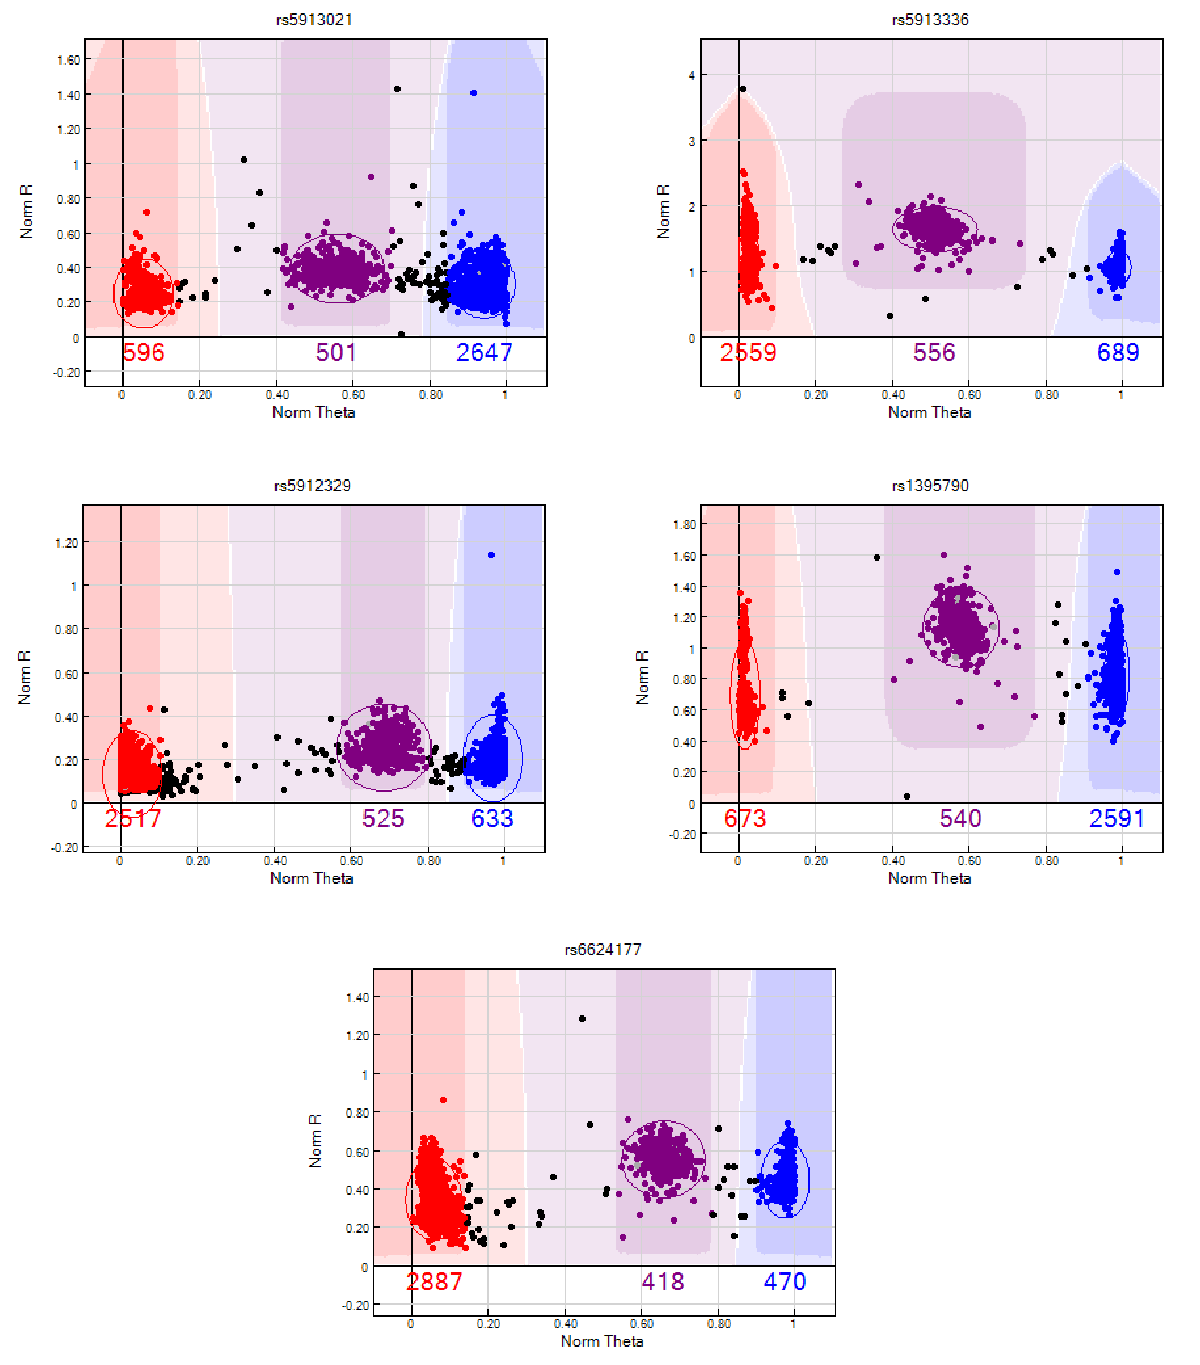
\includegraphics[width=\linewidth]{Figures/Table_One.pdf}
		\end{center}
		\caption{\textbf{Genotyping Cluster Plots of all SNPs in \ref{Table5}}}
		\label{Figure1C}

	\end{figure}

%%Cluster Plots - Table 2 
	\newpage
    \subsection{Cluster Plots of SNPs in Tier 2 Analysis}
	\begin{figure}[h!]
		\begin{center}
			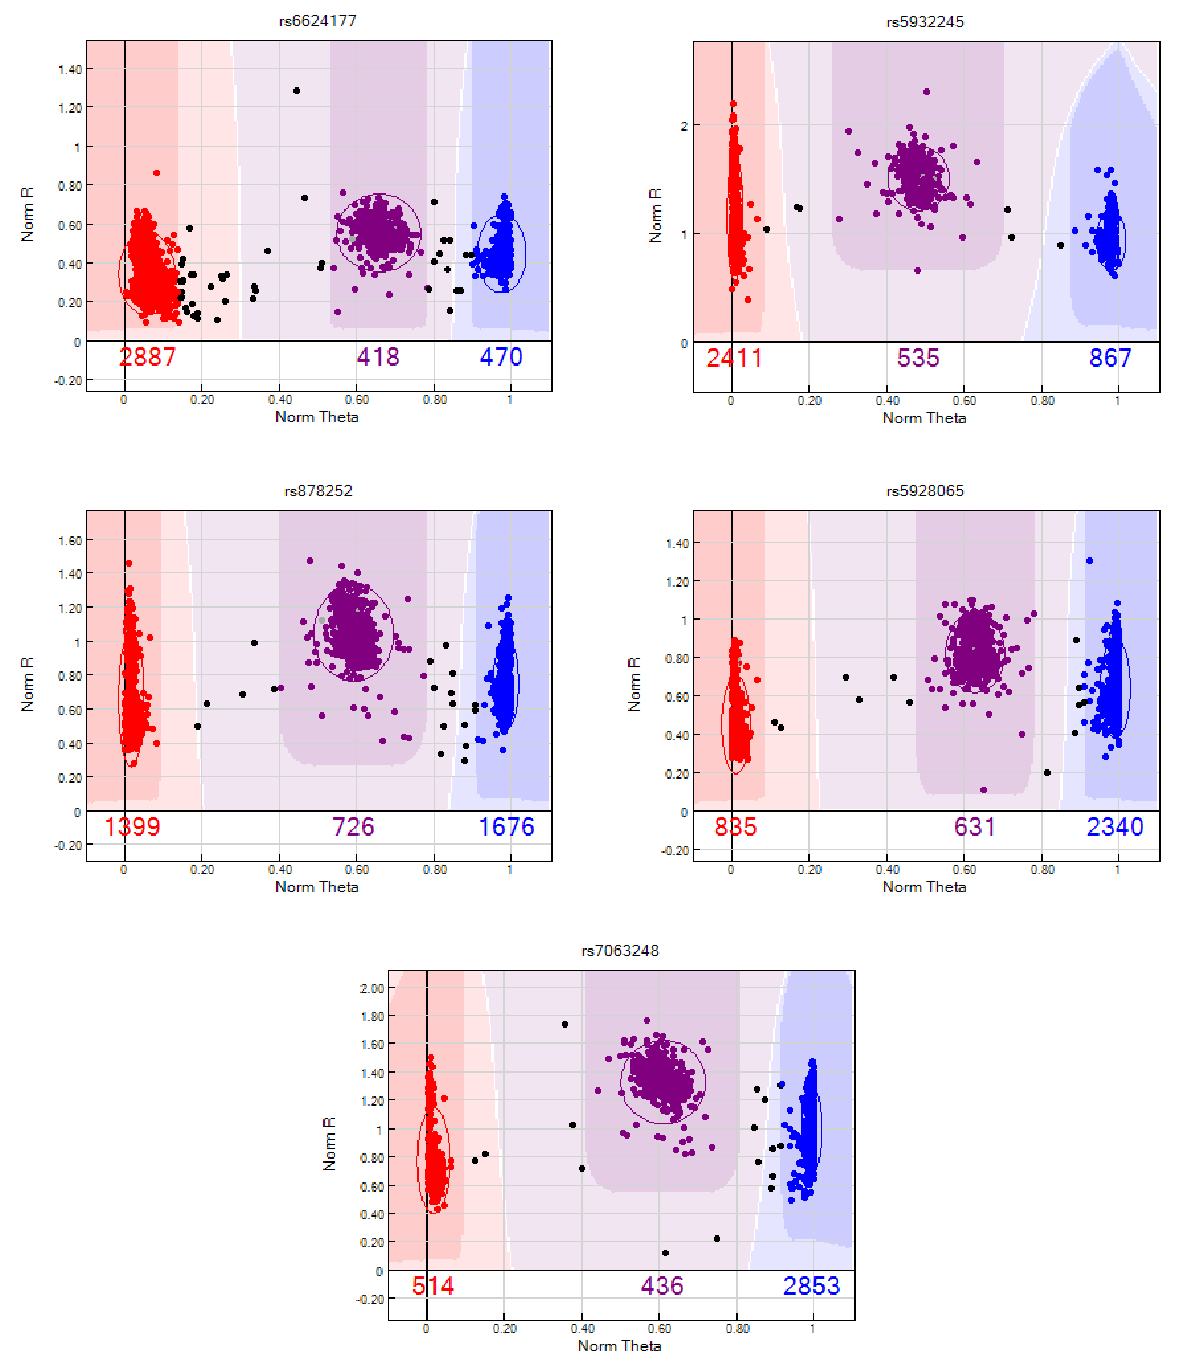
\includegraphics[width=\linewidth]{Figures/Table_two.pdf}
		\end{center}
		\caption{\textbf{Genotyping Cluster Plots of all SNPs in \ref{Table6}}}
	\label{Figure2C}
 
	\end{figure}

%%Cluster Plots - Table 3 
	\newpage
    \subsection{Cluster Plots of SNPs in Tier 3 Analysis}
	\begin{figure}[h!]
		\begin{center}
			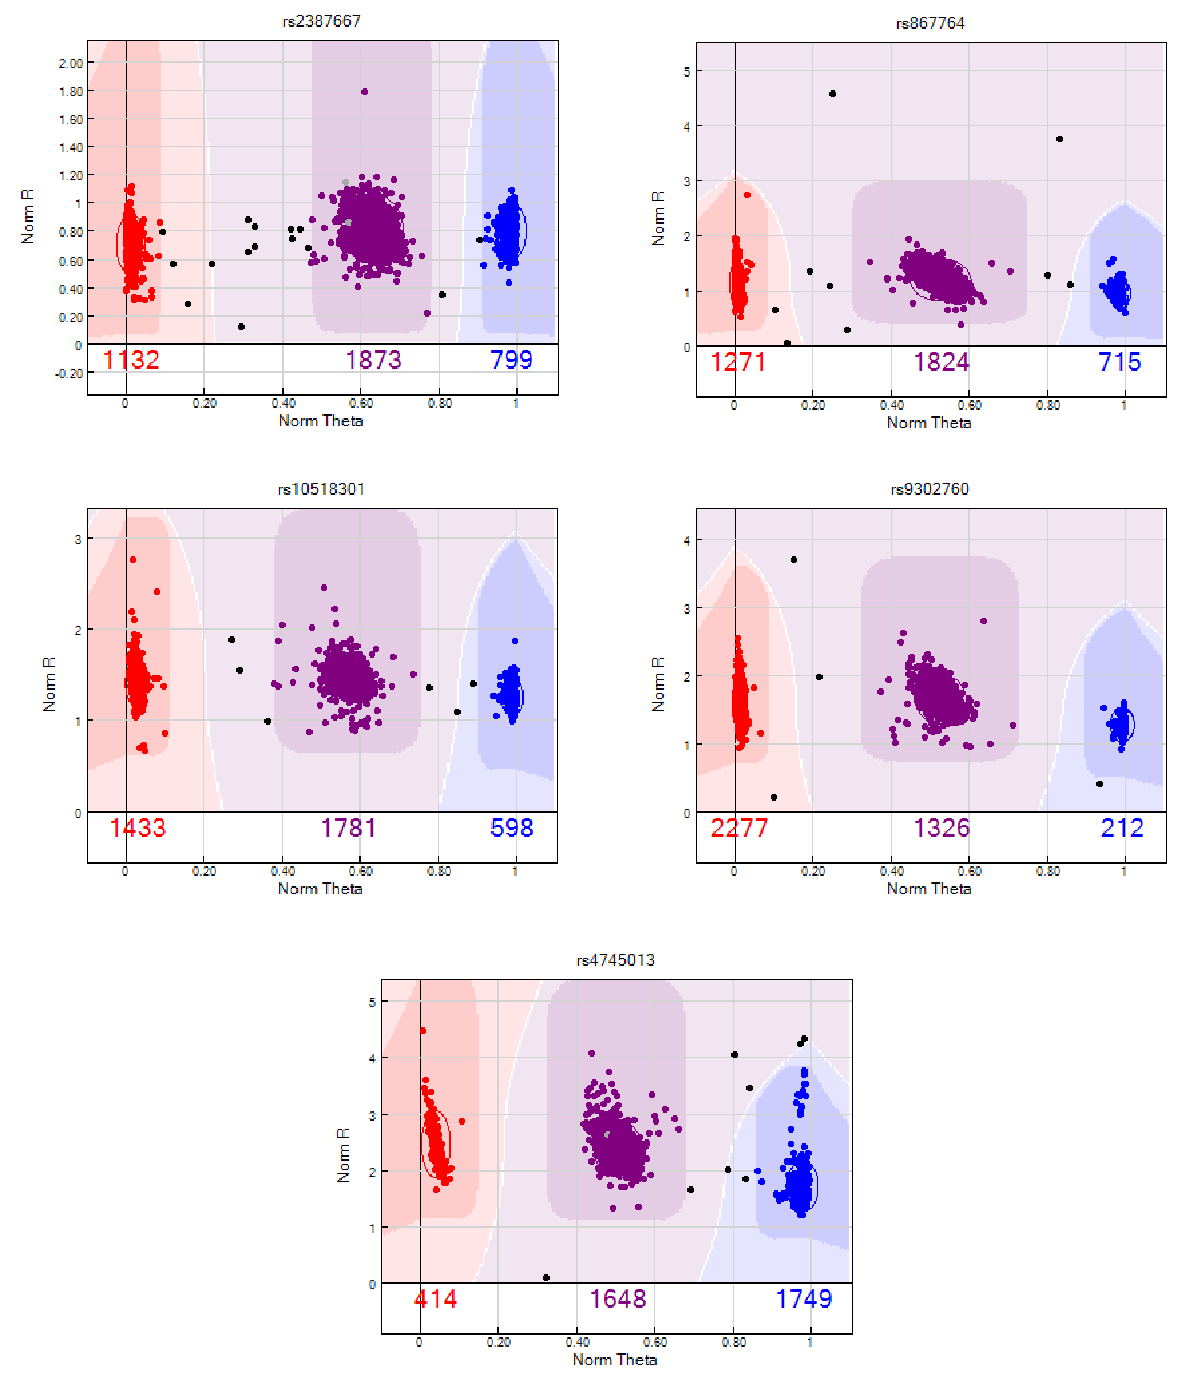
\includegraphics[width=\linewidth]{Figures/Table_three.pdf}
		\end{center}
		\caption{\textbf{Genotyping Cluster Plots of all SNPs in \ref{Table7}}}
		\label{Figure3C}

	\end{figure}


%%Cluster Plots - Supplement 1 of 6 
	\newpage
    	\subsection{Cluster Plots (1 through 5) of SNPs in Exploratory Analysis}
		\begin{figure}[h!]
		\begin{center}
			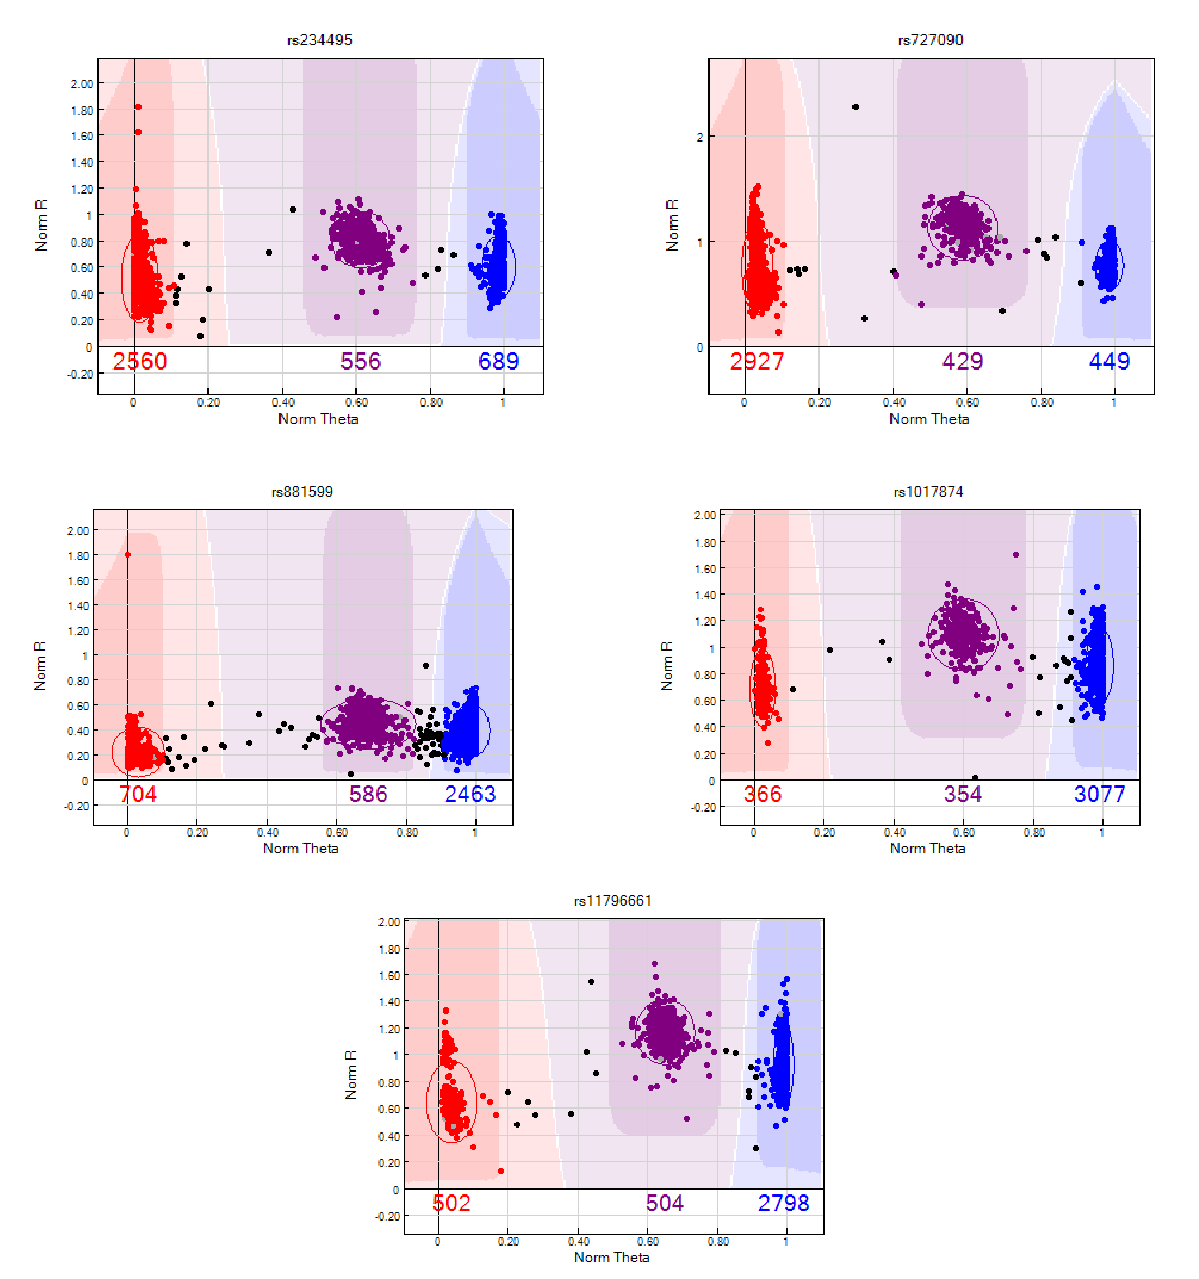
\includegraphics[width=\linewidth]{Figures/Panel_one.pdf}
		\end{center}
		\caption{\textbf{Genotyping Cluster Plots of SNPs in Exploratory Analysis Table \ref{Table4} \textit{(1 of 6)}}}
		\label{Figure4C1}

	\end{figure}

%%Cluster Plots - Supplement 2 of 6 
	\newpage
    \subsection{Cluster Plots (6 through 10) of SNPs in Exploratory Analysis}
		\begin{figure}[h!]
		\begin{center}
			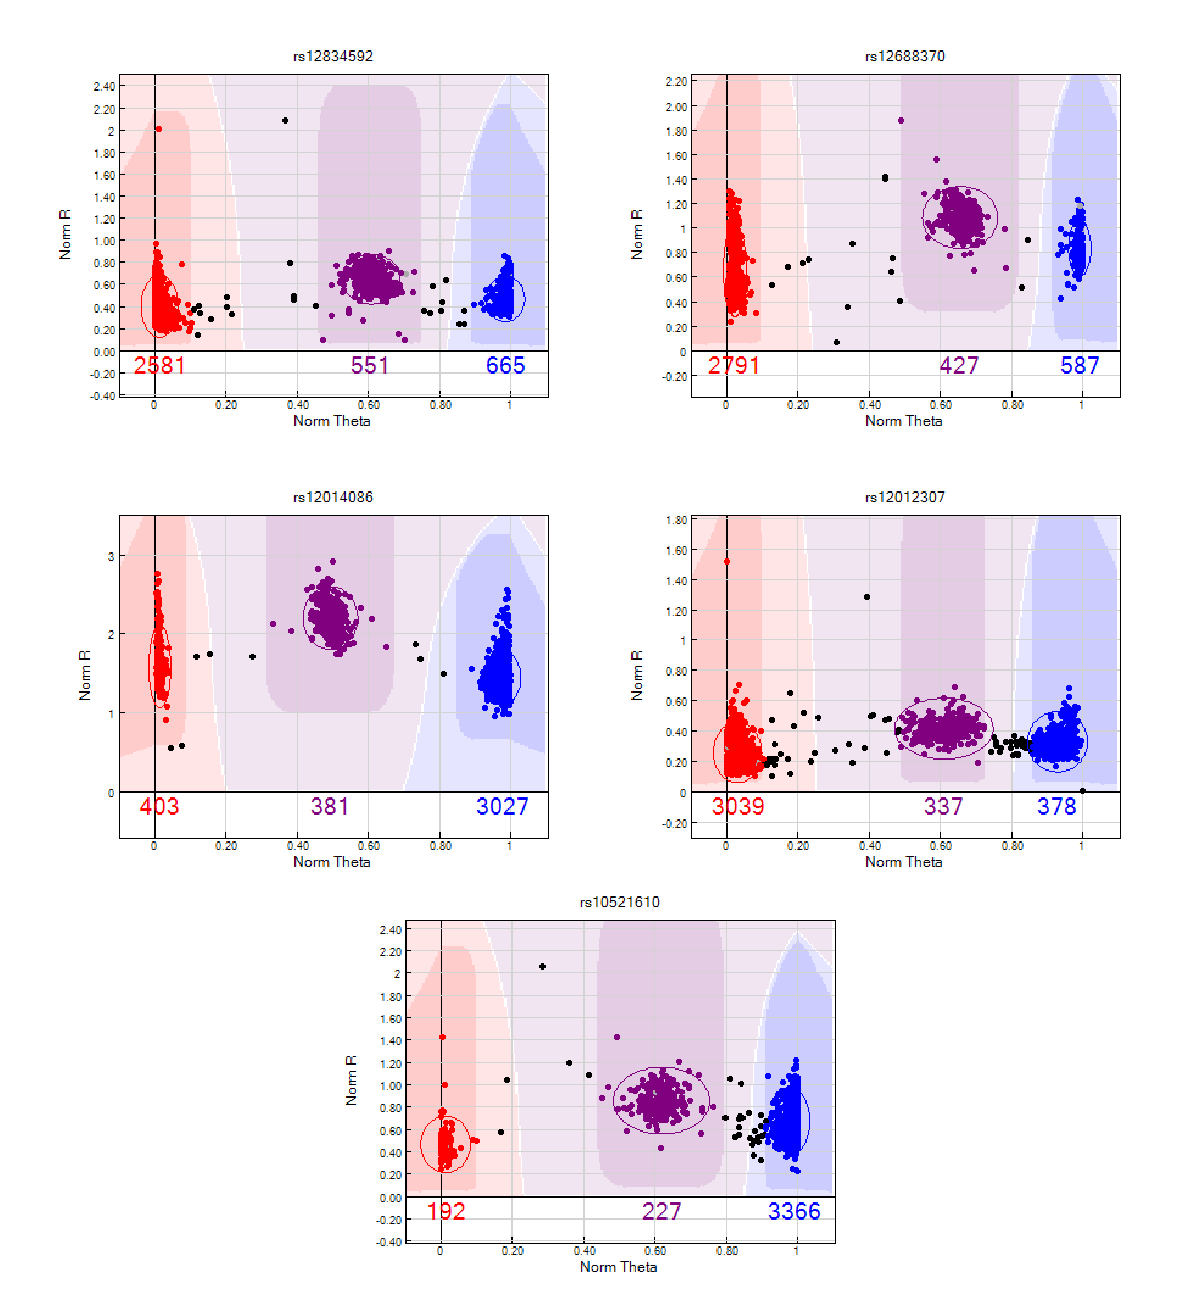
\includegraphics[width=\linewidth]{Figures/Panel_two.pdf}
		\end{center}
		\caption{\textbf{Genotyping Cluster Plots of SNPs in Exploratory Analysis Table \ref{Table4} \textit{(2 of 6)}}}
		\label{Figure4C2}

	\end{figure}

%%Cluster Plots - Supplement 3 of 6 
	\newpage
    	\subsection{Cluster Plots (11 through 15) of SNPs in Exploratory Analysis}
		\begin{figure}[h!]
		\begin{center}
			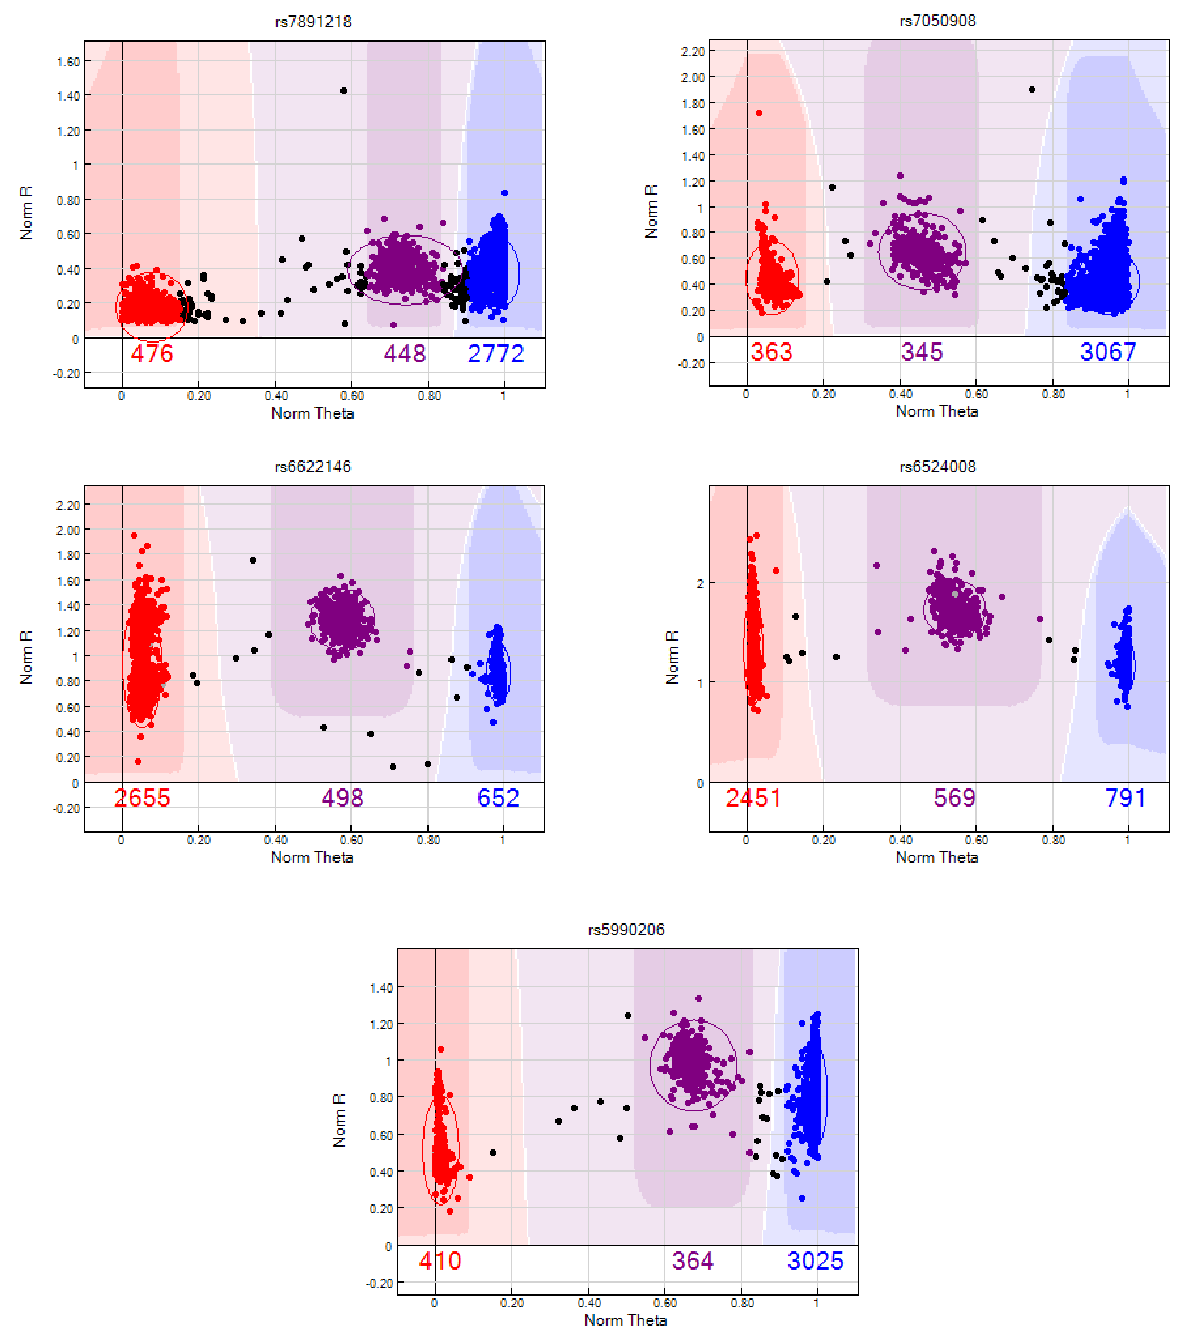
\includegraphics[width=\linewidth]{Figures/Panel_three.pdf}
		\end{center}
		\caption{\textbf{Genotyping Cluster Plots of SNPs in Exploratory Analysis Table \ref{Table4} \textit{(3 of 6)}}}
		\label{Figure4C3}

	\end{figure}

%%Cluster Plots - Supplement 4 of 6 
	\newpage
    \subsection{Cluster Plots (15 through 20) of SNPs in Exploratory Analysis}
	\begin{figure}[h!]
		\begin{center}
			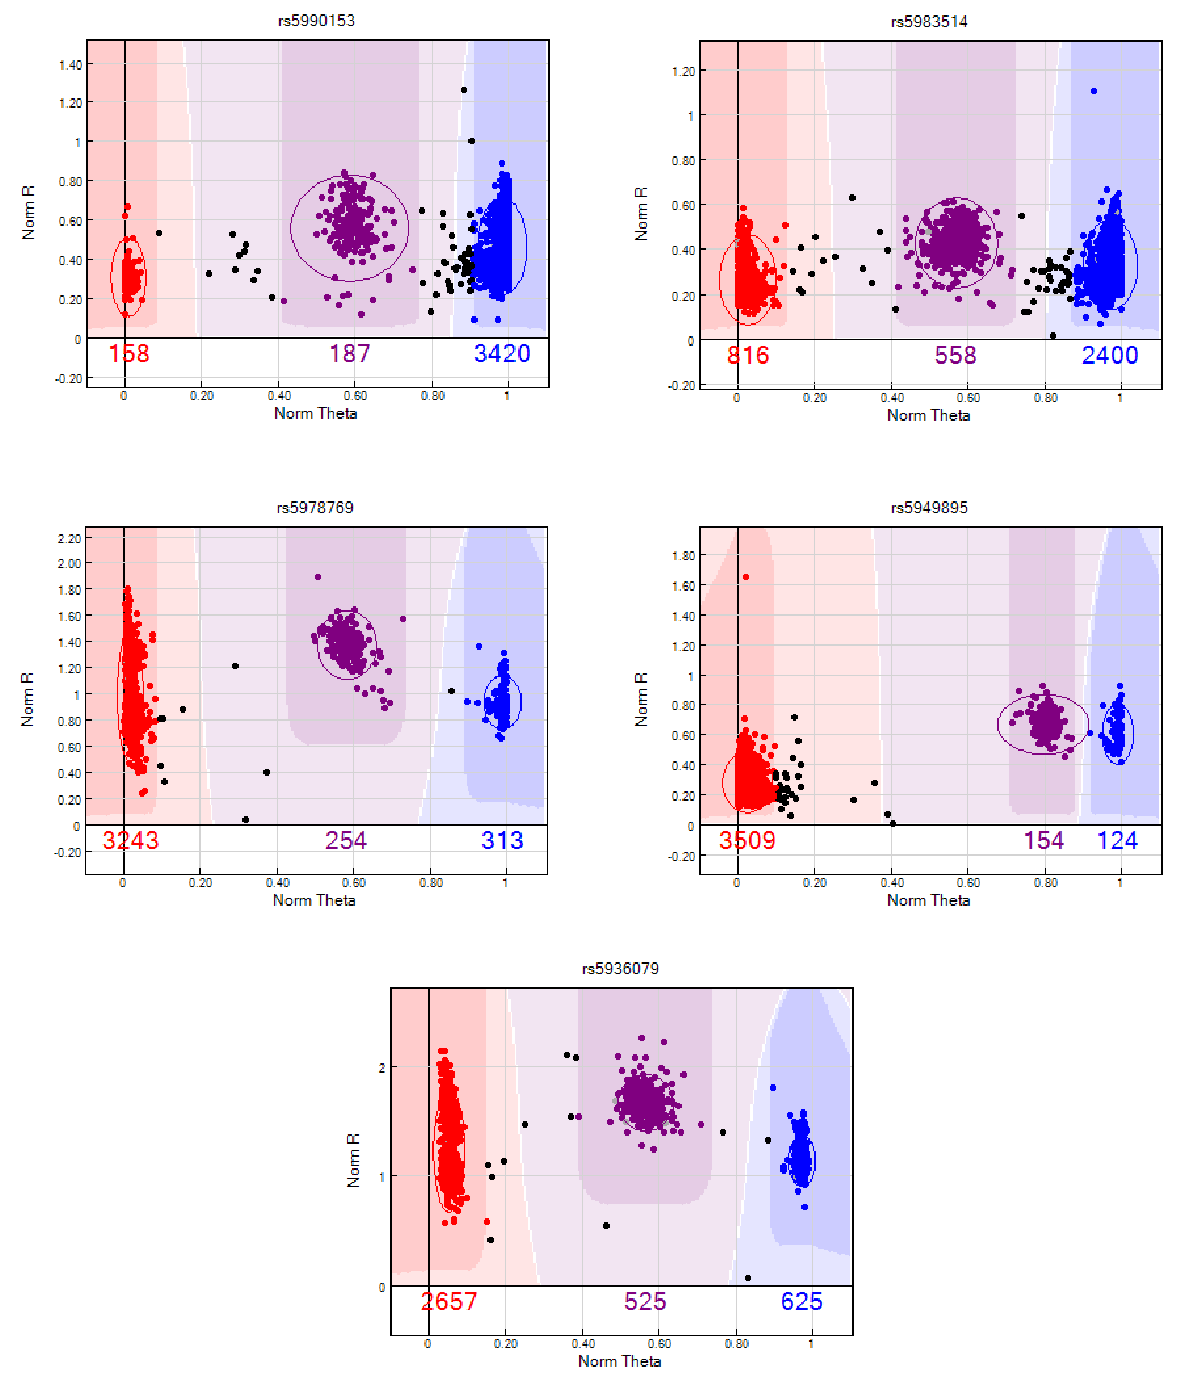
\includegraphics[width=\linewidth]{Figures/Panel_four.pdf}
		\end{center}
		\caption{\textbf{Genotyping Cluster Plots of SNPs in Exploratory Analysis Table \ref{Table4} \textit{(4 of 6)}}}
		\label{Figure4C4}

	\end{figure}

%%Cluster Plots - Supplement 5 of 6 
	\newpage
    \subsection{Cluster Plots (20 through 25) of SNPs in Exploratory Analysis}
	\begin{figure}[h!]
		\begin{center}
			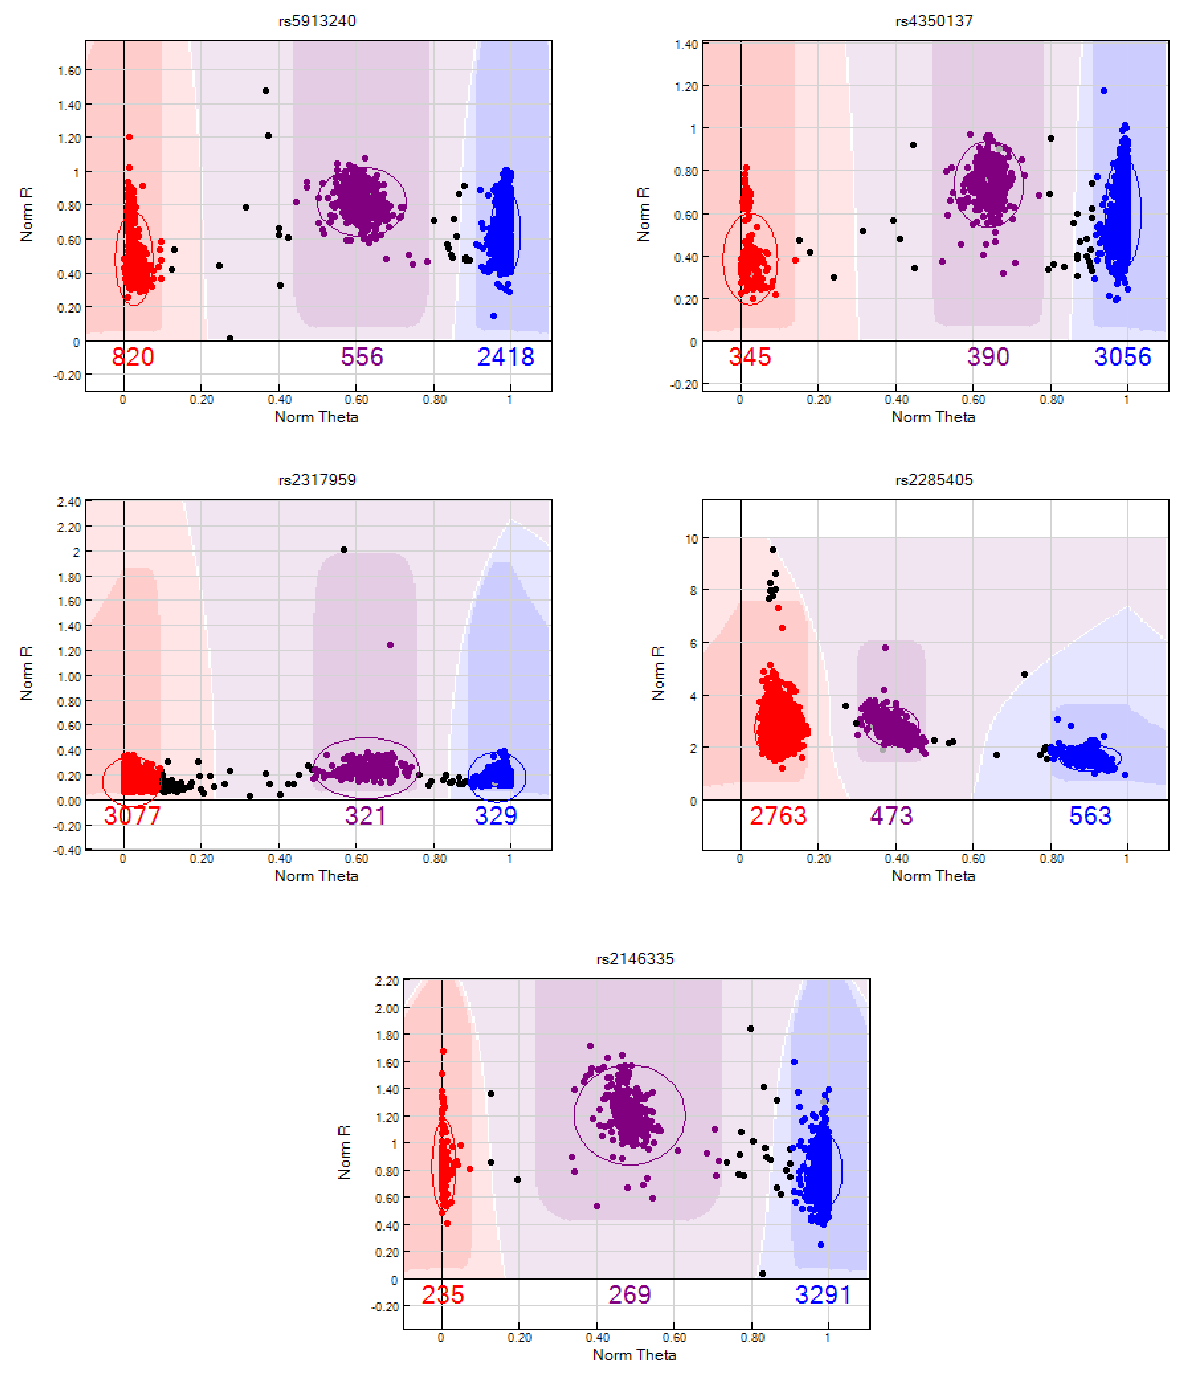
\includegraphics[width=\linewidth]{Figures/Panel_five.pdf}
		\end{center}
		\caption{\textbf{Genotyping Cluster Plots of SNPs in Exploratory Analysis Table \ref{Table4} \textit{(5 of 6)}}}
		\label{Figure4C5}

	\end{figure}

%%Cluster Plots - Supplement 6 of 6 
	\newpage
    \subsection{Cluster Plots (25 through 30) of SNPs in Exploratory Analysis}
	\begin{figure}[h!]
		\begin{center}
			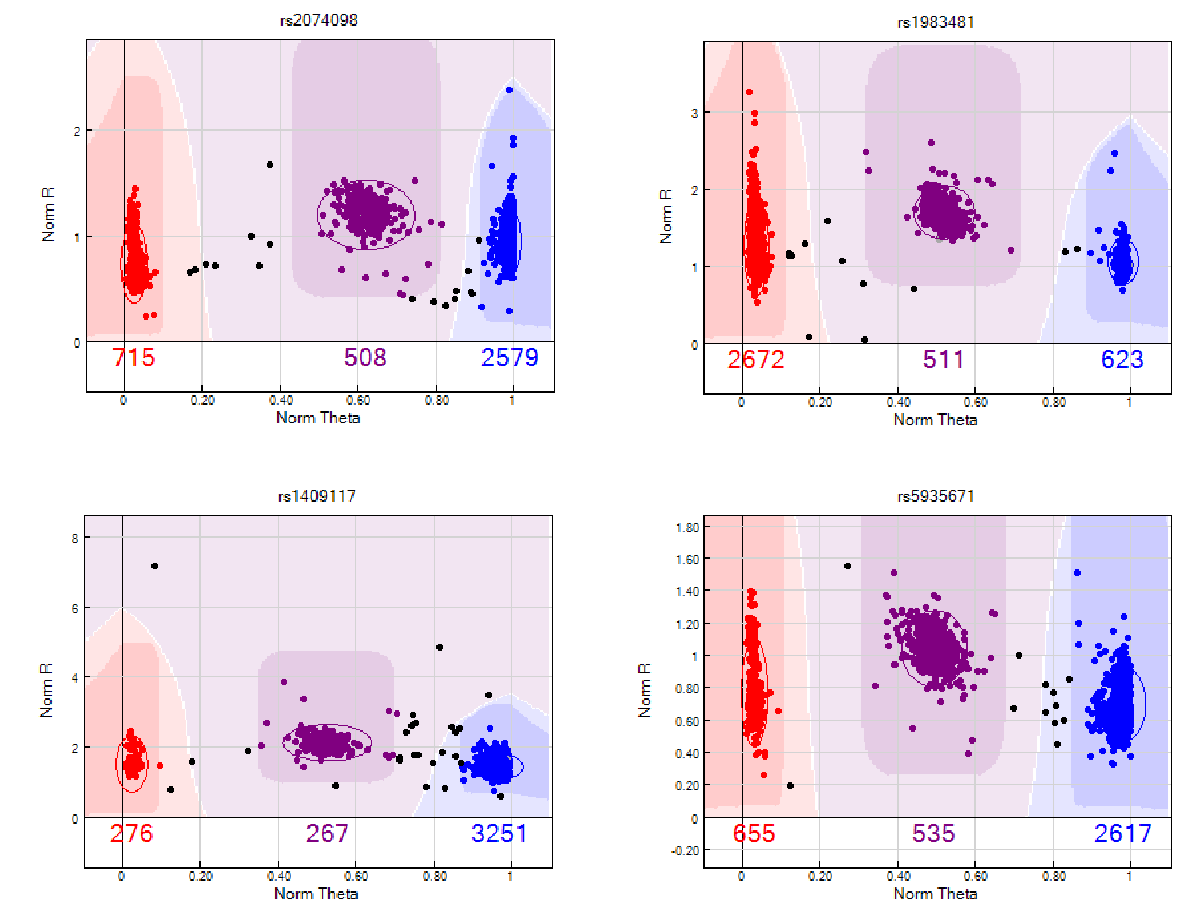
\includegraphics[width=\linewidth]{Figures/Panel_six.pdf}
		\end{center}
		\caption{\textbf{Genotyping Cluster Plots of SNPs in Exploratory Analysis Table \ref{Table4} \textit{(6 of 6)}}}
		\label{Figure4C6} 
	\end{figure}


% Any chapters such as End Notes go after this.
\backmatter

\bibliography{Thesis_ASD}
% for your own sake, use a bibtex file, so all of the numbering of references will be done
% automatically.

\end{document}
